\documentclass[twoside]{book}

% Packages required by doxygen
\usepackage{fixltx2e}
\usepackage{calc}
\usepackage{doxygen}
\usepackage[export]{adjustbox} % also loads graphicx
\usepackage{graphicx}
\usepackage[utf8]{inputenc}
\usepackage{makeidx}
\usepackage{multicol}
\usepackage{multirow}
\PassOptionsToPackage{warn}{textcomp}
\usepackage{textcomp}
\usepackage[nointegrals]{wasysym}
\usepackage[table]{xcolor}

% Font selection
\usepackage[T1]{fontenc}
\usepackage[scaled=.90]{helvet}
\usepackage{courier}
\usepackage{amssymb}
\usepackage{sectsty}
\renewcommand{\familydefault}{\sfdefault}
\allsectionsfont{%
  \fontseries{bc}\selectfont%
  \color{darkgray}%
}
\renewcommand{\DoxyLabelFont}{%
  \fontseries{bc}\selectfont%
  \color{darkgray}%
}
\newcommand{\+}{\discretionary{\mbox{\scriptsize$\hookleftarrow$}}{}{}}

% Page & text layout
\usepackage{geometry}
\geometry{%
  a4paper,%
  top=2.5cm,%
  bottom=2.5cm,%
  left=2.5cm,%
  right=2.5cm%
}
\tolerance=750
\hfuzz=15pt
\hbadness=750
\setlength{\emergencystretch}{15pt}
\setlength{\parindent}{0cm}
\setlength{\parskip}{3ex plus 2ex minus 2ex}
\makeatletter
\renewcommand{\paragraph}{%
  \@startsection{paragraph}{4}{0ex}{-1.0ex}{1.0ex}{%
    \normalfont\normalsize\bfseries\SS@parafont%
  }%
}
\renewcommand{\subparagraph}{%
  \@startsection{subparagraph}{5}{0ex}{-1.0ex}{1.0ex}{%
    \normalfont\normalsize\bfseries\SS@subparafont%
  }%
}
\makeatother

% Headers & footers
\usepackage{fancyhdr}
\pagestyle{fancyplain}
\fancyhead[LE]{\fancyplain{}{\bfseries\thepage}}
\fancyhead[CE]{\fancyplain{}{}}
\fancyhead[RE]{\fancyplain{}{\bfseries\leftmark}}
\fancyhead[LO]{\fancyplain{}{\bfseries\rightmark}}
\fancyhead[CO]{\fancyplain{}{}}
\fancyhead[RO]{\fancyplain{}{\bfseries\thepage}}
\fancyfoot[LE]{\fancyplain{}{}}
\fancyfoot[CE]{\fancyplain{}{}}
\fancyfoot[RE]{\fancyplain{}{\bfseries\scriptsize Generated by Doxygen }}
\fancyfoot[LO]{\fancyplain{}{\bfseries\scriptsize Generated by Doxygen }}
\fancyfoot[CO]{\fancyplain{}{}}
\fancyfoot[RO]{\fancyplain{}{}}
\renewcommand{\footrulewidth}{0.4pt}
\renewcommand{\chaptermark}[1]{%
  \markboth{#1}{}%
}
\renewcommand{\sectionmark}[1]{%
  \markright{\thesection\ #1}%
}

% Indices & bibliography
\usepackage{natbib}
\usepackage[titles]{tocloft}
\setcounter{tocdepth}{3}
\setcounter{secnumdepth}{5}
\makeindex

% Hyperlinks (required, but should be loaded last)
\usepackage{ifpdf}
\ifpdf
  \usepackage[pdftex,pagebackref=true]{hyperref}
\else
  \usepackage[ps2pdf,pagebackref=true]{hyperref}
\fi
\hypersetup{%
  colorlinks=true,%
  linkcolor=blue,%
  citecolor=blue,%
  unicode%
}

% Custom commands
\newcommand{\clearemptydoublepage}{%
  \newpage{\pagestyle{empty}\cleardoublepage}%
}

\usepackage{caption}
\captionsetup{labelsep=space,justification=centering,font={bf},singlelinecheck=off,skip=4pt,position=top}

%===== C O N T E N T S =====

\begin{document}

% Titlepage & ToC
\hypersetup{pageanchor=false,
             bookmarksnumbered=true,
             pdfencoding=unicode
            }
\pagenumbering{roman}
\begin{titlepage}
\vspace*{7cm}
\begin{center}%
{\Large bingocpp }\\
\vspace*{1cm}
{\large Generated by Doxygen 1.8.11}\\
\end{center}
\end{titlepage}
\clearemptydoublepage
\tableofcontents
\clearemptydoublepage
\pagenumbering{arabic}
\hypersetup{pageanchor=true}

%--- Begin generated contents ---
\chapter{Bingo\+Cpp}
\label{index}\hypertarget{index}{}master\+: \href{https://travis-ci.com/nasa/bingocpp}{\tt } \href{https://coveralls.io/github/nasa/bingocpp?branch=master}{\tt }

develop\+: \href{https://travis-ci.com/nasa/bingocpp}{\tt } \href{https://coveralls.io/github/nasa/bingocpp?branch=develop}{\tt } \href{https://www.codacy.com/app/bingo_developers/bingocpp?utm_source=github.com&amp;utm_medium=referral&amp;utm_content=nasa/bingocpp&amp;utm_campaign=Badge_Grade}{\tt }

\subsection*{General}

Bingocpp is part of the open source package Bingo for performing symbolic regression. Bingocpp contains the c++ implementation of a portion of the code within bingo.

\subsection*{Dependencies}

The build process requires\+:
\begin{DoxyItemize}
\item A recent version of cmake
\item git
\item mercurial (hg)
\end{DoxyItemize}

The other follwoing dependencies will automatically be downloaded and installed as part of the cmake build\+:
\begin{DoxyItemize}
\item google test (gtest), as part of the testing suite
\item pybind, for the python bindings
\item eigen, for much of the linear algebra and vectorized math
\end{DoxyItemize}

\subsection*{Tests}

Several unit and integration tests will be made upon building. You can run the testing suite by running the \char`\"{}run\+\_\+tests\char`\"{} executable in the build folder.

\subsection*{Notices}

Copyright 2018 United States Government as represented by the Administrator of the National Aeronautics and Space Administration. No copyright is claimed in the United States under Title 17, U.\+S. Code. All Other Rights Reserved.

\subsection*{Disclaimers}

No Warranty\+: T\+HE S\+U\+B\+J\+E\+CT S\+O\+F\+T\+W\+A\+RE IS P\+R\+O\+V\+I\+D\+ED \char`\"{}\+A\+S I\+S\char`\"{} W\+I\+T\+H\+O\+UT A\+NY W\+A\+R\+R\+A\+N\+TY OF A\+NY K\+I\+ND, E\+I\+T\+H\+ER E\+X\+P\+R\+E\+S\+S\+ED, I\+M\+P\+L\+I\+ED, OR S\+T\+A\+T\+U\+T\+O\+RY, I\+N\+C\+L\+U\+D\+I\+NG, B\+UT N\+OT L\+I\+M\+I\+T\+ED TO, A\+NY W\+A\+R\+R\+A\+N\+TY T\+H\+AT T\+HE S\+U\+B\+J\+E\+CT S\+O\+F\+T\+W\+A\+RE W\+I\+LL C\+O\+N\+F\+O\+RM TO S\+P\+E\+C\+I\+F\+I\+C\+A\+T\+I\+O\+NS, A\+NY I\+M\+P\+L\+I\+ED W\+A\+R\+R\+A\+N\+T\+I\+ES OF M\+E\+R\+C\+H\+A\+N\+T\+A\+B\+I\+L\+I\+TY, F\+I\+T\+N\+E\+SS F\+OR A P\+A\+R\+T\+I\+C\+U\+L\+AR P\+U\+R\+P\+O\+SE, OR F\+R\+E\+E\+D\+OM F\+R\+OM I\+N\+F\+R\+I\+N\+G\+E\+M\+E\+NT, A\+NY W\+A\+R\+R\+A\+N\+TY T\+H\+AT T\+HE S\+U\+B\+J\+E\+CT S\+O\+F\+T\+W\+A\+RE W\+I\+LL BE E\+R\+R\+OR F\+R\+EE, OR A\+NY W\+A\+R\+R\+A\+N\+TY T\+H\+AT D\+O\+C\+U\+M\+E\+N\+T\+A\+T\+I\+ON, IF P\+R\+O\+V\+I\+D\+ED, W\+I\+LL C\+O\+N\+F\+O\+RM TO T\+HE S\+U\+B\+J\+E\+CT S\+O\+F\+T\+W\+A\+RE. T\+H\+IS A\+G\+R\+E\+E\+M\+E\+NT D\+O\+ES N\+OT, IN A\+NY M\+A\+N\+N\+ER, C\+O\+N\+S\+T\+I\+T\+U\+TE AN E\+N\+D\+O\+R\+S\+E\+M\+E\+NT BY G\+O\+V\+E\+R\+N\+M\+E\+NT A\+G\+E\+N\+CY OR A\+NY P\+R\+I\+OR R\+E\+C\+I\+P\+I\+E\+NT OF A\+NY R\+E\+S\+U\+L\+TS, R\+E\+S\+U\+L\+T\+I\+NG D\+E\+S\+I\+G\+NS, H\+A\+R\+D\+W\+A\+RE, S\+O\+F\+T\+W\+A\+RE P\+R\+O\+D\+U\+C\+TS OR A\+NY O\+T\+H\+ER A\+P\+P\+L\+I\+C\+A\+T\+I\+O\+NS R\+E\+S\+U\+L\+T\+I\+NG F\+R\+OM U\+SE OF T\+HE S\+U\+B\+J\+E\+CT S\+O\+F\+T\+W\+A\+RE. F\+U\+R\+T\+H\+ER, G\+O\+V\+E\+R\+N\+M\+E\+NT A\+G\+E\+N\+CY D\+I\+S\+C\+L\+A\+I\+MS A\+LL W\+A\+R\+R\+A\+N\+T\+I\+ES A\+ND L\+I\+A\+B\+I\+L\+I\+T\+I\+ES R\+E\+G\+A\+R\+D\+I\+NG T\+H\+I\+R\+D-\/\+P\+A\+R\+TY S\+O\+F\+T\+W\+A\+RE, IF P\+R\+E\+S\+E\+NT IN T\+HE O\+R\+I\+G\+I\+N\+AL S\+O\+F\+T\+W\+A\+RE, A\+ND D\+I\+S\+T\+R\+I\+B\+U\+T\+ES IT \char`\"{}\+A\+S I\+S.\char`\"{}


Waiver and Indemnity\+: R\+E\+C\+I\+P\+I\+E\+NT A\+G\+R\+E\+ES TO W\+A\+I\+VE A\+NY A\+ND A\+LL C\+L\+A\+I\+MS A\+G\+A\+I\+N\+ST T\+HE U\+N\+I\+T\+ED S\+T\+A\+T\+ES G\+O\+V\+E\+R\+N\+M\+E\+NT, I\+TS C\+O\+N\+T\+R\+A\+C\+T\+O\+RS A\+ND S\+U\+B\+C\+O\+N\+T\+R\+A\+C\+T\+O\+RS, AS W\+E\+LL AS A\+NY P\+R\+I\+OR R\+E\+C\+I\+P\+I\+E\+NT. IF R\+E\+C\+I\+P\+I\+E\+NT\textquotesingle{}S U\+SE OF T\+HE S\+U\+B\+J\+E\+CT S\+O\+F\+T\+W\+A\+RE R\+E\+S\+U\+L\+TS IN A\+NY L\+I\+A\+B\+I\+L\+I\+T\+I\+ES, D\+E\+M\+A\+N\+DS, D\+A\+M\+A\+G\+ES, E\+X\+P\+E\+N\+S\+ES OR L\+O\+S\+S\+ES A\+R\+I\+S\+I\+NG F\+R\+OM S\+U\+CH U\+SE, I\+N\+C\+L\+U\+D\+I\+NG A\+NY D\+A\+M\+A\+G\+ES F\+R\+OM P\+R\+O\+D\+U\+C\+TS B\+A\+S\+ED ON, OR R\+E\+S\+U\+L\+T\+I\+NG F\+R\+OM, R\+E\+C\+I\+P\+I\+E\+NT\textquotesingle{}S U\+SE OF T\+HE S\+U\+B\+J\+E\+CT S\+O\+F\+T\+W\+A\+RE, R\+E\+C\+I\+P\+I\+E\+NT S\+H\+A\+LL I\+N\+D\+E\+M\+N\+I\+FY A\+ND H\+O\+LD H\+A\+R\+M\+L\+E\+SS T\+HE U\+N\+I\+T\+ED S\+T\+A\+T\+ES G\+O\+V\+E\+R\+N\+M\+E\+NT, I\+TS C\+O\+N\+T\+R\+A\+C\+T\+O\+RS A\+ND S\+U\+B\+C\+O\+N\+T\+R\+A\+C\+T\+O\+RS, AS W\+E\+LL AS A\+NY P\+R\+I\+OR R\+E\+C\+I\+P\+I\+E\+NT, TO T\+HE E\+X\+T\+E\+NT P\+E\+R\+M\+I\+T\+T\+ED BY L\+AW. R\+E\+C\+I\+P\+I\+E\+NT\textquotesingle{}S S\+O\+LE R\+E\+M\+E\+DY F\+OR A\+NY S\+U\+CH M\+A\+T\+T\+ER S\+H\+A\+LL BE T\+HE I\+M\+M\+E\+D\+I\+A\+TE, U\+N\+I\+L\+A\+T\+E\+R\+AL T\+E\+R\+M\+I\+N\+A\+T\+I\+ON OF T\+H\+IS A\+G\+R\+E\+E\+M\+E\+NT. 
\chapter{Hierarchical Index}
\section{Class Hierarchy}
This inheritance list is sorted roughly, but not completely, alphabetically\+:\begin{DoxyCompactList}
\item \contentsline{section}{Acyclic\+Graph}{\pageref{classAcyclicGraph}}{}
\item \contentsline{section}{Acyclic\+Graph\+Manipulator}{\pageref{classAcyclicGraphManipulator}}{}
\item \contentsline{section}{Fitness\+Metric}{\pageref{structFitnessMetric}}{}
\begin{DoxyCompactList}
\item \contentsline{section}{Implicit\+Regression}{\pageref{structImplicitRegression}}{}
\item \contentsline{section}{Standard\+Regression}{\pageref{structStandardRegression}}{}
\end{DoxyCompactList}
\item \contentsline{section}{L\+M\+Functor}{\pageref{structLMFunctor}}{}
\item \contentsline{section}{Operation}{\pageref{classOperation}}{}
\begin{DoxyCompactList}
\item \contentsline{section}{Absolute}{\pageref{classAbsolute}}{}
\item \contentsline{section}{Addition}{\pageref{classAddition}}{}
\item \contentsline{section}{C\+\_\+\+Load}{\pageref{classC__Load}}{}
\item \contentsline{section}{Cos}{\pageref{classCos}}{}
\item \contentsline{section}{Division}{\pageref{classDivision}}{}
\item \contentsline{section}{Exp}{\pageref{classExp}}{}
\item \contentsline{section}{Log}{\pageref{classLog}}{}
\item \contentsline{section}{Multiplication}{\pageref{classMultiplication}}{}
\item \contentsline{section}{Power}{\pageref{classPower}}{}
\item \contentsline{section}{Sin}{\pageref{classSin}}{}
\item \contentsline{section}{Sqrt}{\pageref{classSqrt}}{}
\item \contentsline{section}{Subtraction}{\pageref{classSubtraction}}{}
\item \contentsline{section}{X\+\_\+\+Load}{\pageref{classX__Load}}{}
\end{DoxyCompactList}
\item \contentsline{section}{Operator\+Interface}{\pageref{classOperatorInterface}}{}
\item \contentsline{section}{Training\+Data}{\pageref{structTrainingData}}{}
\begin{DoxyCompactList}
\item \contentsline{section}{Explicit\+Training\+Data}{\pageref{structExplicitTrainingData}}{}
\item \contentsline{section}{Implicit\+Training\+Data}{\pageref{structImplicitTrainingData}}{}
\end{DoxyCompactList}
\end{DoxyCompactList}

\chapter{Class Index}
\section{Class List}
Here are the classes, structs, unions and interfaces with brief descriptions\+:\begin{DoxyCompactList}
\item\contentsline{section}{\hyperlink{classAbsolute}{Absolute} \\*This class performs an absolute }{\pageref{classAbsolute}}{}
\item\contentsline{section}{\hyperlink{classAcyclicGraph}{Acyclic\+Graph} }{\pageref{classAcyclicGraph}}{}
\item\contentsline{section}{\hyperlink{classAcyclicGraphManipulator}{Acyclic\+Graph\+Manipulator} }{\pageref{classAcyclicGraphManipulator}}{}
\item\contentsline{section}{\hyperlink{classAddition}{Addition} \\*This class performs addition }{\pageref{classAddition}}{}
\item\contentsline{section}{\hyperlink{classC__Load}{C\+\_\+\+Load} \\*This class loads the constant }{\pageref{classC__Load}}{}
\item\contentsline{section}{\hyperlink{classCos}{Cos} \\*This class performs cosine }{\pageref{classCos}}{}
\item\contentsline{section}{\hyperlink{classDivision}{Division} \\*This class performs division }{\pageref{classDivision}}{}
\item\contentsline{section}{\hyperlink{classExp}{Exp} \\*This class performs an exponential }{\pageref{classExp}}{}
\item\contentsline{section}{\hyperlink{structExplicitTrainingData}{Explicit\+Training\+Data} \\*This struct holds data for Explicit regression }{\pageref{structExplicitTrainingData}}{}
\item\contentsline{section}{\hyperlink{structFitnessMetric}{Fitness\+Metric} }{\pageref{structFitnessMetric}}{}
\item\contentsline{section}{\hyperlink{structImplicitRegression}{Implicit\+Regression} \\*Implicit Regression }{\pageref{structImplicitRegression}}{}
\item\contentsline{section}{\hyperlink{structImplicitTrainingData}{Implicit\+Training\+Data} \\*This struct holds data for Implicit regression }{\pageref{structImplicitTrainingData}}{}
\item\contentsline{section}{\hyperlink{structLMFunctor}{L\+M\+Functor} }{\pageref{structLMFunctor}}{}
\item\contentsline{section}{\hyperlink{classLog}{Log} \\*This class performs a safe log }{\pageref{classLog}}{}
\item\contentsline{section}{\hyperlink{classMultiplication}{Multiplication} \\*This class performs multiplication }{\pageref{classMultiplication}}{}
\item\contentsline{section}{\hyperlink{classOperation}{Operation} \\*Abstract class for an operation }{\pageref{classOperation}}{}
\item\contentsline{section}{\hyperlink{classOperatorInterface}{Operator\+Interface} \\*Populate and hold the map of operations }{\pageref{classOperatorInterface}}{}
\item\contentsline{section}{\hyperlink{classPower}{Power} \\*This class performs power }{\pageref{classPower}}{}
\item\contentsline{section}{\hyperlink{classSin}{Sin} \\*This class performs sine }{\pageref{classSin}}{}
\item\contentsline{section}{\hyperlink{classSqrt}{Sqrt} \\*This class performs square root }{\pageref{classSqrt}}{}
\item\contentsline{section}{\hyperlink{structStandardRegression}{Standard\+Regression} \\*Traditional fitness evaluation }{\pageref{structStandardRegression}}{}
\item\contentsline{section}{\hyperlink{classSubtraction}{Subtraction} \\*This class performs subtraction }{\pageref{classSubtraction}}{}
\item\contentsline{section}{\hyperlink{structTrainingData}{Training\+Data} }{\pageref{structTrainingData}}{}
\item\contentsline{section}{\hyperlink{classX__Load}{X\+\_\+\+Load} \\*This class loads the X }{\pageref{classX__Load}}{}
\end{DoxyCompactList}

\chapter{File Index}
\section{File List}
Here is a list of all documented files with brief descriptions\+:\begin{DoxyCompactList}
\item\contentsline{section}{/users0/gbomarit/\+Projects/\+Genetic\+\_\+\+Programming/bingo/bingocpp/include/\+Bingo\+Cpp/{\bfseries acyclic\+\_\+graph.\+h} }{\pageref{acyclic__graph_8h}}{}
\item\contentsline{section}{/users0/gbomarit/\+Projects/\+Genetic\+\_\+\+Programming/bingo/bingocpp/include/\+Bingo\+Cpp/{\bfseries acyclic\+\_\+graph\+\_\+nodes.\+h} }{\pageref{acyclic__graph__nodes_8h}}{}
\item\contentsline{section}{/users0/gbomarit/\+Projects/\+Genetic\+\_\+\+Programming/bingo/bingocpp/include/\+Bingo\+Cpp/\hyperlink{fitness__metric_8h}{fitness\+\_\+metric.\+h} }{\pageref{fitness__metric_8h}}{}
\item\contentsline{section}{/users0/gbomarit/\+Projects/\+Genetic\+\_\+\+Programming/bingo/bingocpp/include/\+Bingo\+Cpp/\hyperlink{graph__manip_8h}{graph\+\_\+manip.\+h} }{\pageref{graph__manip_8h}}{}
\item\contentsline{section}{/users0/gbomarit/\+Projects/\+Genetic\+\_\+\+Programming/bingo/bingocpp/include/\+Bingo\+Cpp/\hyperlink{training__data_8h}{training\+\_\+data.\+h} }{\pageref{training__data_8h}}{}
\item\contentsline{section}{/users0/gbomarit/\+Projects/\+Genetic\+\_\+\+Programming/bingo/bingocpp/include/\+Bingo\+Cpp/\hyperlink{utils_8h}{utils.\+h} }{\pageref{utils_8h}}{}
\item\contentsline{section}{/users0/gbomarit/\+Projects/\+Genetic\+\_\+\+Programming/bingo/bingocpp/include/\+Bingo\+Cpp/{\bfseries version.\+h} }{\pageref{version_8h}}{}
\end{DoxyCompactList}

\chapter{Class Documentation}
\hypertarget{classAbsolute}{}\section{Absolute Class Reference}
\label{classAbsolute}\index{Absolute@{Absolute}}


This class performs an absolute.  




{\ttfamily \#include $<$acyclic\+\_\+graph\+\_\+nodes.\+h$>$}

Inheritance diagram for Absolute\+:\begin{figure}[H]
\begin{center}
\leavevmode
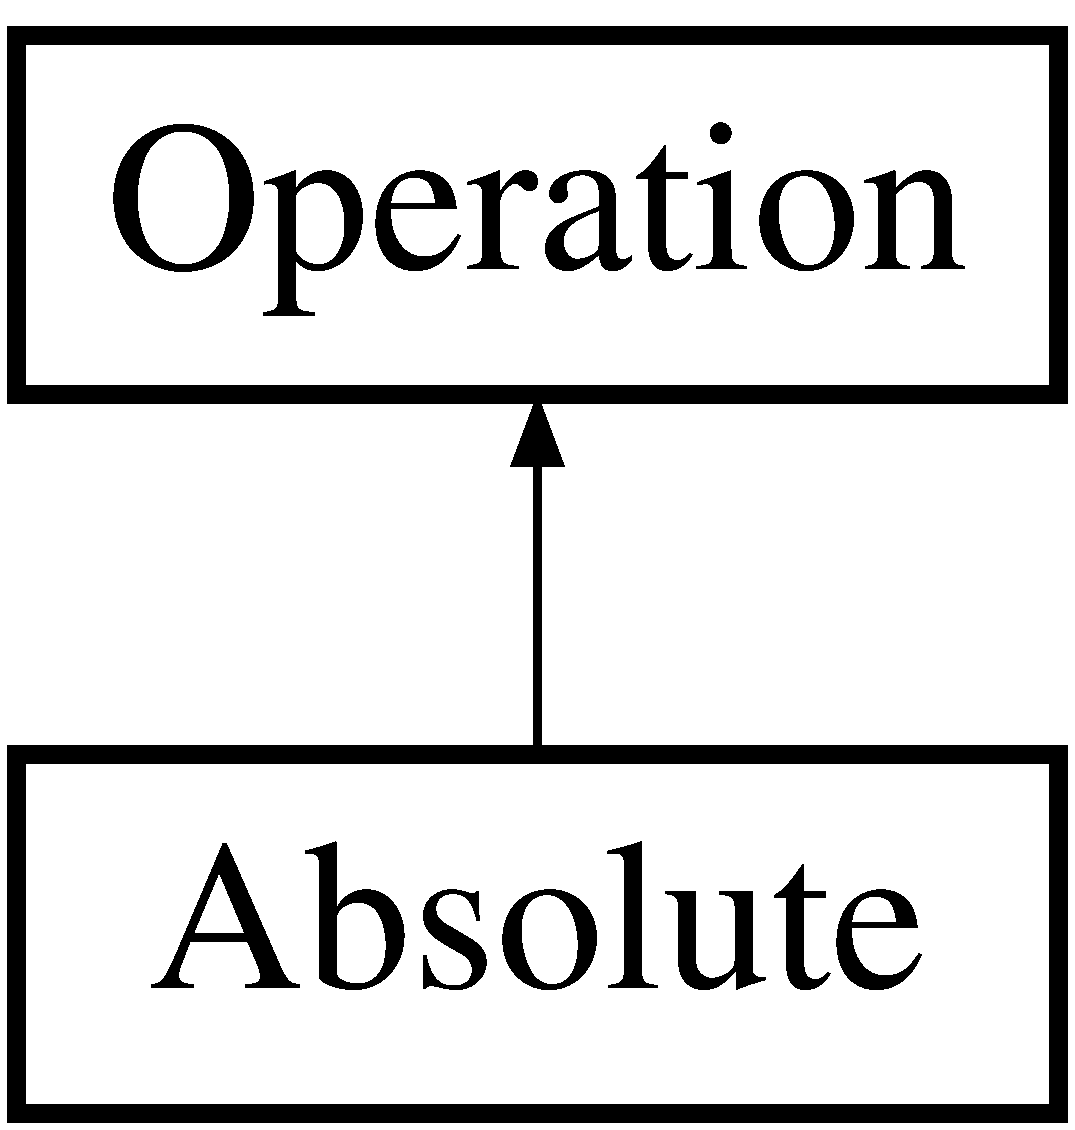
\includegraphics[height=2.000000cm]{classAbsolute}
\end{center}
\end{figure}
\subsection*{Public Member Functions}
\begin{DoxyCompactItemize}
\item 
int \hyperlink{classAbsolute_afb371f8c2c449e1d3b6d7f7a87621873}{get\+\_\+arity} ()\hypertarget{classAbsolute_afb371f8c2c449e1d3b6d7f7a87621873}{}\label{classAbsolute_afb371f8c2c449e1d3b6d7f7a87621873}

\begin{DoxyCompactList}\small\item\em Returns how many parameters the operation requires. \end{DoxyCompactList}\item 
std\+::string \hyperlink{classAbsolute_a18f5a749b8691c91d30c274603b3917e}{get\+\_\+print} ()\hypertarget{classAbsolute_a18f5a749b8691c91d30c274603b3917e}{}\label{classAbsolute_a18f5a749b8691c91d30c274603b3917e}

\begin{DoxyCompactList}\small\item\em Returns the string representation of the operator. \end{DoxyCompactList}\item 
virtual void \hyperlink{classAbsolute_a841ddbf6d5c0e8ad3950208946f9ad75}{evaluate} (const Eigen\+::\+Array\+X3i \&stack, const Eigen\+::\+Array\+X\+Xd \&x, const Eigen\+::\+Vector\+Xd \&constants, std\+::vector$<$ Eigen\+::\+Array\+X\+Xd $>$ \&buffer, std\+::size\+\_\+t result\+\_\+location)
\begin{DoxyCompactList}\small\item\em evaluates a single command at the location passed in \end{DoxyCompactList}\item 
virtual void \hyperlink{classAbsolute_a8c75e9e1efcfd1fc50ee2af13ed9d6d1}{deriv\+\_\+evaluate} (const Eigen\+::\+Array\+X3i \&stack, const int command\+\_\+index, const std\+::vector$<$ Eigen\+::\+Array\+X\+Xd $>$ \&forward\+\_\+buffer, std\+::vector$<$ Eigen\+::\+Array\+X\+Xd $>$ \&reverse\+\_\+buffer, int dependency)
\begin{DoxyCompactList}\small\item\em Computes reverse autodiff partial of a command stack. \end{DoxyCompactList}\end{DoxyCompactItemize}


\subsection{Detailed Description}
This class performs an absolute. 

\subsection{Member Function Documentation}
\index{Absolute@{Absolute}!deriv\+\_\+evaluate@{deriv\+\_\+evaluate}}
\index{deriv\+\_\+evaluate@{deriv\+\_\+evaluate}!Absolute@{Absolute}}
\subsubsection[{\texorpdfstring{deriv\+\_\+evaluate(const Eigen\+::\+Array\+X3i \&stack, const int command\+\_\+index, const std\+::vector$<$ Eigen\+::\+Array\+X\+Xd $>$ \&forward\+\_\+buffer, std\+::vector$<$ Eigen\+::\+Array\+X\+Xd $>$ \&reverse\+\_\+buffer, int dependency)}{deriv_evaluate(const Eigen::ArrayX3i &stack, const int command_index, const std::vector< Eigen::ArrayXXd > &forward_buffer, std::vector< Eigen::ArrayXXd > &reverse_buffer, int dependency)}}]{\setlength{\rightskip}{0pt plus 5cm}void Absolute\+::deriv\+\_\+evaluate (
\begin{DoxyParamCaption}
\item[{const Eigen\+::\+Array\+X3i \&}]{stack, }
\item[{const int}]{command\+\_\+index, }
\item[{const std\+::vector$<$ Eigen\+::\+Array\+X\+Xd $>$ \&}]{forward\+\_\+buffer, }
\item[{std\+::vector$<$ Eigen\+::\+Array\+X\+Xd $>$ \&}]{reverse\+\_\+buffer, }
\item[{int}]{dependency}
\end{DoxyParamCaption}
)\hspace{0.3cm}{\ttfamily [virtual]}}\hypertarget{classAbsolute_a8c75e9e1efcfd1fc50ee2af13ed9d6d1}{}\label{classAbsolute_a8c75e9e1efcfd1fc50ee2af13ed9d6d1}


Computes reverse autodiff partial of a command stack. 


\begin{DoxyParams}[1]{Parameters}
\mbox{\tt in}  & {\em stack} & The stack that contains each command. Eigen\+::\+Array\+X3i \\
\hline
\mbox{\tt in}  & {\em command\+\_\+index} & Index of command in the command; also the location of the result to be placed in the reverse buffer. \\
\hline
\mbox{\tt in}  & {\em forward\+\_\+buffer} & Vector of Eigen arrays for the forward buffer. \\
\hline
 & {\em } & \\
\hline
\end{DoxyParams}


Implements \hyperlink{classOperation_a42b611d08c6b00568c5d1b08688ebcce}{Operation}.

\index{Absolute@{Absolute}!evaluate@{evaluate}}
\index{evaluate@{evaluate}!Absolute@{Absolute}}
\subsubsection[{\texorpdfstring{evaluate(const Eigen\+::\+Array\+X3i \&stack, const Eigen\+::\+Array\+X\+Xd \&x, const Eigen\+::\+Vector\+Xd \&constants, std\+::vector$<$ Eigen\+::\+Array\+X\+Xd $>$ \&buffer, std\+::size\+\_\+t result\+\_\+location)}{evaluate(const Eigen::ArrayX3i &stack, const Eigen::ArrayXXd &x, const Eigen::VectorXd &constants, std::vector< Eigen::ArrayXXd > &buffer, std::size_t result_location)}}]{\setlength{\rightskip}{0pt plus 5cm}void Absolute\+::evaluate (
\begin{DoxyParamCaption}
\item[{const Eigen\+::\+Array\+X3i \&}]{stack, }
\item[{const Eigen\+::\+Array\+X\+Xd \&}]{x, }
\item[{const Eigen\+::\+Vector\+Xd \&}]{constants, }
\item[{std\+::vector$<$ Eigen\+::\+Array\+X\+Xd $>$ \&}]{buffer, }
\item[{std\+::size\+\_\+t}]{result\+\_\+location}
\end{DoxyParamCaption}
)\hspace{0.3cm}{\ttfamily [virtual]}}\hypertarget{classAbsolute_a841ddbf6d5c0e8ad3950208946f9ad75}{}\label{classAbsolute_a841ddbf6d5c0e8ad3950208946f9ad75}


evaluates a single command at the location passed in 


\begin{DoxyParams}[1]{Parameters}
\mbox{\tt in}  & {\em stack} & The stack that contains each command. Eigen\+::\+Array\+X3i \\
\hline
\mbox{\tt in}  & {\em x} & Input variables to the acyclic graph. Eigen\+::\+Array\+X\+Xd \\
\hline
\mbox{\tt in}  & {\em constants} & Constants used in the command. Eigen\+::\+Vector\+Xd \\
\hline
 & {\em } & \\
\hline
\end{DoxyParams}


Implements \hyperlink{classOperation_a89093eb53f975dd98b6a36d85fa17276}{Operation}.



The documentation for this class was generated from the following files\+:\begin{DoxyCompactItemize}
\item 
/users0/gbomarit/\+Projects/\+Genetic\+\_\+\+Programming/bingo/bingocpp/include/\+Bingo\+Cpp/acyclic\+\_\+graph\+\_\+nodes.\+h\item 
/users0/gbomarit/\+Projects/\+Genetic\+\_\+\+Programming/bingo/bingocpp/src/acyclic\+\_\+graph\+\_\+nodes.\+cpp\end{DoxyCompactItemize}

\hypertarget{classAcyclicGraph}{}\section{Acyclic\+Graph Class Reference}
\label{classAcyclicGraph}\index{Acyclic\+Graph@{Acyclic\+Graph}}


{\ttfamily \#include $<$graph\+\_\+manip.\+h$>$}

\subsection*{Public Member Functions}
\begin{DoxyCompactItemize}
\item 
\hyperlink{classAcyclicGraph_a939b4fffe09d7157d334509bdf8ce2be}{Acyclic\+Graph} ()\hypertarget{classAcyclicGraph_a939b4fffe09d7157d334509bdf8ce2be}{}\label{classAcyclicGraph_a939b4fffe09d7157d334509bdf8ce2be}

\begin{DoxyCompactList}\small\item\em Default constructor. \end{DoxyCompactList}\item 
\hyperlink{classAcyclicGraph_ab76060134cbc2754f3200f57da385ad2}{Acyclic\+Graph} (const \hyperlink{classAcyclicGraph}{Acyclic\+Graph} \&ag)\hypertarget{classAcyclicGraph_ab76060134cbc2754f3200f57da385ad2}{}\label{classAcyclicGraph_ab76060134cbc2754f3200f57da385ad2}

\begin{DoxyCompactList}\small\item\em Copy constructor. \end{DoxyCompactList}\item 
\hyperlink{classAcyclicGraph}{Acyclic\+Graph} \hyperlink{classAcyclicGraph_a0e3956f4b7ea48b386e32032ac139e04}{copy} ()\hypertarget{classAcyclicGraph_a0e3956f4b7ea48b386e32032ac139e04}{}\label{classAcyclicGraph_a0e3956f4b7ea48b386e32032ac139e04}

\begin{DoxyCompactList}\small\item\em Copies self (for pybind) \end{DoxyCompactList}\item 
bool \hyperlink{classAcyclicGraph_a4ca2be7ca5d026f3535634c94535e342}{needs\+\_\+optimization} ()
\begin{DoxyCompactList}\small\item\em find out whether constants need optimization \end{DoxyCompactList}\item 
void \hyperlink{classAcyclicGraph_a11aacda6eb5659d132cf03ab05eef8bd}{set\+\_\+constants} (Eigen\+::\+Vector\+Xd con)
\begin{DoxyCompactList}\small\item\em set the constants \end{DoxyCompactList}\item 
int \hyperlink{classAcyclicGraph_a0f430cfe917cb859478a595560acd590}{count\+\_\+constants} ()
\begin{DoxyCompactList}\small\item\em returns constants.\+size() \end{DoxyCompactList}\item 
Eigen\+::\+Array\+X\+Xd \hyperlink{classAcyclicGraph_a03140f2d30f36a447bc920364bcaf902}{evaluate} (Eigen\+::\+Array\+X\+Xd \&eval\+\_\+x)
\begin{DoxyCompactList}\small\item\em replaces -\/1 in stack with location in constants vector \end{DoxyCompactList}\item 
std\+::pair$<$ Eigen\+::\+Array\+X\+Xd, Eigen\+::\+Array\+X\+Xd $>$ \hyperlink{classAcyclicGraph_ae0165998884415c340ef42f5519ee378}{evaluate\+\_\+with\+\_\+const\+\_\+deriv} (Eigen\+::\+Array\+X\+Xd \&eval\+\_\+x)
\begin{DoxyCompactList}\small\item\em evaluate the compiled stack \end{DoxyCompactList}\item 
std\+::pair$<$ Eigen\+::\+Array\+X\+Xd, Eigen\+::\+Array\+X\+Xd $>$ {\bfseries evaluate\+\_\+deriv} (Eigen\+::\+Array\+X\+Xd \&eval\+\_\+x)\hypertarget{classAcyclicGraph_a54149fd647d6d2cbac480cbc9bafe2bb}{}\label{classAcyclicGraph_a54149fd647d6d2cbac480cbc9bafe2bb}

\item 
std\+::string \hyperlink{classAcyclicGraph_a9534cfd26946835e4190bfa722856f56}{latexstring} ()
\begin{DoxyCompactList}\small\item\em conversion to simplified latex string \end{DoxyCompactList}\item 
std\+::set$<$ int $>$ \hyperlink{classAcyclicGraph_a9be943e53aa4257ca1ba960868e2a3da}{utilized\+\_\+commands} ()
\begin{DoxyCompactList}\small\item\em find which commands are utilized \end{DoxyCompactList}\item 
int \hyperlink{classAcyclicGraph_a66f52b6e177fdef6f9578e400d8efe93}{complexity} ()
\begin{DoxyCompactList}\small\item\em find number of commands that are utilized \end{DoxyCompactList}\item 
std\+::string \hyperlink{classAcyclicGraph_abea4470f8df7e67cca412973a2b7bb17}{print\+\_\+stack} ()
\begin{DoxyCompactList}\small\item\em string output \end{DoxyCompactList}\end{DoxyCompactItemize}
\subsection*{Public Attributes}
\begin{DoxyCompactItemize}
\item 
Eigen\+::\+Array\+X3i \hyperlink{classAcyclicGraph_a0289993135a2d37ae5eaf5701801500f}{stack}
\begin{DoxyCompactList}\small\item\em Eigen\+::\+Array\+X3i stack. \end{DoxyCompactList}\item 
Eigen\+::\+Array\+X3i \hyperlink{classAcyclicGraph_acea3997a10f2fe2acc6226f629413feb}{simple\+\_\+stack}
\begin{DoxyCompactList}\small\item\em Eigen\+::\+Array\+X3i simple\+\_\+stack. \end{DoxyCompactList}\item 
Eigen\+::\+Vector\+Xd \hyperlink{classAcyclicGraph_a06e93c34292ca14a3e963b2c2cc4b57a}{constants}
\begin{DoxyCompactList}\small\item\em Eigen\+::\+Vector\+Xd constants. \end{DoxyCompactList}\item 
\hyperlink{classOperatorInterface}{Operator\+Interface} \hyperlink{classAcyclicGraph_a82c104a4c80268bd7705be59c99b73c7}{oper\+\_\+interface}
\begin{DoxyCompactList}\small\item\em \hyperlink{classOperatorInterface}{Operator\+Interface} oper\+\_\+interface. \end{DoxyCompactList}\item 
std\+::vector$<$ double $>$ \hyperlink{classAcyclicGraph_a01d92c1b852c41e7a6fdf1085861b5bd}{fitness}
\begin{DoxyCompactList}\small\item\em double fitness \end{DoxyCompactList}\item 
bool \hyperlink{classAcyclicGraph_aa1003d4eb327ef21a1084efcdaeb953a}{fit\+\_\+set}
\begin{DoxyCompactList}\small\item\em bool fit\+\_\+set \end{DoxyCompactList}\item 
bool \hyperlink{classAcyclicGraph_adad7dd87ced7e2cae5a1ec20a6936ef6}{needs\+\_\+opt}
\begin{DoxyCompactList}\small\item\em bool needs\+\_\+opt \end{DoxyCompactList}\item 
int \hyperlink{classAcyclicGraph_a8d3ba0273e9b1084dc9b165e5f9231fb}{opt\+\_\+rate}
\begin{DoxyCompactList}\small\item\em int op\+\_\+rate \end{DoxyCompactList}\item 
int \hyperlink{classAcyclicGraph_a01d384f2d87fbfe3948ecd58a2b34e31}{genetic\+\_\+age}
\begin{DoxyCompactList}\small\item\em int genetic\+\_\+age \end{DoxyCompactList}\end{DoxyCompactItemize}


\subsection{Detailed Description}
Acyclic Graph representation of an equation.

\begin{DoxyNote}{Note}
Operators include \+: \hyperlink{classX__Load}{X\+\_\+\+Load}, \hyperlink{classC__Load}{C\+\_\+\+Load}, \hyperlink{classAddition}{Addition}, \hyperlink{classSubtraction}{Subtraction}, \hyperlink{classMultiplication}{Multiplication}, \hyperlink{classDivision}{Division}, sin, cos, exp, log, pow, abs, sqrt 
\end{DoxyNote}


\subsection{Member Function Documentation}
\index{Acyclic\+Graph@{Acyclic\+Graph}!complexity@{complexity}}
\index{complexity@{complexity}!Acyclic\+Graph@{Acyclic\+Graph}}
\subsubsection[{\texorpdfstring{complexity()}{complexity()}}]{\setlength{\rightskip}{0pt plus 5cm}int Acyclic\+Graph\+::complexity (
\begin{DoxyParamCaption}
{}
\end{DoxyParamCaption}
)}\hypertarget{classAcyclicGraph_a66f52b6e177fdef6f9578e400d8efe93}{}\label{classAcyclicGraph_a66f52b6e177fdef6f9578e400d8efe93}


find number of commands that are utilized 

\begin{DoxyReturn}{Returns}
int the complexity 
\end{DoxyReturn}
\index{Acyclic\+Graph@{Acyclic\+Graph}!count\+\_\+constants@{count\+\_\+constants}}
\index{count\+\_\+constants@{count\+\_\+constants}!Acyclic\+Graph@{Acyclic\+Graph}}
\subsubsection[{\texorpdfstring{count\+\_\+constants()}{count_constants()}}]{\setlength{\rightskip}{0pt plus 5cm}int Acyclic\+Graph\+::count\+\_\+constants (
\begin{DoxyParamCaption}
{}
\end{DoxyParamCaption}
)}\hypertarget{classAcyclicGraph_a0f430cfe917cb859478a595560acd590}{}\label{classAcyclicGraph_a0f430cfe917cb859478a595560acd590}


returns constants.\+size() 

\begin{DoxyReturn}{Returns}
int the size of the constants vector 
\end{DoxyReturn}
\index{Acyclic\+Graph@{Acyclic\+Graph}!evaluate@{evaluate}}
\index{evaluate@{evaluate}!Acyclic\+Graph@{Acyclic\+Graph}}
\subsubsection[{\texorpdfstring{evaluate(\+Eigen\+::\+Array\+X\+Xd \&eval\+\_\+x)}{evaluate(Eigen::ArrayXXd &eval_x)}}]{\setlength{\rightskip}{0pt plus 5cm}Eigen\+::\+Array\+X\+Xd Acyclic\+Graph\+::evaluate (
\begin{DoxyParamCaption}
\item[{Eigen\+::\+Array\+X\+Xd \&}]{eval\+\_\+x}
\end{DoxyParamCaption}
)}\hypertarget{classAcyclicGraph_a03140f2d30f36a447bc920364bcaf902}{}\label{classAcyclicGraph_a03140f2d30f36a447bc920364bcaf902}


replaces -\/1 in stack with location in constants vector 

\begin{DoxyReturn}{Returns}
void
\end{DoxyReturn}
evaluate the compiled stack


\begin{DoxyParams}[1]{Parameters}
\mbox{\tt in}  & {\em eval\+\_\+x} & The x parameters. Eigen\+::\+Array\+X\+Xd \\
\hline
\end{DoxyParams}
\begin{DoxyReturn}{Returns}
Eigen\+::\+Array\+X\+Xd of evaluated stack 
\end{DoxyReturn}
\index{Acyclic\+Graph@{Acyclic\+Graph}!evaluate\+\_\+with\+\_\+const\+\_\+deriv@{evaluate\+\_\+with\+\_\+const\+\_\+deriv}}
\index{evaluate\+\_\+with\+\_\+const\+\_\+deriv@{evaluate\+\_\+with\+\_\+const\+\_\+deriv}!Acyclic\+Graph@{Acyclic\+Graph}}
\subsubsection[{\texorpdfstring{evaluate\+\_\+with\+\_\+const\+\_\+deriv(\+Eigen\+::\+Array\+X\+Xd \&eval\+\_\+x)}{evaluate_with_const_deriv(Eigen::ArrayXXd &eval_x)}}]{\setlength{\rightskip}{0pt plus 5cm}std\+::pair$<$ Eigen\+::\+Array\+X\+Xd, Eigen\+::\+Array\+X\+Xd $>$ Acyclic\+Graph\+::evaluate\+\_\+with\+\_\+const\+\_\+deriv (
\begin{DoxyParamCaption}
\item[{Eigen\+::\+Array\+X\+Xd \&}]{eval\+\_\+x}
\end{DoxyParamCaption}
)}\hypertarget{classAcyclicGraph_ae0165998884415c340ef42f5519ee378}{}\label{classAcyclicGraph_ae0165998884415c340ef42f5519ee378}


evaluate the compiled stack 


\begin{DoxyParams}[1]{Parameters}
\mbox{\tt in}  & {\em eval\+\_\+x} & The x parameters. Eigen\+::\+Array\+X\+Xd \\
\hline
\end{DoxyParams}
\begin{DoxyReturn}{Returns}
std\+::pair$<$\+Eigen\+::\+Array\+X\+Xd, Eigen\+::\+Array\+X\+Xd$>$ of evaluated deriv stack 
\end{DoxyReturn}
\index{Acyclic\+Graph@{Acyclic\+Graph}!latexstring@{latexstring}}
\index{latexstring@{latexstring}!Acyclic\+Graph@{Acyclic\+Graph}}
\subsubsection[{\texorpdfstring{latexstring()}{latexstring()}}]{\setlength{\rightskip}{0pt plus 5cm}std\+::string Acyclic\+Graph\+::latexstring (
\begin{DoxyParamCaption}
{}
\end{DoxyParamCaption}
)}\hypertarget{classAcyclicGraph_a9534cfd26946835e4190bfa722856f56}{}\label{classAcyclicGraph_a9534cfd26946835e4190bfa722856f56}


conversion to simplified latex string 

\begin{DoxyReturn}{Returns}
the latexstring representation of the stack 
\end{DoxyReturn}
\index{Acyclic\+Graph@{Acyclic\+Graph}!needs\+\_\+optimization@{needs\+\_\+optimization}}
\index{needs\+\_\+optimization@{needs\+\_\+optimization}!Acyclic\+Graph@{Acyclic\+Graph}}
\subsubsection[{\texorpdfstring{needs\+\_\+optimization()}{needs_optimization()}}]{\setlength{\rightskip}{0pt plus 5cm}bool Acyclic\+Graph\+::needs\+\_\+optimization (
\begin{DoxyParamCaption}
{}
\end{DoxyParamCaption}
)}\hypertarget{classAcyclicGraph_a4ca2be7ca5d026f3535634c94535e342}{}\label{classAcyclicGraph_a4ca2be7ca5d026f3535634c94535e342}


find out whether constants need optimization 

\begin{DoxyReturn}{Returns}
true if stack needs optimization 
\end{DoxyReturn}
\index{Acyclic\+Graph@{Acyclic\+Graph}!print\+\_\+stack@{print\+\_\+stack}}
\index{print\+\_\+stack@{print\+\_\+stack}!Acyclic\+Graph@{Acyclic\+Graph}}
\subsubsection[{\texorpdfstring{print\+\_\+stack()}{print_stack()}}]{\setlength{\rightskip}{0pt plus 5cm}std\+::string Acyclic\+Graph\+::print\+\_\+stack (
\begin{DoxyParamCaption}
{}
\end{DoxyParamCaption}
)}\hypertarget{classAcyclicGraph_abea4470f8df7e67cca412973a2b7bb17}{}\label{classAcyclicGraph_abea4470f8df7e67cca412973a2b7bb17}


string output 

\begin{DoxyReturn}{Returns}
the string to display the stack 
\end{DoxyReturn}
\index{Acyclic\+Graph@{Acyclic\+Graph}!set\+\_\+constants@{set\+\_\+constants}}
\index{set\+\_\+constants@{set\+\_\+constants}!Acyclic\+Graph@{Acyclic\+Graph}}
\subsubsection[{\texorpdfstring{set\+\_\+constants(\+Eigen\+::\+Vector\+Xd con)}{set_constants(Eigen::VectorXd con)}}]{\setlength{\rightskip}{0pt plus 5cm}void Acyclic\+Graph\+::set\+\_\+constants (
\begin{DoxyParamCaption}
\item[{Eigen\+::\+Vector\+Xd}]{con}
\end{DoxyParamCaption}
)}\hypertarget{classAcyclicGraph_a11aacda6eb5659d132cf03ab05eef8bd}{}\label{classAcyclicGraph_a11aacda6eb5659d132cf03ab05eef8bd}


set the constants 


\begin{DoxyParams}[1]{Parameters}
\mbox{\tt in}  & {\em con} & The constants to set. Eigen\+::\+Vector\+Xd \\
\hline
\end{DoxyParams}
\index{Acyclic\+Graph@{Acyclic\+Graph}!utilized\+\_\+commands@{utilized\+\_\+commands}}
\index{utilized\+\_\+commands@{utilized\+\_\+commands}!Acyclic\+Graph@{Acyclic\+Graph}}
\subsubsection[{\texorpdfstring{utilized\+\_\+commands()}{utilized_commands()}}]{\setlength{\rightskip}{0pt plus 5cm}std\+::set$<$ int $>$ Acyclic\+Graph\+::utilized\+\_\+commands (
\begin{DoxyParamCaption}
{}
\end{DoxyParamCaption}
)}\hypertarget{classAcyclicGraph_a9be943e53aa4257ca1ba960868e2a3da}{}\label{classAcyclicGraph_a9be943e53aa4257ca1ba960868e2a3da}


find which commands are utilized 

\begin{DoxyReturn}{Returns}
std\+::set$<$int$>$ with the numbers that are utilized 
\end{DoxyReturn}


\subsection{Member Data Documentation}
\index{Acyclic\+Graph@{Acyclic\+Graph}!constants@{constants}}
\index{constants@{constants}!Acyclic\+Graph@{Acyclic\+Graph}}
\subsubsection[{\texorpdfstring{constants}{constants}}]{\setlength{\rightskip}{0pt plus 5cm}Eigen\+::\+Vector\+Xd Acyclic\+Graph\+::constants}\hypertarget{classAcyclicGraph_a06e93c34292ca14a3e963b2c2cc4b57a}{}\label{classAcyclicGraph_a06e93c34292ca14a3e963b2c2cc4b57a}


Eigen\+::\+Vector\+Xd constants. 

vector to hold constants \index{Acyclic\+Graph@{Acyclic\+Graph}!fit\+\_\+set@{fit\+\_\+set}}
\index{fit\+\_\+set@{fit\+\_\+set}!Acyclic\+Graph@{Acyclic\+Graph}}
\subsubsection[{\texorpdfstring{fit\+\_\+set}{fit_set}}]{\setlength{\rightskip}{0pt plus 5cm}bool Acyclic\+Graph\+::fit\+\_\+set}\hypertarget{classAcyclicGraph_aa1003d4eb327ef21a1084efcdaeb953a}{}\label{classAcyclicGraph_aa1003d4eb327ef21a1084efcdaeb953a}


bool fit\+\_\+set 

if the fitness is set \index{Acyclic\+Graph@{Acyclic\+Graph}!fitness@{fitness}}
\index{fitness@{fitness}!Acyclic\+Graph@{Acyclic\+Graph}}
\subsubsection[{\texorpdfstring{fitness}{fitness}}]{\setlength{\rightskip}{0pt plus 5cm}std\+::vector$<$double$>$ Acyclic\+Graph\+::fitness}\hypertarget{classAcyclicGraph_a01d92c1b852c41e7a6fdf1085861b5bd}{}\label{classAcyclicGraph_a01d92c1b852c41e7a6fdf1085861b5bd}


double fitness 

holds fitness for individual \index{Acyclic\+Graph@{Acyclic\+Graph}!genetic\+\_\+age@{genetic\+\_\+age}}
\index{genetic\+\_\+age@{genetic\+\_\+age}!Acyclic\+Graph@{Acyclic\+Graph}}
\subsubsection[{\texorpdfstring{genetic\+\_\+age}{genetic_age}}]{\setlength{\rightskip}{0pt plus 5cm}int Acyclic\+Graph\+::genetic\+\_\+age}\hypertarget{classAcyclicGraph_a01d384f2d87fbfe3948ecd58a2b34e31}{}\label{classAcyclicGraph_a01d384f2d87fbfe3948ecd58a2b34e31}


int genetic\+\_\+age 

holds genetic age of individual \index{Acyclic\+Graph@{Acyclic\+Graph}!needs\+\_\+opt@{needs\+\_\+opt}}
\index{needs\+\_\+opt@{needs\+\_\+opt}!Acyclic\+Graph@{Acyclic\+Graph}}
\subsubsection[{\texorpdfstring{needs\+\_\+opt}{needs_opt}}]{\setlength{\rightskip}{0pt plus 5cm}bool Acyclic\+Graph\+::needs\+\_\+opt}\hypertarget{classAcyclicGraph_adad7dd87ced7e2cae5a1ec20a6936ef6}{}\label{classAcyclicGraph_adad7dd87ced7e2cae5a1ec20a6936ef6}


bool needs\+\_\+opt 

if the constants need optimization \index{Acyclic\+Graph@{Acyclic\+Graph}!oper\+\_\+interface@{oper\+\_\+interface}}
\index{oper\+\_\+interface@{oper\+\_\+interface}!Acyclic\+Graph@{Acyclic\+Graph}}
\subsubsection[{\texorpdfstring{oper\+\_\+interface}{oper_interface}}]{\setlength{\rightskip}{0pt plus 5cm}{\bf Operator\+Interface} Acyclic\+Graph\+::oper\+\_\+interface}\hypertarget{classAcyclicGraph_a82c104a4c80268bd7705be59c99b73c7}{}\label{classAcyclicGraph_a82c104a4c80268bd7705be59c99b73c7}


\hyperlink{classOperatorInterface}{Operator\+Interface} oper\+\_\+interface. 

map that holds operators with arity / strings \index{Acyclic\+Graph@{Acyclic\+Graph}!opt\+\_\+rate@{opt\+\_\+rate}}
\index{opt\+\_\+rate@{opt\+\_\+rate}!Acyclic\+Graph@{Acyclic\+Graph}}
\subsubsection[{\texorpdfstring{opt\+\_\+rate}{opt_rate}}]{\setlength{\rightskip}{0pt plus 5cm}int Acyclic\+Graph\+::opt\+\_\+rate}\hypertarget{classAcyclicGraph_a8d3ba0273e9b1084dc9b165e5f9231fb}{}\label{classAcyclicGraph_a8d3ba0273e9b1084dc9b165e5f9231fb}


int op\+\_\+rate 

rate to determine when to optimize

0 -\/ Default -\/ no extra optimization 1 -\/ Simplify stack inputs constants and sets needs optimization 2 -\/ Same as 1, but during crossover, bring constants from parent to child 3 -\/ Same as 1, but optimize every crossover 4 -\/ Same as 1, but optimize every mutation 5 -\/ Same as 1, but optimize every mutation and crossover \index{Acyclic\+Graph@{Acyclic\+Graph}!simple\+\_\+stack@{simple\+\_\+stack}}
\index{simple\+\_\+stack@{simple\+\_\+stack}!Acyclic\+Graph@{Acyclic\+Graph}}
\subsubsection[{\texorpdfstring{simple\+\_\+stack}{simple_stack}}]{\setlength{\rightskip}{0pt plus 5cm}Eigen\+::\+Array\+X3i Acyclic\+Graph\+::simple\+\_\+stack}\hypertarget{classAcyclicGraph_acea3997a10f2fe2acc6226f629413feb}{}\label{classAcyclicGraph_acea3997a10f2fe2acc6226f629413feb}


Eigen\+::\+Array\+X3i simple\+\_\+stack. 

stack simplified stack \index{Acyclic\+Graph@{Acyclic\+Graph}!stack@{stack}}
\index{stack@{stack}!Acyclic\+Graph@{Acyclic\+Graph}}
\subsubsection[{\texorpdfstring{stack}{stack}}]{\setlength{\rightskip}{0pt plus 5cm}Eigen\+::\+Array\+X3i Acyclic\+Graph\+::stack}\hypertarget{classAcyclicGraph_a0289993135a2d37ae5eaf5701801500f}{}\label{classAcyclicGraph_a0289993135a2d37ae5eaf5701801500f}


Eigen\+::\+Array\+X3i stack. 

stack representation of equation 

The documentation for this class was generated from the following files\+:\begin{DoxyCompactItemize}
\item 
/users0/gbomarit/\+Projects/\+Genetic\+\_\+\+Programming/bingo/bingocpp/include/\+Bingo\+Cpp/\hyperlink{graph__manip_8h}{graph\+\_\+manip.\+h}\item 
/users0/gbomarit/\+Projects/\+Genetic\+\_\+\+Programming/bingo/bingocpp/src/graph\+\_\+manip.\+cpp\end{DoxyCompactItemize}

\hypertarget{classAcyclicGraphManipulator}{}\section{Acyclic\+Graph\+Manipulator Class Reference}
\label{classAcyclicGraphManipulator}\index{Acyclic\+Graph\+Manipulator@{Acyclic\+Graph\+Manipulator}}


{\ttfamily \#include $<$graph\+\_\+manip.\+h$>$}

\subsection*{Public Member Functions}
\begin{DoxyCompactItemize}
\item 
\hyperlink{classAcyclicGraphManipulator_ae822e96783de629b1278bdacc936e984}{Acyclic\+Graph\+Manipulator} (int \hyperlink{classAcyclicGraphManipulator_a1daae08faa803d96d51c71911a543bde}{nvars}=3, int \hyperlink{classAcyclicGraphManipulator_a1b0e2746882dd6cffae75018c831d99d}{ag\+\_\+size}=15, int \hyperlink{classAcyclicGraphManipulator_abaabd6c4fb4cee6b7adfc3fc146fb395}{nloads}=1, float \hyperlink{classAcyclicGraphManipulator_a6591f90b81ad497237fc80e923dae793}{float\+\_\+lim}=10.\+0, float \hyperlink{classAcyclicGraphManipulator_a0b11805aca890b75517094e6afd98875}{terminal\+\_\+prob}=0.\+1, int \hyperlink{classAcyclicGraphManipulator_ac6d1c55c9a9012663f66b3c027abef82}{opt\+\_\+rate}=0)\hypertarget{classAcyclicGraphManipulator_ae822e96783de629b1278bdacc936e984}{}\label{classAcyclicGraphManipulator_ae822e96783de629b1278bdacc936e984}

\begin{DoxyCompactList}\small\item\em Constructor. \end{DoxyCompactList}\item 
void \hyperlink{classAcyclicGraphManipulator_aea284c38a894e8bd6a7d19f0c94ce6c1}{add\+\_\+node\+\_\+type} (int node\+\_\+type)
\begin{DoxyCompactList}\small\item\em Add a type of node to the set of allowed types. \end{DoxyCompactList}\item 
\hyperlink{classAcyclicGraph}{Acyclic\+Graph} \hyperlink{classAcyclicGraphManipulator_ade84b4ad6030e5b78026d252af9b38fa}{generate} ()
\begin{DoxyCompactList}\small\item\em Generates random individual. Fills stack based on random nodes/terminals and random parameters. \end{DoxyCompactList}\item 
void \hyperlink{classAcyclicGraphManipulator_af53180fce6c3aa0deeaa9db2d1877990}{simplify\+\_\+stack} (\hyperlink{classAcyclicGraph}{Acyclic\+Graph} \&indv)
\begin{DoxyCompactList}\small\item\em simplifies the individual\textquotesingle{}s stack. \end{DoxyCompactList}\item 
std\+::pair$<$ std\+::pair$<$ Eigen\+::\+Array\+X3i, Eigen\+::\+Vector\+Xd $>$, int $>$ \hyperlink{classAcyclicGraphManipulator_a25e1e62f422475fd78c2a9f9046190e2}{dump} (\hyperlink{classAcyclicGraph}{Acyclic\+Graph} \&indv)
\begin{DoxyCompactList}\small\item\em takes the stack and constants into one object \end{DoxyCompactList}\item 
\hyperlink{classAcyclicGraph}{Acyclic\+Graph} \hyperlink{classAcyclicGraphManipulator_af84d3a060598f93d6b0752e99d7df019}{load} (std\+::pair$<$ std\+::pair$<$ Eigen\+::\+Array\+X3i, Eigen\+::\+Vector\+Xd $>$, int $>$ indv\+\_\+list)
\begin{DoxyCompactList}\small\item\em loads a new \hyperlink{classAcyclicGraph}{Acyclic\+Graph} with the stack and constants \end{DoxyCompactList}\item 
std\+::vector$<$ \hyperlink{classAcyclicGraph}{Acyclic\+Graph} $>$ \hyperlink{classAcyclicGraphManipulator_a48cbf21ddadc69fd9122ad923532b105}{crossover} (\hyperlink{classAcyclicGraph}{Acyclic\+Graph} \&parent1, \hyperlink{classAcyclicGraph}{Acyclic\+Graph} \&parent2)
\begin{DoxyCompactList}\small\item\em Single point crossover. \end{DoxyCompactList}\item 
\hyperlink{classAcyclicGraph}{Acyclic\+Graph} \hyperlink{classAcyclicGraphManipulator_aea8fbfeb0fbd0c8044aaa5ea50363cad}{mutation} (\hyperlink{classAcyclicGraph}{Acyclic\+Graph} \&indv)
\begin{DoxyCompactList}\small\item\em performs 1pt mutation, does not create copy of individual \end{DoxyCompactList}\item 
int \hyperlink{classAcyclicGraphManipulator_a4bee8f5802f96f250f71be70978aac92}{distance} (\hyperlink{classAcyclicGraph}{Acyclic\+Graph} \&indv1, \hyperlink{classAcyclicGraph}{Acyclic\+Graph} \&indv2)
\begin{DoxyCompactList}\small\item\em Computes the distance (a measure of similarity) between two individuals. \end{DoxyCompactList}\item 
std\+::vector$<$ int $>$ \hyperlink{classAcyclicGraphManipulator_affb7623093d462e3f03507c3b24f6fa4}{rand\+\_\+operator\+\_\+params} (int arity, int stack\+\_\+location)
\begin{DoxyCompactList}\small\item\em Produces random ints for use as operator parameters. \end{DoxyCompactList}\item 
int \hyperlink{classAcyclicGraphManipulator_a0989820d894340cd667e9b7a66203c7a}{rand\+\_\+operator\+\_\+type} ()
\begin{DoxyCompactList}\small\item\em Picks a random operator from the operator list. \end{DoxyCompactList}\item 
std\+::vector$<$ int $>$ \hyperlink{classAcyclicGraphManipulator_a7a2a7243ed3ee04a3ce424b1b9a9d594}{rand\+\_\+operator} (int stack\+\_\+location)
\begin{DoxyCompactList}\small\item\em Produces random operator and parameters. Chooses operator from list of allowable node types. \end{DoxyCompactList}\item 
int \hyperlink{classAcyclicGraphManipulator_ad664d50ba8dba3dce11d0d3136952806}{rand\+\_\+terminal\+\_\+param} (int terminal)
\begin{DoxyCompactList}\small\item\em Produces random terminal value, either input variable or float. \end{DoxyCompactList}\item 
int \hyperlink{classAcyclicGraphManipulator_a7be7015974574f92858d6d4dac3f1fee}{mutate\+\_\+terminal\+\_\+param} (int terminal)
\begin{DoxyCompactList}\small\item\em Produces random terminal value, either input variable or float Mutates floats by getting random variation of old param. \end{DoxyCompactList}\item 
std\+::vector$<$ int $>$ \hyperlink{classAcyclicGraphManipulator_adbf93d559581182e4d4b6335952f5357}{rand\+\_\+terminal} ()
\begin{DoxyCompactList}\small\item\em Produces random terminal node and value. \end{DoxyCompactList}\end{DoxyCompactItemize}
\subsection*{Public Attributes}
\begin{DoxyCompactItemize}
\item 
int \hyperlink{classAcyclicGraphManipulator_a1daae08faa803d96d51c71911a543bde}{nvars}
\begin{DoxyCompactList}\small\item\em int nvars \end{DoxyCompactList}\item 
int \hyperlink{classAcyclicGraphManipulator_a1b0e2746882dd6cffae75018c831d99d}{ag\+\_\+size}
\begin{DoxyCompactList}\small\item\em int ag\+\_\+size \end{DoxyCompactList}\item 
int \hyperlink{classAcyclicGraphManipulator_abaabd6c4fb4cee6b7adfc3fc146fb395}{nloads}
\begin{DoxyCompactList}\small\item\em int nloads \end{DoxyCompactList}\item 
float \hyperlink{classAcyclicGraphManipulator_a6591f90b81ad497237fc80e923dae793}{float\+\_\+lim}
\begin{DoxyCompactList}\small\item\em float float\+\_\+lim \end{DoxyCompactList}\item 
float \hyperlink{classAcyclicGraphManipulator_a0b11805aca890b75517094e6afd98875}{terminal\+\_\+prob}
\begin{DoxyCompactList}\small\item\em float terminal\+\_\+prob \end{DoxyCompactList}\item 
int \hyperlink{classAcyclicGraphManipulator_ac6d1c55c9a9012663f66b3c027abef82}{opt\+\_\+rate}
\begin{DoxyCompactList}\small\item\em int op\+\_\+rate \end{DoxyCompactList}\item 
std\+::vector$<$ int $>$ \hyperlink{classAcyclicGraphManipulator_aa0e85eda232a3dd36fe170b5b67e5e57}{node\+\_\+type\+\_\+vec}
\begin{DoxyCompactList}\small\item\em std\+::vector$<$int$>$ node\+\_\+type\+\_\+vec \end{DoxyCompactList}\item 
std\+::vector$<$ int $>$ \hyperlink{classAcyclicGraphManipulator_a23c0c3e199c8d25e4ca4946410ceb96b}{op\+\_\+vec}
\begin{DoxyCompactList}\small\item\em std\+::vector$<$int$>$ op\+\_\+vec \end{DoxyCompactList}\item 
std\+::vector$<$ int $>$ \hyperlink{classAcyclicGraphManipulator_a4eae07e6d85c11dd5c24e74beecb2682}{term\+\_\+vec}
\begin{DoxyCompactList}\small\item\em std\+::vector$<$int$>$ term\+\_\+vec \end{DoxyCompactList}\item 
int \hyperlink{classAcyclicGraphManipulator_a69ebad78a28b2ce356e82db1f883c19d}{num\+\_\+node\+\_\+types}
\begin{DoxyCompactList}\small\item\em int num\+\_\+node\+\_\+types \end{DoxyCompactList}\end{DoxyCompactItemize}


\subsection{Detailed Description}
Manipulates A\+Graph objects for generation, crossover, mutation, and distance 

\subsection{Member Function Documentation}
\index{Acyclic\+Graph\+Manipulator@{Acyclic\+Graph\+Manipulator}!add\+\_\+node\+\_\+type@{add\+\_\+node\+\_\+type}}
\index{add\+\_\+node\+\_\+type@{add\+\_\+node\+\_\+type}!Acyclic\+Graph\+Manipulator@{Acyclic\+Graph\+Manipulator}}
\subsubsection[{\texorpdfstring{add\+\_\+node\+\_\+type(int node\+\_\+type)}{add_node_type(int node_type)}}]{\setlength{\rightskip}{0pt plus 5cm}void Acyclic\+Graph\+Manipulator\+::add\+\_\+node\+\_\+type (
\begin{DoxyParamCaption}
\item[{int}]{node\+\_\+type}
\end{DoxyParamCaption}
)}\hypertarget{classAcyclicGraphManipulator_aea284c38a894e8bd6a7d19f0c94ce6c1}{}\label{classAcyclicGraphManipulator_aea284c38a894e8bd6a7d19f0c94ce6c1}


Add a type of node to the set of allowed types. 


\begin{DoxyParams}[1]{Parameters}
\mbox{\tt in}  & {\em node\+\_\+type} & The type of node to add. int \\
\hline
\end{DoxyParams}
\index{Acyclic\+Graph\+Manipulator@{Acyclic\+Graph\+Manipulator}!crossover@{crossover}}
\index{crossover@{crossover}!Acyclic\+Graph\+Manipulator@{Acyclic\+Graph\+Manipulator}}
\subsubsection[{\texorpdfstring{crossover(\+Acyclic\+Graph \&parent1, Acyclic\+Graph \&parent2)}{crossover(AcyclicGraph &parent1, AcyclicGraph &parent2)}}]{\setlength{\rightskip}{0pt plus 5cm}std\+::vector$<$ {\bf Acyclic\+Graph} $>$ Acyclic\+Graph\+Manipulator\+::crossover (
\begin{DoxyParamCaption}
\item[{{\bf Acyclic\+Graph} \&}]{parent1, }
\item[{{\bf Acyclic\+Graph} \&}]{parent2}
\end{DoxyParamCaption}
)}\hypertarget{classAcyclicGraphManipulator_a48cbf21ddadc69fd9122ad923532b105}{}\label{classAcyclicGraphManipulator_a48cbf21ddadc69fd9122ad923532b105}


Single point crossover. 


\begin{DoxyParams}[1]{Parameters}
\mbox{\tt in}  & {\em parent1} & the first parent. \hyperlink{classAcyclicGraph}{Acyclic\+Graph} \\
\hline
\mbox{\tt in}  & {\em parent2} & the second parent. \hyperlink{classAcyclicGraph}{Acyclic\+Graph} \\
\hline
\end{DoxyParams}
\begin{DoxyReturn}{Returns}
vector with two \hyperlink{classAcyclicGraph}{Acyclic\+Graph} children (new copies) 
\end{DoxyReturn}
\index{Acyclic\+Graph\+Manipulator@{Acyclic\+Graph\+Manipulator}!distance@{distance}}
\index{distance@{distance}!Acyclic\+Graph\+Manipulator@{Acyclic\+Graph\+Manipulator}}
\subsubsection[{\texorpdfstring{distance(\+Acyclic\+Graph \&indv1, Acyclic\+Graph \&indv2)}{distance(AcyclicGraph &indv1, AcyclicGraph &indv2)}}]{\setlength{\rightskip}{0pt plus 5cm}int Acyclic\+Graph\+Manipulator\+::distance (
\begin{DoxyParamCaption}
\item[{{\bf Acyclic\+Graph} \&}]{indv1, }
\item[{{\bf Acyclic\+Graph} \&}]{indv2}
\end{DoxyParamCaption}
)}\hypertarget{classAcyclicGraphManipulator_a4bee8f5802f96f250f71be70978aac92}{}\label{classAcyclicGraphManipulator_a4bee8f5802f96f250f71be70978aac92}


Computes the distance (a measure of similarity) between two individuals. 


\begin{DoxyParams}[1]{Parameters}
\mbox{\tt in}  & {\em indv1} & first individual. \hyperlink{classAcyclicGraph}{Acyclic\+Graph} \\
\hline
\mbox{\tt in}  & {\em indv2} & second individual. \hyperlink{classAcyclicGraph}{Acyclic\+Graph} \\
\hline
\end{DoxyParams}
\begin{DoxyReturn}{Returns}
int the distance 
\end{DoxyReturn}
\index{Acyclic\+Graph\+Manipulator@{Acyclic\+Graph\+Manipulator}!dump@{dump}}
\index{dump@{dump}!Acyclic\+Graph\+Manipulator@{Acyclic\+Graph\+Manipulator}}
\subsubsection[{\texorpdfstring{dump(\+Acyclic\+Graph \&indv)}{dump(AcyclicGraph &indv)}}]{\setlength{\rightskip}{0pt plus 5cm}std\+::pair$<$ std\+::pair$<$ Eigen\+::\+Array\+X3i, Eigen\+::\+Vector\+Xd $>$, int $>$ Acyclic\+Graph\+Manipulator\+::dump (
\begin{DoxyParamCaption}
\item[{{\bf Acyclic\+Graph} \&}]{indv}
\end{DoxyParamCaption}
)}\hypertarget{classAcyclicGraphManipulator_a25e1e62f422475fd78c2a9f9046190e2}{}\label{classAcyclicGraphManipulator_a25e1e62f422475fd78c2a9f9046190e2}


takes the stack and constants into one object 

\begin{DoxyReturn}{Returns}
pair with the stack and constants 
\end{DoxyReturn}
\index{Acyclic\+Graph\+Manipulator@{Acyclic\+Graph\+Manipulator}!generate@{generate}}
\index{generate@{generate}!Acyclic\+Graph\+Manipulator@{Acyclic\+Graph\+Manipulator}}
\subsubsection[{\texorpdfstring{generate()}{generate()}}]{\setlength{\rightskip}{0pt plus 5cm}{\bf Acyclic\+Graph} Acyclic\+Graph\+Manipulator\+::generate (
\begin{DoxyParamCaption}
{}
\end{DoxyParamCaption}
)}\hypertarget{classAcyclicGraphManipulator_ade84b4ad6030e5b78026d252af9b38fa}{}\label{classAcyclicGraphManipulator_ade84b4ad6030e5b78026d252af9b38fa}


Generates random individual. Fills stack based on random nodes/terminals and random parameters. 

\begin{DoxyReturn}{Returns}
new \hyperlink{classAcyclicGraph}{Acyclic\+Graph} individual 
\end{DoxyReturn}
\index{Acyclic\+Graph\+Manipulator@{Acyclic\+Graph\+Manipulator}!load@{load}}
\index{load@{load}!Acyclic\+Graph\+Manipulator@{Acyclic\+Graph\+Manipulator}}
\subsubsection[{\texorpdfstring{load(std\+::pair$<$ std\+::pair$<$ Eigen\+::\+Array\+X3i, Eigen\+::\+Vector\+Xd $>$, int $>$ indv\+\_\+list)}{load(std::pair< std::pair< Eigen::ArrayX3i, Eigen::VectorXd >, int > indv_list)}}]{\setlength{\rightskip}{0pt plus 5cm}{\bf Acyclic\+Graph} Acyclic\+Graph\+Manipulator\+::load (
\begin{DoxyParamCaption}
\item[{std\+::pair$<$ std\+::pair$<$ Eigen\+::\+Array\+X3i, Eigen\+::\+Vector\+Xd $>$, int $>$}]{indv\+\_\+list}
\end{DoxyParamCaption}
)}\hypertarget{classAcyclicGraphManipulator_af84d3a060598f93d6b0752e99d7df019}{}\label{classAcyclicGraphManipulator_af84d3a060598f93d6b0752e99d7df019}


loads a new \hyperlink{classAcyclicGraph}{Acyclic\+Graph} with the stack and constants 

\begin{DoxyReturn}{Returns}
\hyperlink{classAcyclicGraph}{Acyclic\+Graph} with the stack and constants 
\end{DoxyReturn}
\index{Acyclic\+Graph\+Manipulator@{Acyclic\+Graph\+Manipulator}!mutate\+\_\+terminal\+\_\+param@{mutate\+\_\+terminal\+\_\+param}}
\index{mutate\+\_\+terminal\+\_\+param@{mutate\+\_\+terminal\+\_\+param}!Acyclic\+Graph\+Manipulator@{Acyclic\+Graph\+Manipulator}}
\subsubsection[{\texorpdfstring{mutate\+\_\+terminal\+\_\+param(int terminal)}{mutate_terminal_param(int terminal)}}]{\setlength{\rightskip}{0pt plus 5cm}int Acyclic\+Graph\+Manipulator\+::mutate\+\_\+terminal\+\_\+param (
\begin{DoxyParamCaption}
\item[{int}]{terminal}
\end{DoxyParamCaption}
)}\hypertarget{classAcyclicGraphManipulator_a7be7015974574f92858d6d4dac3f1fee}{}\label{classAcyclicGraphManipulator_a7be7015974574f92858d6d4dac3f1fee}


Produces random terminal value, either input variable or float Mutates floats by getting random variation of old param. 


\begin{DoxyParams}[1]{Parameters}
\mbox{\tt in}  & {\em terminal} & the terminal that needs parameters mutated. int \\
\hline
\end{DoxyParams}
\begin{DoxyReturn}{Returns}
int the terminal parameters 
\end{DoxyReturn}
\index{Acyclic\+Graph\+Manipulator@{Acyclic\+Graph\+Manipulator}!mutation@{mutation}}
\index{mutation@{mutation}!Acyclic\+Graph\+Manipulator@{Acyclic\+Graph\+Manipulator}}
\subsubsection[{\texorpdfstring{mutation(\+Acyclic\+Graph \&indv)}{mutation(AcyclicGraph &indv)}}]{\setlength{\rightskip}{0pt plus 5cm}{\bf Acyclic\+Graph} Acyclic\+Graph\+Manipulator\+::mutation (
\begin{DoxyParamCaption}
\item[{{\bf Acyclic\+Graph} \&}]{indv}
\end{DoxyParamCaption}
)}\hypertarget{classAcyclicGraphManipulator_aea8fbfeb0fbd0c8044aaa5ea50363cad}{}\label{classAcyclicGraphManipulator_aea8fbfeb0fbd0c8044aaa5ea50363cad}


performs 1pt mutation, does not create copy of individual 


\begin{DoxyParams}[1]{Parameters}
\mbox{\tt in}  & {\em indv} & The individual to be mutated. \hyperlink{classAcyclicGraph}{Acyclic\+Graph} \\
\hline
\end{DoxyParams}
\index{Acyclic\+Graph\+Manipulator@{Acyclic\+Graph\+Manipulator}!rand\+\_\+operator@{rand\+\_\+operator}}
\index{rand\+\_\+operator@{rand\+\_\+operator}!Acyclic\+Graph\+Manipulator@{Acyclic\+Graph\+Manipulator}}
\subsubsection[{\texorpdfstring{rand\+\_\+operator(int stack\+\_\+location)}{rand_operator(int stack_location)}}]{\setlength{\rightskip}{0pt plus 5cm}std\+::vector$<$ int $>$ Acyclic\+Graph\+Manipulator\+::rand\+\_\+operator (
\begin{DoxyParamCaption}
\item[{int}]{stack\+\_\+location}
\end{DoxyParamCaption}
)}\hypertarget{classAcyclicGraphManipulator_a7a2a7243ed3ee04a3ce424b1b9a9d594}{}\label{classAcyclicGraphManipulator_a7a2a7243ed3ee04a3ce424b1b9a9d594}


Produces random operator and parameters. Chooses operator from list of allowable node types. 


\begin{DoxyParams}[1]{Parameters}
\mbox{\tt in}  & {\em stack\+\_\+location} & the location of command in stack. int \\
\hline
\end{DoxyParams}
\begin{DoxyReturn}{Returns}
vector$<$int$>$ with the random operator and parameters 
\end{DoxyReturn}
\index{Acyclic\+Graph\+Manipulator@{Acyclic\+Graph\+Manipulator}!rand\+\_\+operator\+\_\+params@{rand\+\_\+operator\+\_\+params}}
\index{rand\+\_\+operator\+\_\+params@{rand\+\_\+operator\+\_\+params}!Acyclic\+Graph\+Manipulator@{Acyclic\+Graph\+Manipulator}}
\subsubsection[{\texorpdfstring{rand\+\_\+operator\+\_\+params(int arity, int stack\+\_\+location)}{rand_operator_params(int arity, int stack_location)}}]{\setlength{\rightskip}{0pt plus 5cm}std\+::vector$<$ int $>$ Acyclic\+Graph\+Manipulator\+::rand\+\_\+operator\+\_\+params (
\begin{DoxyParamCaption}
\item[{int}]{arity, }
\item[{int}]{stack\+\_\+location}
\end{DoxyParamCaption}
)}\hypertarget{classAcyclicGraphManipulator_affb7623093d462e3f03507c3b24f6fa4}{}\label{classAcyclicGraphManipulator_affb7623093d462e3f03507c3b24f6fa4}


Produces random ints for use as operator parameters. 


\begin{DoxyParams}[1]{Parameters}
\mbox{\tt in}  & {\em arity} & the number of parameters needed. int \\
\hline
\mbox{\tt in}  & {\em stack\+\_\+location} & the location of command in stack. int \\
\hline
\end{DoxyParams}
\begin{DoxyReturn}{Returns}
vector$<$int$>$ with the parameters 
\end{DoxyReturn}
\index{Acyclic\+Graph\+Manipulator@{Acyclic\+Graph\+Manipulator}!rand\+\_\+operator\+\_\+type@{rand\+\_\+operator\+\_\+type}}
\index{rand\+\_\+operator\+\_\+type@{rand\+\_\+operator\+\_\+type}!Acyclic\+Graph\+Manipulator@{Acyclic\+Graph\+Manipulator}}
\subsubsection[{\texorpdfstring{rand\+\_\+operator\+\_\+type()}{rand_operator_type()}}]{\setlength{\rightskip}{0pt plus 5cm}int Acyclic\+Graph\+Manipulator\+::rand\+\_\+operator\+\_\+type (
\begin{DoxyParamCaption}
{}
\end{DoxyParamCaption}
)}\hypertarget{classAcyclicGraphManipulator_a0989820d894340cd667e9b7a66203c7a}{}\label{classAcyclicGraphManipulator_a0989820d894340cd667e9b7a66203c7a}


Picks a random operator from the operator list. 

\begin{DoxyReturn}{Returns}
int the operator (A\+Graph node type) 
\end{DoxyReturn}
\index{Acyclic\+Graph\+Manipulator@{Acyclic\+Graph\+Manipulator}!rand\+\_\+terminal@{rand\+\_\+terminal}}
\index{rand\+\_\+terminal@{rand\+\_\+terminal}!Acyclic\+Graph\+Manipulator@{Acyclic\+Graph\+Manipulator}}
\subsubsection[{\texorpdfstring{rand\+\_\+terminal()}{rand_terminal()}}]{\setlength{\rightskip}{0pt plus 5cm}std\+::vector$<$ int $>$ Acyclic\+Graph\+Manipulator\+::rand\+\_\+terminal (
\begin{DoxyParamCaption}
{}
\end{DoxyParamCaption}
)}\hypertarget{classAcyclicGraphManipulator_adbf93d559581182e4d4b6335952f5357}{}\label{classAcyclicGraphManipulator_adbf93d559581182e4d4b6335952f5357}


Produces random terminal node and value. 

\begin{DoxyReturn}{Returns}
vector$<$int$>$ with node and parameters 
\end{DoxyReturn}
\index{Acyclic\+Graph\+Manipulator@{Acyclic\+Graph\+Manipulator}!rand\+\_\+terminal\+\_\+param@{rand\+\_\+terminal\+\_\+param}}
\index{rand\+\_\+terminal\+\_\+param@{rand\+\_\+terminal\+\_\+param}!Acyclic\+Graph\+Manipulator@{Acyclic\+Graph\+Manipulator}}
\subsubsection[{\texorpdfstring{rand\+\_\+terminal\+\_\+param(int terminal)}{rand_terminal_param(int terminal)}}]{\setlength{\rightskip}{0pt plus 5cm}int Acyclic\+Graph\+Manipulator\+::rand\+\_\+terminal\+\_\+param (
\begin{DoxyParamCaption}
\item[{int}]{terminal}
\end{DoxyParamCaption}
)}\hypertarget{classAcyclicGraphManipulator_ad664d50ba8dba3dce11d0d3136952806}{}\label{classAcyclicGraphManipulator_ad664d50ba8dba3dce11d0d3136952806}


Produces random terminal value, either input variable or float. 


\begin{DoxyParams}[1]{Parameters}
\mbox{\tt in}  & {\em terminal} & the terminal that needs parameters. int \\
\hline
\end{DoxyParams}
\begin{DoxyReturn}{Returns}
int the terminal parameters 
\end{DoxyReturn}
\index{Acyclic\+Graph\+Manipulator@{Acyclic\+Graph\+Manipulator}!simplify\+\_\+stack@{simplify\+\_\+stack}}
\index{simplify\+\_\+stack@{simplify\+\_\+stack}!Acyclic\+Graph\+Manipulator@{Acyclic\+Graph\+Manipulator}}
\subsubsection[{\texorpdfstring{simplify\+\_\+stack(\+Acyclic\+Graph \&indv)}{simplify_stack(AcyclicGraph &indv)}}]{\setlength{\rightskip}{0pt plus 5cm}void Acyclic\+Graph\+Manipulator\+::simplify\+\_\+stack (
\begin{DoxyParamCaption}
\item[{{\bf Acyclic\+Graph} \&}]{indv}
\end{DoxyParamCaption}
)}\hypertarget{classAcyclicGraphManipulator_af53180fce6c3aa0deeaa9db2d1877990}{}\label{classAcyclicGraphManipulator_af53180fce6c3aa0deeaa9db2d1877990}


simplifies the individual\textquotesingle{}s stack. 


\begin{DoxyParams}[1]{Parameters}
\mbox{\tt in}  & {\em indv} & The individual with the stack to simplify. \hyperlink{classAcyclicGraph}{Acyclic\+Graph} \\
\hline
\end{DoxyParams}


\subsection{Member Data Documentation}
\index{Acyclic\+Graph\+Manipulator@{Acyclic\+Graph\+Manipulator}!ag\+\_\+size@{ag\+\_\+size}}
\index{ag\+\_\+size@{ag\+\_\+size}!Acyclic\+Graph\+Manipulator@{Acyclic\+Graph\+Manipulator}}
\subsubsection[{\texorpdfstring{ag\+\_\+size}{ag_size}}]{\setlength{\rightskip}{0pt plus 5cm}int Acyclic\+Graph\+Manipulator\+::ag\+\_\+size}\hypertarget{classAcyclicGraphManipulator_a1b0e2746882dd6cffae75018c831d99d}{}\label{classAcyclicGraphManipulator_a1b0e2746882dd6cffae75018c831d99d}


int ag\+\_\+size 

the size of the A\+Graph \index{Acyclic\+Graph\+Manipulator@{Acyclic\+Graph\+Manipulator}!float\+\_\+lim@{float\+\_\+lim}}
\index{float\+\_\+lim@{float\+\_\+lim}!Acyclic\+Graph\+Manipulator@{Acyclic\+Graph\+Manipulator}}
\subsubsection[{\texorpdfstring{float\+\_\+lim}{float_lim}}]{\setlength{\rightskip}{0pt plus 5cm}float Acyclic\+Graph\+Manipulator\+::float\+\_\+lim}\hypertarget{classAcyclicGraphManipulator_a6591f90b81ad497237fc80e923dae793}{}\label{classAcyclicGraphManipulator_a6591f90b81ad497237fc80e923dae793}


float float\+\_\+lim 

float limit \index{Acyclic\+Graph\+Manipulator@{Acyclic\+Graph\+Manipulator}!nloads@{nloads}}
\index{nloads@{nloads}!Acyclic\+Graph\+Manipulator@{Acyclic\+Graph\+Manipulator}}
\subsubsection[{\texorpdfstring{nloads}{nloads}}]{\setlength{\rightskip}{0pt plus 5cm}int Acyclic\+Graph\+Manipulator\+::nloads}\hypertarget{classAcyclicGraphManipulator_abaabd6c4fb4cee6b7adfc3fc146fb395}{}\label{classAcyclicGraphManipulator_abaabd6c4fb4cee6b7adfc3fc146fb395}


int nloads 

number of loads \index{Acyclic\+Graph\+Manipulator@{Acyclic\+Graph\+Manipulator}!node\+\_\+type\+\_\+vec@{node\+\_\+type\+\_\+vec}}
\index{node\+\_\+type\+\_\+vec@{node\+\_\+type\+\_\+vec}!Acyclic\+Graph\+Manipulator@{Acyclic\+Graph\+Manipulator}}
\subsubsection[{\texorpdfstring{node\+\_\+type\+\_\+vec}{node_type_vec}}]{\setlength{\rightskip}{0pt plus 5cm}std\+::vector$<$int$>$ Acyclic\+Graph\+Manipulator\+::node\+\_\+type\+\_\+vec}\hypertarget{classAcyclicGraphManipulator_aa0e85eda232a3dd36fe170b5b67e5e57}{}\label{classAcyclicGraphManipulator_aa0e85eda232a3dd36fe170b5b67e5e57}


std\+::vector$<$int$>$ node\+\_\+type\+\_\+vec 

vector to hold the types of nodes in the manipulator \index{Acyclic\+Graph\+Manipulator@{Acyclic\+Graph\+Manipulator}!num\+\_\+node\+\_\+types@{num\+\_\+node\+\_\+types}}
\index{num\+\_\+node\+\_\+types@{num\+\_\+node\+\_\+types}!Acyclic\+Graph\+Manipulator@{Acyclic\+Graph\+Manipulator}}
\subsubsection[{\texorpdfstring{num\+\_\+node\+\_\+types}{num_node_types}}]{\setlength{\rightskip}{0pt plus 5cm}int Acyclic\+Graph\+Manipulator\+::num\+\_\+node\+\_\+types}\hypertarget{classAcyclicGraphManipulator_a69ebad78a28b2ce356e82db1f883c19d}{}\label{classAcyclicGraphManipulator_a69ebad78a28b2ce356e82db1f883c19d}


int num\+\_\+node\+\_\+types 

int to hold the number of node types (matches the python) \index{Acyclic\+Graph\+Manipulator@{Acyclic\+Graph\+Manipulator}!nvars@{nvars}}
\index{nvars@{nvars}!Acyclic\+Graph\+Manipulator@{Acyclic\+Graph\+Manipulator}}
\subsubsection[{\texorpdfstring{nvars}{nvars}}]{\setlength{\rightskip}{0pt plus 5cm}int Acyclic\+Graph\+Manipulator\+::nvars}\hypertarget{classAcyclicGraphManipulator_a1daae08faa803d96d51c71911a543bde}{}\label{classAcyclicGraphManipulator_a1daae08faa803d96d51c71911a543bde}


int nvars 

number of variables \index{Acyclic\+Graph\+Manipulator@{Acyclic\+Graph\+Manipulator}!op\+\_\+vec@{op\+\_\+vec}}
\index{op\+\_\+vec@{op\+\_\+vec}!Acyclic\+Graph\+Manipulator@{Acyclic\+Graph\+Manipulator}}
\subsubsection[{\texorpdfstring{op\+\_\+vec}{op_vec}}]{\setlength{\rightskip}{0pt plus 5cm}std\+::vector$<$int$>$ Acyclic\+Graph\+Manipulator\+::op\+\_\+vec}\hypertarget{classAcyclicGraphManipulator_a23c0c3e199c8d25e4ca4946410ceb96b}{}\label{classAcyclicGraphManipulator_a23c0c3e199c8d25e4ca4946410ceb96b}


std\+::vector$<$int$>$ op\+\_\+vec 

vector to hold the types of operators used in the manipulator \index{Acyclic\+Graph\+Manipulator@{Acyclic\+Graph\+Manipulator}!opt\+\_\+rate@{opt\+\_\+rate}}
\index{opt\+\_\+rate@{opt\+\_\+rate}!Acyclic\+Graph\+Manipulator@{Acyclic\+Graph\+Manipulator}}
\subsubsection[{\texorpdfstring{opt\+\_\+rate}{opt_rate}}]{\setlength{\rightskip}{0pt plus 5cm}int Acyclic\+Graph\+Manipulator\+::opt\+\_\+rate}\hypertarget{classAcyclicGraphManipulator_ac6d1c55c9a9012663f66b3c027abef82}{}\label{classAcyclicGraphManipulator_ac6d1c55c9a9012663f66b3c027abef82}


int op\+\_\+rate 

optimization rate to give to generated A\+Graphs

0 -\/ Default -\/ no extra optimization 1 -\/ Simplify stack inputs constants and sets needs optimization 2 -\/ Same as 1, but during crossover, bring constants from parent to child 3 -\/ Same as 1, but optimize every crossover 4 -\/ Same as 1, but optimize every mutation 5 -\/ Same as 1, but optimize every mutation and crossover \index{Acyclic\+Graph\+Manipulator@{Acyclic\+Graph\+Manipulator}!term\+\_\+vec@{term\+\_\+vec}}
\index{term\+\_\+vec@{term\+\_\+vec}!Acyclic\+Graph\+Manipulator@{Acyclic\+Graph\+Manipulator}}
\subsubsection[{\texorpdfstring{term\+\_\+vec}{term_vec}}]{\setlength{\rightskip}{0pt plus 5cm}std\+::vector$<$int$>$ Acyclic\+Graph\+Manipulator\+::term\+\_\+vec}\hypertarget{classAcyclicGraphManipulator_a4eae07e6d85c11dd5c24e74beecb2682}{}\label{classAcyclicGraphManipulator_a4eae07e6d85c11dd5c24e74beecb2682}


std\+::vector$<$int$>$ term\+\_\+vec 

vector to hold the types of terminals used in the manipulator \index{Acyclic\+Graph\+Manipulator@{Acyclic\+Graph\+Manipulator}!terminal\+\_\+prob@{terminal\+\_\+prob}}
\index{terminal\+\_\+prob@{terminal\+\_\+prob}!Acyclic\+Graph\+Manipulator@{Acyclic\+Graph\+Manipulator}}
\subsubsection[{\texorpdfstring{terminal\+\_\+prob}{terminal_prob}}]{\setlength{\rightskip}{0pt plus 5cm}float Acyclic\+Graph\+Manipulator\+::terminal\+\_\+prob}\hypertarget{classAcyclicGraphManipulator_a0b11805aca890b75517094e6afd98875}{}\label{classAcyclicGraphManipulator_a0b11805aca890b75517094e6afd98875}


float terminal\+\_\+prob 

float to hold probability 

The documentation for this class was generated from the following files\+:\begin{DoxyCompactItemize}
\item 
/users0/gbomarit/\+Projects/\+Genetic\+\_\+\+Programming/bingo/bingocpp/include/\+Bingo\+Cpp/\hyperlink{graph__manip_8h}{graph\+\_\+manip.\+h}\item 
/users0/gbomarit/\+Projects/\+Genetic\+\_\+\+Programming/bingo/bingocpp/src/graph\+\_\+manip.\+cpp\end{DoxyCompactItemize}

\hypertarget{classAddition}{}\section{Addition Class Reference}
\label{classAddition}\index{Addition@{Addition}}


This class performs addition.  




{\ttfamily \#include $<$acyclic\+\_\+graph\+\_\+nodes.\+h$>$}

Inheritance diagram for Addition\+:\begin{figure}[H]
\begin{center}
\leavevmode
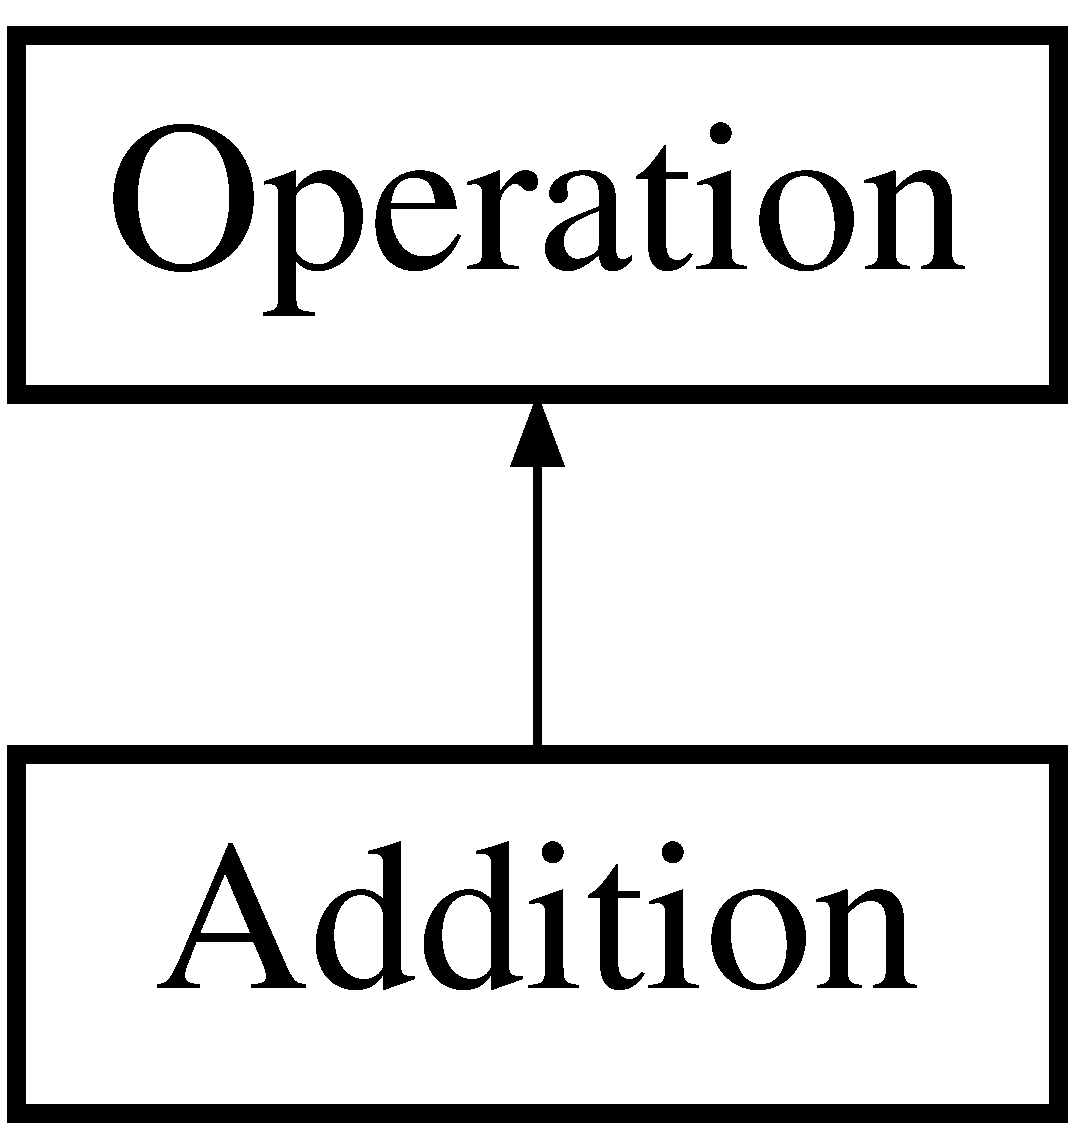
\includegraphics[height=2.000000cm]{classAddition}
\end{center}
\end{figure}
\subsection*{Public Member Functions}
\begin{DoxyCompactItemize}
\item 
int \hyperlink{classAddition_a691bb6b9a2d71d9074254d90389a2713}{get\+\_\+arity} ()\hypertarget{classAddition_a691bb6b9a2d71d9074254d90389a2713}{}\label{classAddition_a691bb6b9a2d71d9074254d90389a2713}

\begin{DoxyCompactList}\small\item\em Returns how many parameters the operation requires. \end{DoxyCompactList}\item 
std\+::string \hyperlink{classAddition_aad65a3e629f302a3fe15327e5259be2f}{get\+\_\+print} ()\hypertarget{classAddition_aad65a3e629f302a3fe15327e5259be2f}{}\label{classAddition_aad65a3e629f302a3fe15327e5259be2f}

\begin{DoxyCompactList}\small\item\em Returns the string representation of the operator. \end{DoxyCompactList}\item 
virtual void \hyperlink{classAddition_a2fe0b74f5aaf992389f39db8e47c671f}{evaluate} (const Eigen\+::\+Array\+X3i \&stack, const Eigen\+::\+Array\+X\+Xd \&x, const Eigen\+::\+Vector\+Xd \&constants, std\+::vector$<$ Eigen\+::\+Array\+X\+Xd $>$ \&buffer, std\+::size\+\_\+t result\+\_\+location)
\begin{DoxyCompactList}\small\item\em evaluates a single command at the location passed in \end{DoxyCompactList}\item 
virtual void \hyperlink{classAddition_a30c3e7495cbe3bdc010f2d3f8570bcc8}{deriv\+\_\+evaluate} (const Eigen\+::\+Array\+X3i \&stack, const int command\+\_\+index, const std\+::vector$<$ Eigen\+::\+Array\+X\+Xd $>$ \&forward\+\_\+buffer, std\+::vector$<$ Eigen\+::\+Array\+X\+Xd $>$ \&reverse\+\_\+buffer, int dependency)
\begin{DoxyCompactList}\small\item\em Computes reverse autodiff partial of a command stack. \end{DoxyCompactList}\end{DoxyCompactItemize}


\subsection{Detailed Description}
This class performs addition. 

\subsection{Member Function Documentation}
\index{Addition@{Addition}!deriv\+\_\+evaluate@{deriv\+\_\+evaluate}}
\index{deriv\+\_\+evaluate@{deriv\+\_\+evaluate}!Addition@{Addition}}
\subsubsection[{\texorpdfstring{deriv\+\_\+evaluate(const Eigen\+::\+Array\+X3i \&stack, const int command\+\_\+index, const std\+::vector$<$ Eigen\+::\+Array\+X\+Xd $>$ \&forward\+\_\+buffer, std\+::vector$<$ Eigen\+::\+Array\+X\+Xd $>$ \&reverse\+\_\+buffer, int dependency)}{deriv_evaluate(const Eigen::ArrayX3i &stack, const int command_index, const std::vector< Eigen::ArrayXXd > &forward_buffer, std::vector< Eigen::ArrayXXd > &reverse_buffer, int dependency)}}]{\setlength{\rightskip}{0pt plus 5cm}void Addition\+::deriv\+\_\+evaluate (
\begin{DoxyParamCaption}
\item[{const Eigen\+::\+Array\+X3i \&}]{stack, }
\item[{const int}]{command\+\_\+index, }
\item[{const std\+::vector$<$ Eigen\+::\+Array\+X\+Xd $>$ \&}]{forward\+\_\+buffer, }
\item[{std\+::vector$<$ Eigen\+::\+Array\+X\+Xd $>$ \&}]{reverse\+\_\+buffer, }
\item[{int}]{dependency}
\end{DoxyParamCaption}
)\hspace{0.3cm}{\ttfamily [virtual]}}\hypertarget{classAddition_a30c3e7495cbe3bdc010f2d3f8570bcc8}{}\label{classAddition_a30c3e7495cbe3bdc010f2d3f8570bcc8}


Computes reverse autodiff partial of a command stack. 


\begin{DoxyParams}[1]{Parameters}
\mbox{\tt in}  & {\em stack} & The stack that contains each command. Eigen\+::\+Array\+X3i \\
\hline
\mbox{\tt in}  & {\em command\+\_\+index} & Index of command in the command; also the location of the result to be placed in the reverse buffer. \\
\hline
\mbox{\tt in}  & {\em forward\+\_\+buffer} & Vector of Eigen arrays for the forward buffer. \\
\hline
 & {\em } & \\
\hline
\end{DoxyParams}


Implements \hyperlink{classOperation_a42b611d08c6b00568c5d1b08688ebcce}{Operation}.

\index{Addition@{Addition}!evaluate@{evaluate}}
\index{evaluate@{evaluate}!Addition@{Addition}}
\subsubsection[{\texorpdfstring{evaluate(const Eigen\+::\+Array\+X3i \&stack, const Eigen\+::\+Array\+X\+Xd \&x, const Eigen\+::\+Vector\+Xd \&constants, std\+::vector$<$ Eigen\+::\+Array\+X\+Xd $>$ \&buffer, std\+::size\+\_\+t result\+\_\+location)}{evaluate(const Eigen::ArrayX3i &stack, const Eigen::ArrayXXd &x, const Eigen::VectorXd &constants, std::vector< Eigen::ArrayXXd > &buffer, std::size_t result_location)}}]{\setlength{\rightskip}{0pt plus 5cm}void Addition\+::evaluate (
\begin{DoxyParamCaption}
\item[{const Eigen\+::\+Array\+X3i \&}]{stack, }
\item[{const Eigen\+::\+Array\+X\+Xd \&}]{x, }
\item[{const Eigen\+::\+Vector\+Xd \&}]{constants, }
\item[{std\+::vector$<$ Eigen\+::\+Array\+X\+Xd $>$ \&}]{buffer, }
\item[{std\+::size\+\_\+t}]{result\+\_\+location}
\end{DoxyParamCaption}
)\hspace{0.3cm}{\ttfamily [virtual]}}\hypertarget{classAddition_a2fe0b74f5aaf992389f39db8e47c671f}{}\label{classAddition_a2fe0b74f5aaf992389f39db8e47c671f}


evaluates a single command at the location passed in 


\begin{DoxyParams}[1]{Parameters}
\mbox{\tt in}  & {\em stack} & The stack that contains each command. Eigen\+::\+Array\+X3i \\
\hline
\mbox{\tt in}  & {\em x} & Input variables to the acyclic graph. Eigen\+::\+Array\+X\+Xd \\
\hline
\mbox{\tt in}  & {\em constants} & Constants used in the command. Eigen\+::\+Vector\+Xd \\
\hline
 & {\em } & \\
\hline
\end{DoxyParams}


Implements \hyperlink{classOperation_a89093eb53f975dd98b6a36d85fa17276}{Operation}.



The documentation for this class was generated from the following files\+:\begin{DoxyCompactItemize}
\item 
/users0/gbomarit/\+Projects/\+Genetic\+\_\+\+Programming/bingo/bingocpp/include/\+Bingo\+Cpp/acyclic\+\_\+graph\+\_\+nodes.\+h\item 
/users0/gbomarit/\+Projects/\+Genetic\+\_\+\+Programming/bingo/bingocpp/src/acyclic\+\_\+graph\+\_\+nodes.\+cpp\end{DoxyCompactItemize}

\hypertarget{classC__Load}{}\section{C\+\_\+\+Load Class Reference}
\label{classC__Load}\index{C\+\_\+\+Load@{C\+\_\+\+Load}}


This class loads the constant.  




{\ttfamily \#include $<$acyclic\+\_\+graph\+\_\+nodes.\+h$>$}

Inheritance diagram for C\+\_\+\+Load\+:\begin{figure}[H]
\begin{center}
\leavevmode
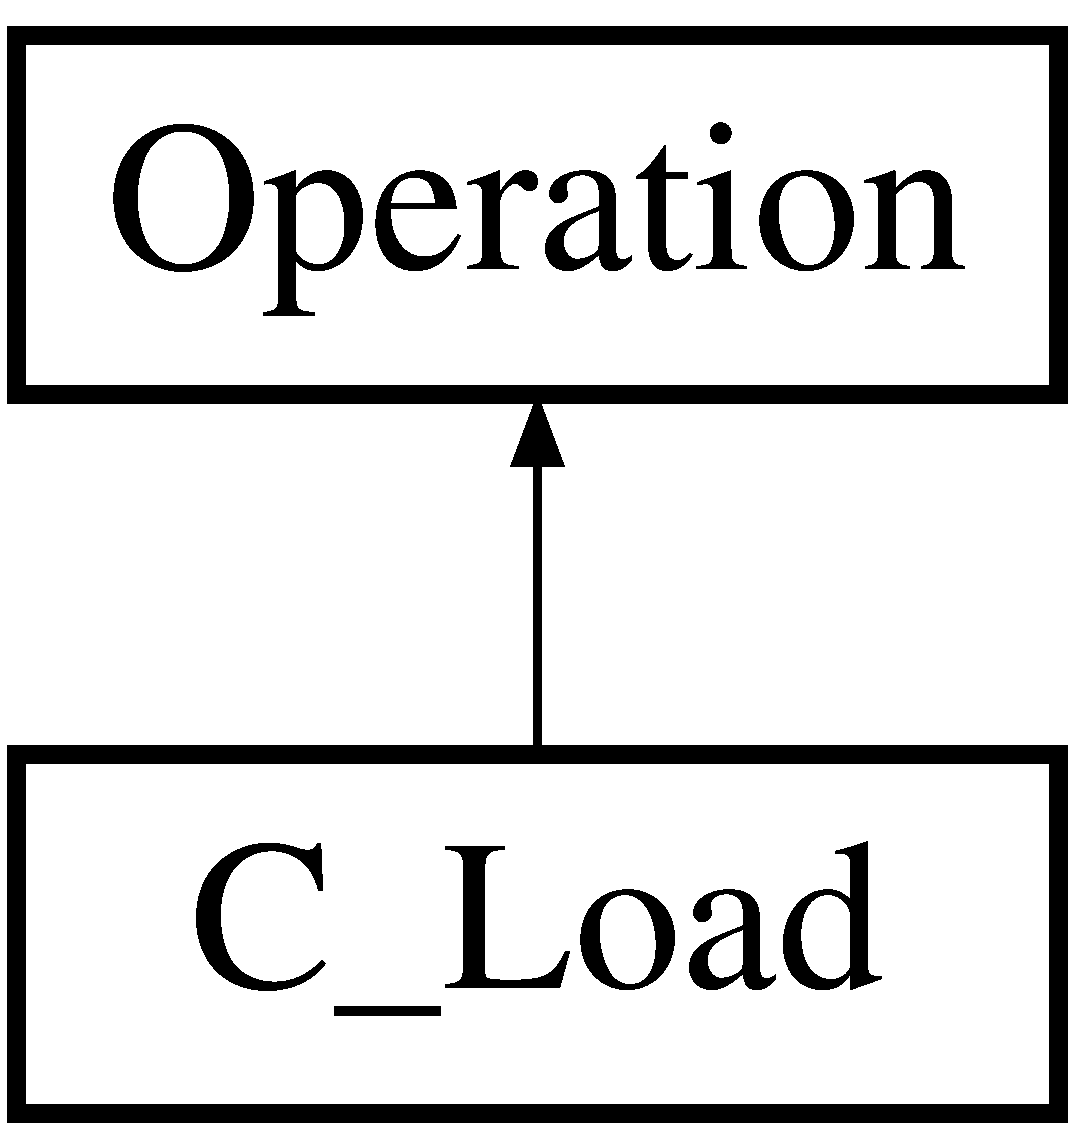
\includegraphics[height=2.000000cm]{classC__Load}
\end{center}
\end{figure}
\subsection*{Public Member Functions}
\begin{DoxyCompactItemize}
\item 
int \hyperlink{classC__Load_ae655fdc171a24965bb5cbb1e2fda9293}{get\+\_\+arity} ()\hypertarget{classC__Load_ae655fdc171a24965bb5cbb1e2fda9293}{}\label{classC__Load_ae655fdc171a24965bb5cbb1e2fda9293}

\begin{DoxyCompactList}\small\item\em Returns how many parameters the operation requires. \end{DoxyCompactList}\item 
std\+::string \hyperlink{classC__Load_a58d4503b40ec02c4da5d5daa1bb51967}{get\+\_\+print} ()\hypertarget{classC__Load_a58d4503b40ec02c4da5d5daa1bb51967}{}\label{classC__Load_a58d4503b40ec02c4da5d5daa1bb51967}

\begin{DoxyCompactList}\small\item\em Returns the string representation of the operator. \end{DoxyCompactList}\item 
virtual void \hyperlink{classC__Load_a82be394b7e177cc378def30ff9972941}{evaluate} (const Eigen\+::\+Array\+X3i \&stack, const Eigen\+::\+Array\+X\+Xd \&x, const Eigen\+::\+Vector\+Xd \&constants, std\+::vector$<$ Eigen\+::\+Array\+X\+Xd $>$ \&buffer, std\+::size\+\_\+t result\+\_\+location)
\begin{DoxyCompactList}\small\item\em evaluates a single command at the location passed in \end{DoxyCompactList}\item 
virtual void \hyperlink{classC__Load_abfe90cef11f940a216284970f6db7b0d}{deriv\+\_\+evaluate} (const Eigen\+::\+Array\+X3i \&stack, const int command\+\_\+index, const std\+::vector$<$ Eigen\+::\+Array\+X\+Xd $>$ \&forward\+\_\+buffer, std\+::vector$<$ Eigen\+::\+Array\+X\+Xd $>$ \&reverse\+\_\+buffer, int dependency)
\begin{DoxyCompactList}\small\item\em Computes reverse autodiff partial of a command stack. \end{DoxyCompactList}\end{DoxyCompactItemize}


\subsection{Detailed Description}
This class loads the constant. 

\subsection{Member Function Documentation}
\index{C\+\_\+\+Load@{C\+\_\+\+Load}!deriv\+\_\+evaluate@{deriv\+\_\+evaluate}}
\index{deriv\+\_\+evaluate@{deriv\+\_\+evaluate}!C\+\_\+\+Load@{C\+\_\+\+Load}}
\subsubsection[{\texorpdfstring{deriv\+\_\+evaluate(const Eigen\+::\+Array\+X3i \&stack, const int command\+\_\+index, const std\+::vector$<$ Eigen\+::\+Array\+X\+Xd $>$ \&forward\+\_\+buffer, std\+::vector$<$ Eigen\+::\+Array\+X\+Xd $>$ \&reverse\+\_\+buffer, int dependency)}{deriv_evaluate(const Eigen::ArrayX3i &stack, const int command_index, const std::vector< Eigen::ArrayXXd > &forward_buffer, std::vector< Eigen::ArrayXXd > &reverse_buffer, int dependency)}}]{\setlength{\rightskip}{0pt plus 5cm}void C\+\_\+\+Load\+::deriv\+\_\+evaluate (
\begin{DoxyParamCaption}
\item[{const Eigen\+::\+Array\+X3i \&}]{stack, }
\item[{const int}]{command\+\_\+index, }
\item[{const std\+::vector$<$ Eigen\+::\+Array\+X\+Xd $>$ \&}]{forward\+\_\+buffer, }
\item[{std\+::vector$<$ Eigen\+::\+Array\+X\+Xd $>$ \&}]{reverse\+\_\+buffer, }
\item[{int}]{dependency}
\end{DoxyParamCaption}
)\hspace{0.3cm}{\ttfamily [virtual]}}\hypertarget{classC__Load_abfe90cef11f940a216284970f6db7b0d}{}\label{classC__Load_abfe90cef11f940a216284970f6db7b0d}


Computes reverse autodiff partial of a command stack. 


\begin{DoxyParams}[1]{Parameters}
\mbox{\tt in}  & {\em stack} & The stack that contains each command. Eigen\+::\+Array\+X3i \\
\hline
\mbox{\tt in}  & {\em command\+\_\+index} & Index of command in the command; also the location of the result to be placed in the reverse buffer. \\
\hline
\mbox{\tt in}  & {\em forward\+\_\+buffer} & Vector of Eigen arrays for the forward buffer. \\
\hline
 & {\em } & \\
\hline
\end{DoxyParams}


Implements \hyperlink{classOperation_a42b611d08c6b00568c5d1b08688ebcce}{Operation}.

\index{C\+\_\+\+Load@{C\+\_\+\+Load}!evaluate@{evaluate}}
\index{evaluate@{evaluate}!C\+\_\+\+Load@{C\+\_\+\+Load}}
\subsubsection[{\texorpdfstring{evaluate(const Eigen\+::\+Array\+X3i \&stack, const Eigen\+::\+Array\+X\+Xd \&x, const Eigen\+::\+Vector\+Xd \&constants, std\+::vector$<$ Eigen\+::\+Array\+X\+Xd $>$ \&buffer, std\+::size\+\_\+t result\+\_\+location)}{evaluate(const Eigen::ArrayX3i &stack, const Eigen::ArrayXXd &x, const Eigen::VectorXd &constants, std::vector< Eigen::ArrayXXd > &buffer, std::size_t result_location)}}]{\setlength{\rightskip}{0pt plus 5cm}void C\+\_\+\+Load\+::evaluate (
\begin{DoxyParamCaption}
\item[{const Eigen\+::\+Array\+X3i \&}]{stack, }
\item[{const Eigen\+::\+Array\+X\+Xd \&}]{x, }
\item[{const Eigen\+::\+Vector\+Xd \&}]{constants, }
\item[{std\+::vector$<$ Eigen\+::\+Array\+X\+Xd $>$ \&}]{buffer, }
\item[{std\+::size\+\_\+t}]{result\+\_\+location}
\end{DoxyParamCaption}
)\hspace{0.3cm}{\ttfamily [virtual]}}\hypertarget{classC__Load_a82be394b7e177cc378def30ff9972941}{}\label{classC__Load_a82be394b7e177cc378def30ff9972941}


evaluates a single command at the location passed in 


\begin{DoxyParams}[1]{Parameters}
\mbox{\tt in}  & {\em stack} & The stack that contains each command. Eigen\+::\+Array\+X3i \\
\hline
\mbox{\tt in}  & {\em x} & Input variables to the acyclic graph. Eigen\+::\+Array\+X\+Xd \\
\hline
\mbox{\tt in}  & {\em constants} & Constants used in the command. Eigen\+::\+Vector\+Xd \\
\hline
 & {\em } & \\
\hline
\end{DoxyParams}


Implements \hyperlink{classOperation_a89093eb53f975dd98b6a36d85fa17276}{Operation}.



The documentation for this class was generated from the following files\+:\begin{DoxyCompactItemize}
\item 
/users0/gbomarit/\+Projects/\+Genetic\+\_\+\+Programming/bingo/bingocpp/include/\+Bingo\+Cpp/acyclic\+\_\+graph\+\_\+nodes.\+h\item 
/users0/gbomarit/\+Projects/\+Genetic\+\_\+\+Programming/bingo/bingocpp/src/acyclic\+\_\+graph\+\_\+nodes.\+cpp\end{DoxyCompactItemize}

\hypertarget{classCos}{}\section{Cos Class Reference}
\label{classCos}\index{Cos@{Cos}}


This class performs cosine.  




{\ttfamily \#include $<$acyclic\+\_\+graph\+\_\+nodes.\+h$>$}

Inheritance diagram for Cos\+:\begin{figure}[H]
\begin{center}
\leavevmode
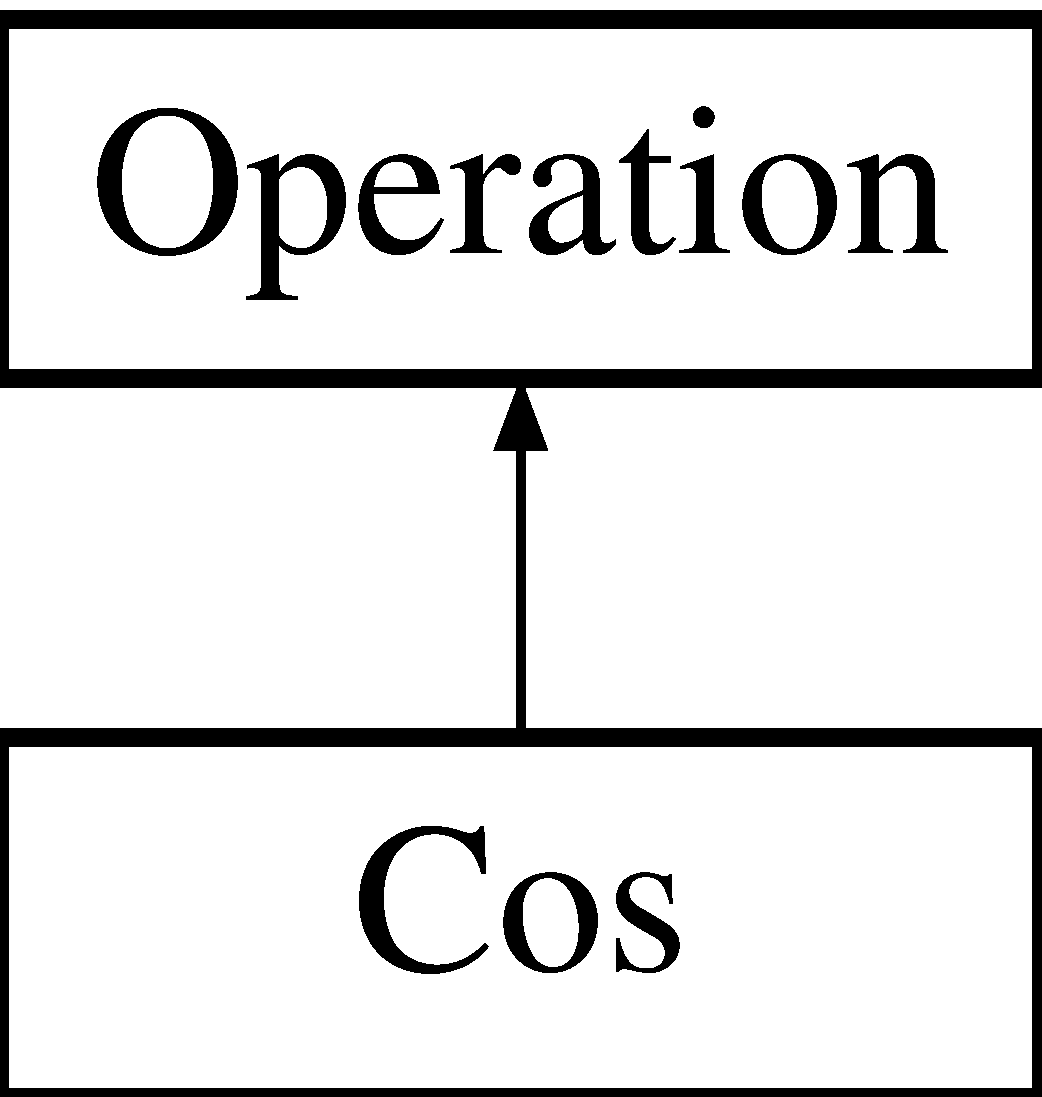
\includegraphics[height=2.000000cm]{classCos}
\end{center}
\end{figure}
\subsection*{Public Member Functions}
\begin{DoxyCompactItemize}
\item 
int \hyperlink{classCos_ac2beebc68e2983e2f6f27728c04d32b8}{get\+\_\+arity} ()\hypertarget{classCos_ac2beebc68e2983e2f6f27728c04d32b8}{}\label{classCos_ac2beebc68e2983e2f6f27728c04d32b8}

\begin{DoxyCompactList}\small\item\em Returns how many parameters the operation requires. \end{DoxyCompactList}\item 
std\+::string \hyperlink{classCos_a4db275037edc252704370b203dcc2efb}{get\+\_\+print} ()\hypertarget{classCos_a4db275037edc252704370b203dcc2efb}{}\label{classCos_a4db275037edc252704370b203dcc2efb}

\begin{DoxyCompactList}\small\item\em Returns the string representation of the operator. \end{DoxyCompactList}\item 
virtual void \hyperlink{classCos_a580742a5758d0e31ecfc98c9e49fa597}{evaluate} (const Eigen\+::\+Array\+X3i \&stack, const Eigen\+::\+Array\+X\+Xd \&x, const Eigen\+::\+Vector\+Xd \&constants, std\+::vector$<$ Eigen\+::\+Array\+X\+Xd $>$ \&buffer, std\+::size\+\_\+t result\+\_\+location)
\begin{DoxyCompactList}\small\item\em evaluates a single command at the location passed in \end{DoxyCompactList}\item 
virtual void \hyperlink{classCos_a4ca2ae643db43a16772f9fdbb86c06a6}{deriv\+\_\+evaluate} (const Eigen\+::\+Array\+X3i \&stack, const int command\+\_\+index, const std\+::vector$<$ Eigen\+::\+Array\+X\+Xd $>$ \&forward\+\_\+buffer, std\+::vector$<$ Eigen\+::\+Array\+X\+Xd $>$ \&reverse\+\_\+buffer, int dependency)
\begin{DoxyCompactList}\small\item\em Computes reverse autodiff partial of a command stack. \end{DoxyCompactList}\end{DoxyCompactItemize}


\subsection{Detailed Description}
This class performs cosine. 

\subsection{Member Function Documentation}
\index{Cos@{Cos}!deriv\+\_\+evaluate@{deriv\+\_\+evaluate}}
\index{deriv\+\_\+evaluate@{deriv\+\_\+evaluate}!Cos@{Cos}}
\subsubsection[{\texorpdfstring{deriv\+\_\+evaluate(const Eigen\+::\+Array\+X3i \&stack, const int command\+\_\+index, const std\+::vector$<$ Eigen\+::\+Array\+X\+Xd $>$ \&forward\+\_\+buffer, std\+::vector$<$ Eigen\+::\+Array\+X\+Xd $>$ \&reverse\+\_\+buffer, int dependency)}{deriv_evaluate(const Eigen::ArrayX3i &stack, const int command_index, const std::vector< Eigen::ArrayXXd > &forward_buffer, std::vector< Eigen::ArrayXXd > &reverse_buffer, int dependency)}}]{\setlength{\rightskip}{0pt plus 5cm}void Cos\+::deriv\+\_\+evaluate (
\begin{DoxyParamCaption}
\item[{const Eigen\+::\+Array\+X3i \&}]{stack, }
\item[{const int}]{command\+\_\+index, }
\item[{const std\+::vector$<$ Eigen\+::\+Array\+X\+Xd $>$ \&}]{forward\+\_\+buffer, }
\item[{std\+::vector$<$ Eigen\+::\+Array\+X\+Xd $>$ \&}]{reverse\+\_\+buffer, }
\item[{int}]{dependency}
\end{DoxyParamCaption}
)\hspace{0.3cm}{\ttfamily [virtual]}}\hypertarget{classCos_a4ca2ae643db43a16772f9fdbb86c06a6}{}\label{classCos_a4ca2ae643db43a16772f9fdbb86c06a6}


Computes reverse autodiff partial of a command stack. 


\begin{DoxyParams}[1]{Parameters}
\mbox{\tt in}  & {\em stack} & The stack that contains each command. Eigen\+::\+Array\+X3i \\
\hline
\mbox{\tt in}  & {\em command\+\_\+index} & Index of command in the command; also the location of the result to be placed in the reverse buffer. \\
\hline
\mbox{\tt in}  & {\em forward\+\_\+buffer} & Vector of Eigen arrays for the forward buffer. \\
\hline
 & {\em } & \\
\hline
\end{DoxyParams}


Implements \hyperlink{classOperation_a42b611d08c6b00568c5d1b08688ebcce}{Operation}.

\index{Cos@{Cos}!evaluate@{evaluate}}
\index{evaluate@{evaluate}!Cos@{Cos}}
\subsubsection[{\texorpdfstring{evaluate(const Eigen\+::\+Array\+X3i \&stack, const Eigen\+::\+Array\+X\+Xd \&x, const Eigen\+::\+Vector\+Xd \&constants, std\+::vector$<$ Eigen\+::\+Array\+X\+Xd $>$ \&buffer, std\+::size\+\_\+t result\+\_\+location)}{evaluate(const Eigen::ArrayX3i &stack, const Eigen::ArrayXXd &x, const Eigen::VectorXd &constants, std::vector< Eigen::ArrayXXd > &buffer, std::size_t result_location)}}]{\setlength{\rightskip}{0pt plus 5cm}void Cos\+::evaluate (
\begin{DoxyParamCaption}
\item[{const Eigen\+::\+Array\+X3i \&}]{stack, }
\item[{const Eigen\+::\+Array\+X\+Xd \&}]{x, }
\item[{const Eigen\+::\+Vector\+Xd \&}]{constants, }
\item[{std\+::vector$<$ Eigen\+::\+Array\+X\+Xd $>$ \&}]{buffer, }
\item[{std\+::size\+\_\+t}]{result\+\_\+location}
\end{DoxyParamCaption}
)\hspace{0.3cm}{\ttfamily [virtual]}}\hypertarget{classCos_a580742a5758d0e31ecfc98c9e49fa597}{}\label{classCos_a580742a5758d0e31ecfc98c9e49fa597}


evaluates a single command at the location passed in 


\begin{DoxyParams}[1]{Parameters}
\mbox{\tt in}  & {\em stack} & The stack that contains each command. Eigen\+::\+Array\+X3i \\
\hline
\mbox{\tt in}  & {\em x} & Input variables to the acyclic graph. Eigen\+::\+Array\+X\+Xd \\
\hline
\mbox{\tt in}  & {\em constants} & Constants used in the command. Eigen\+::\+Vector\+Xd \\
\hline
 & {\em } & \\
\hline
\end{DoxyParams}


Implements \hyperlink{classOperation_a89093eb53f975dd98b6a36d85fa17276}{Operation}.



The documentation for this class was generated from the following files\+:\begin{DoxyCompactItemize}
\item 
/users0/gbomarit/\+Projects/\+Genetic\+\_\+\+Programming/bingo/bingocpp/include/\+Bingo\+Cpp/acyclic\+\_\+graph\+\_\+nodes.\+h\item 
/users0/gbomarit/\+Projects/\+Genetic\+\_\+\+Programming/bingo/bingocpp/src/acyclic\+\_\+graph\+\_\+nodes.\+cpp\end{DoxyCompactItemize}

\hypertarget{classDivision}{}\section{Division Class Reference}
\label{classDivision}\index{Division@{Division}}


This class performs division.  




{\ttfamily \#include $<$acyclic\+\_\+graph\+\_\+nodes.\+h$>$}

Inheritance diagram for Division\+:\begin{figure}[H]
\begin{center}
\leavevmode
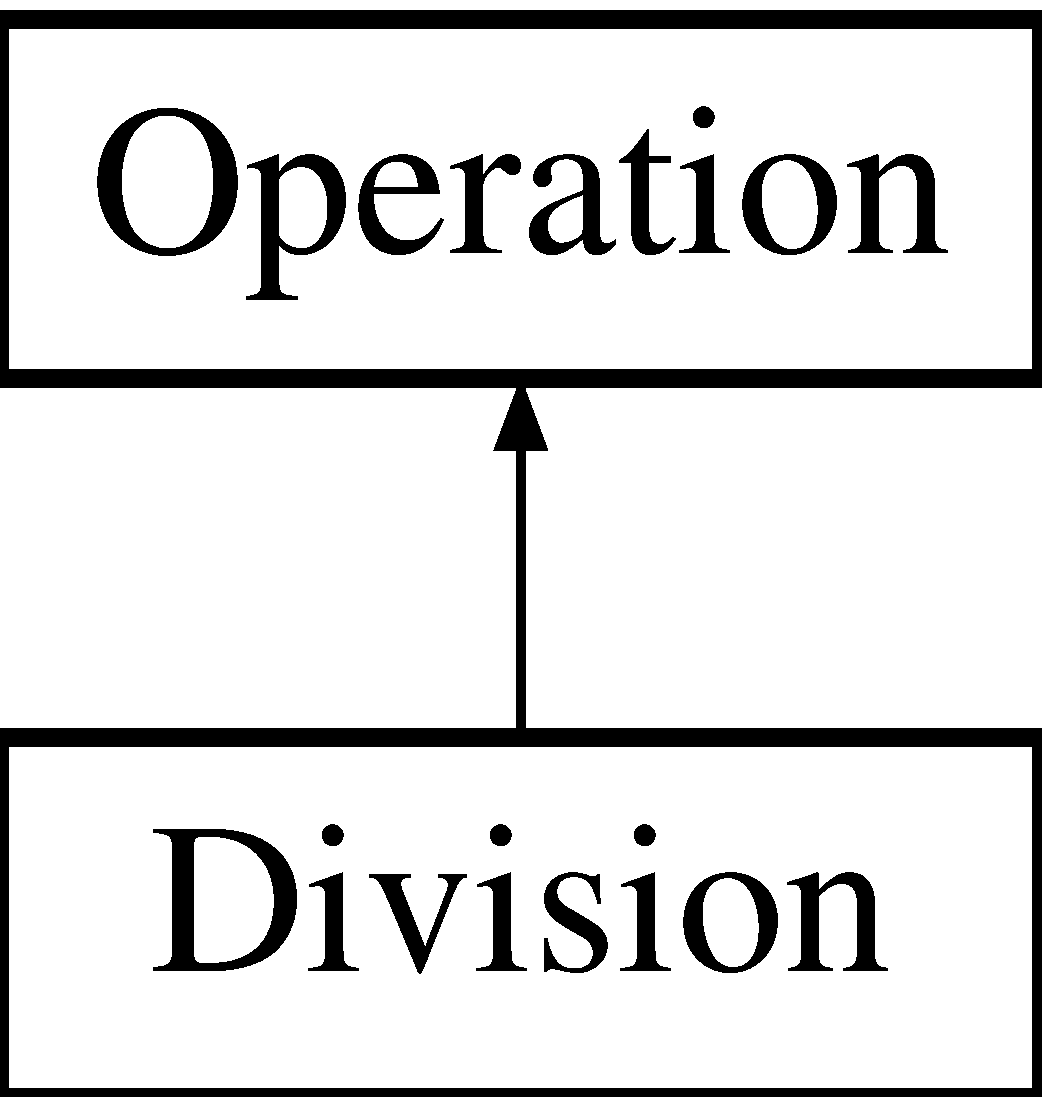
\includegraphics[height=2.000000cm]{classDivision}
\end{center}
\end{figure}
\subsection*{Public Member Functions}
\begin{DoxyCompactItemize}
\item 
int \hyperlink{classDivision_a269601e11e98c4fc5f885363b9c8a2c5}{get\+\_\+arity} ()\hypertarget{classDivision_a269601e11e98c4fc5f885363b9c8a2c5}{}\label{classDivision_a269601e11e98c4fc5f885363b9c8a2c5}

\begin{DoxyCompactList}\small\item\em Returns how many parameters the operation requires. \end{DoxyCompactList}\item 
std\+::string \hyperlink{classDivision_a05bf2f19700b47d772be822f85aeb884}{get\+\_\+print} ()\hypertarget{classDivision_a05bf2f19700b47d772be822f85aeb884}{}\label{classDivision_a05bf2f19700b47d772be822f85aeb884}

\begin{DoxyCompactList}\small\item\em Returns the string representation of the operator. \end{DoxyCompactList}\item 
virtual void \hyperlink{classDivision_a09bcc06557768b3a3abc31667ab03103}{evaluate} (const Eigen\+::\+Array\+X3i \&stack, const Eigen\+::\+Array\+X\+Xd \&x, const Eigen\+::\+Vector\+Xd \&constants, std\+::vector$<$ Eigen\+::\+Array\+X\+Xd $>$ \&buffer, std\+::size\+\_\+t result\+\_\+location)
\begin{DoxyCompactList}\small\item\em evaluates a single command at the location passed in \end{DoxyCompactList}\item 
virtual void \hyperlink{classDivision_af0f88f306718e3a490315e4be78885f3}{deriv\+\_\+evaluate} (const Eigen\+::\+Array\+X3i \&stack, const int command\+\_\+index, const std\+::vector$<$ Eigen\+::\+Array\+X\+Xd $>$ \&forward\+\_\+buffer, std\+::vector$<$ Eigen\+::\+Array\+X\+Xd $>$ \&reverse\+\_\+buffer, int dependency)
\begin{DoxyCompactList}\small\item\em Computes reverse autodiff partial of a command stack. \end{DoxyCompactList}\end{DoxyCompactItemize}


\subsection{Detailed Description}
This class performs division. 

\subsection{Member Function Documentation}
\index{Division@{Division}!deriv\+\_\+evaluate@{deriv\+\_\+evaluate}}
\index{deriv\+\_\+evaluate@{deriv\+\_\+evaluate}!Division@{Division}}
\subsubsection[{\texorpdfstring{deriv\+\_\+evaluate(const Eigen\+::\+Array\+X3i \&stack, const int command\+\_\+index, const std\+::vector$<$ Eigen\+::\+Array\+X\+Xd $>$ \&forward\+\_\+buffer, std\+::vector$<$ Eigen\+::\+Array\+X\+Xd $>$ \&reverse\+\_\+buffer, int dependency)}{deriv_evaluate(const Eigen::ArrayX3i &stack, const int command_index, const std::vector< Eigen::ArrayXXd > &forward_buffer, std::vector< Eigen::ArrayXXd > &reverse_buffer, int dependency)}}]{\setlength{\rightskip}{0pt plus 5cm}void Division\+::deriv\+\_\+evaluate (
\begin{DoxyParamCaption}
\item[{const Eigen\+::\+Array\+X3i \&}]{stack, }
\item[{const int}]{command\+\_\+index, }
\item[{const std\+::vector$<$ Eigen\+::\+Array\+X\+Xd $>$ \&}]{forward\+\_\+buffer, }
\item[{std\+::vector$<$ Eigen\+::\+Array\+X\+Xd $>$ \&}]{reverse\+\_\+buffer, }
\item[{int}]{dependency}
\end{DoxyParamCaption}
)\hspace{0.3cm}{\ttfamily [virtual]}}\hypertarget{classDivision_af0f88f306718e3a490315e4be78885f3}{}\label{classDivision_af0f88f306718e3a490315e4be78885f3}


Computes reverse autodiff partial of a command stack. 


\begin{DoxyParams}[1]{Parameters}
\mbox{\tt in}  & {\em stack} & The stack that contains each command. Eigen\+::\+Array\+X3i \\
\hline
\mbox{\tt in}  & {\em command\+\_\+index} & Index of command in the command; also the location of the result to be placed in the reverse buffer. \\
\hline
\mbox{\tt in}  & {\em forward\+\_\+buffer} & Vector of Eigen arrays for the forward buffer. \\
\hline
 & {\em } & \\
\hline
\end{DoxyParams}


Implements \hyperlink{classOperation_a42b611d08c6b00568c5d1b08688ebcce}{Operation}.

\index{Division@{Division}!evaluate@{evaluate}}
\index{evaluate@{evaluate}!Division@{Division}}
\subsubsection[{\texorpdfstring{evaluate(const Eigen\+::\+Array\+X3i \&stack, const Eigen\+::\+Array\+X\+Xd \&x, const Eigen\+::\+Vector\+Xd \&constants, std\+::vector$<$ Eigen\+::\+Array\+X\+Xd $>$ \&buffer, std\+::size\+\_\+t result\+\_\+location)}{evaluate(const Eigen::ArrayX3i &stack, const Eigen::ArrayXXd &x, const Eigen::VectorXd &constants, std::vector< Eigen::ArrayXXd > &buffer, std::size_t result_location)}}]{\setlength{\rightskip}{0pt plus 5cm}void Division\+::evaluate (
\begin{DoxyParamCaption}
\item[{const Eigen\+::\+Array\+X3i \&}]{stack, }
\item[{const Eigen\+::\+Array\+X\+Xd \&}]{x, }
\item[{const Eigen\+::\+Vector\+Xd \&}]{constants, }
\item[{std\+::vector$<$ Eigen\+::\+Array\+X\+Xd $>$ \&}]{buffer, }
\item[{std\+::size\+\_\+t}]{result\+\_\+location}
\end{DoxyParamCaption}
)\hspace{0.3cm}{\ttfamily [virtual]}}\hypertarget{classDivision_a09bcc06557768b3a3abc31667ab03103}{}\label{classDivision_a09bcc06557768b3a3abc31667ab03103}


evaluates a single command at the location passed in 


\begin{DoxyParams}[1]{Parameters}
\mbox{\tt in}  & {\em stack} & The stack that contains each command. Eigen\+::\+Array\+X3i \\
\hline
\mbox{\tt in}  & {\em x} & Input variables to the acyclic graph. Eigen\+::\+Array\+X\+Xd \\
\hline
\mbox{\tt in}  & {\em constants} & Constants used in the command. Eigen\+::\+Vector\+Xd \\
\hline
 & {\em } & \\
\hline
\end{DoxyParams}


Implements \hyperlink{classOperation_a89093eb53f975dd98b6a36d85fa17276}{Operation}.



The documentation for this class was generated from the following files\+:\begin{DoxyCompactItemize}
\item 
/users0/gbomarit/\+Projects/\+Genetic\+\_\+\+Programming/bingo/bingocpp/include/\+Bingo\+Cpp/acyclic\+\_\+graph\+\_\+nodes.\+h\item 
/users0/gbomarit/\+Projects/\+Genetic\+\_\+\+Programming/bingo/bingocpp/src/acyclic\+\_\+graph\+\_\+nodes.\+cpp\end{DoxyCompactItemize}

\hypertarget{classExp}{}\section{Exp Class Reference}
\label{classExp}\index{Exp@{Exp}}


This class performs an exponential.  




{\ttfamily \#include $<$acyclic\+\_\+graph\+\_\+nodes.\+h$>$}

Inheritance diagram for Exp\+:\begin{figure}[H]
\begin{center}
\leavevmode
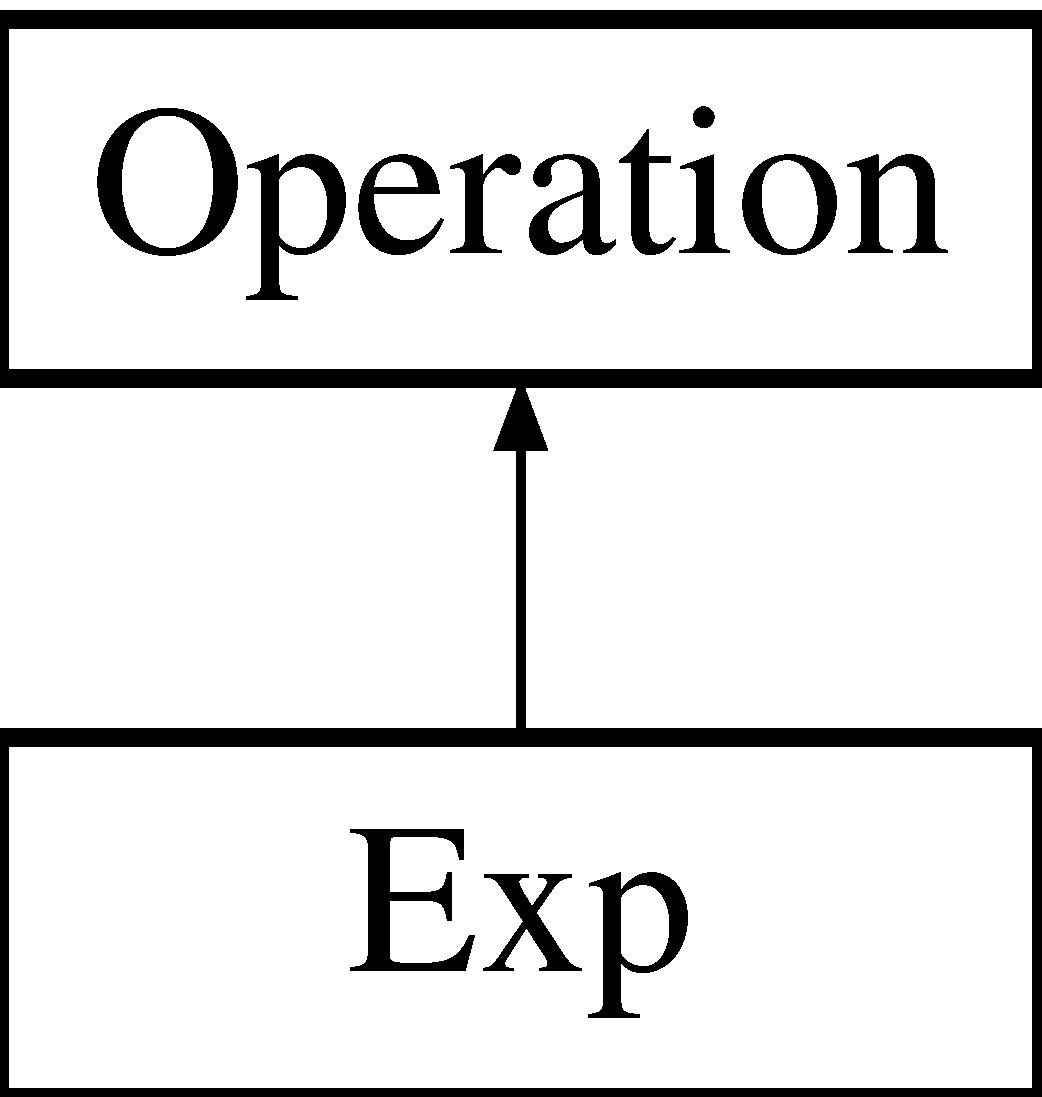
\includegraphics[height=2.000000cm]{classExp}
\end{center}
\end{figure}
\subsection*{Public Member Functions}
\begin{DoxyCompactItemize}
\item 
int \hyperlink{classExp_a4174a935068765b990ab706e7ec1bbbe}{get\+\_\+arity} ()\hypertarget{classExp_a4174a935068765b990ab706e7ec1bbbe}{}\label{classExp_a4174a935068765b990ab706e7ec1bbbe}

\begin{DoxyCompactList}\small\item\em Returns how many parameters the operation requires. \end{DoxyCompactList}\item 
std\+::string \hyperlink{classExp_a591369485b6ce08f11132ca81225d0d4}{get\+\_\+print} ()\hypertarget{classExp_a591369485b6ce08f11132ca81225d0d4}{}\label{classExp_a591369485b6ce08f11132ca81225d0d4}

\begin{DoxyCompactList}\small\item\em Returns the string representation of the operator. \end{DoxyCompactList}\item 
virtual void \hyperlink{classExp_a12142e937f2fa11002ebe3d574626aa5}{evaluate} (const Eigen\+::\+Array\+X3i \&stack, const Eigen\+::\+Array\+X\+Xd \&x, const Eigen\+::\+Vector\+Xd \&constants, std\+::vector$<$ Eigen\+::\+Array\+X\+Xd $>$ \&buffer, std\+::size\+\_\+t result\+\_\+location)
\begin{DoxyCompactList}\small\item\em evaluates a single command at the location passed in \end{DoxyCompactList}\item 
virtual void \hyperlink{classExp_aaf9e4870dcd8eda83174f003d9bd4a8a}{deriv\+\_\+evaluate} (const Eigen\+::\+Array\+X3i \&stack, const int command\+\_\+index, const std\+::vector$<$ Eigen\+::\+Array\+X\+Xd $>$ \&forward\+\_\+buffer, std\+::vector$<$ Eigen\+::\+Array\+X\+Xd $>$ \&reverse\+\_\+buffer, int dependency)
\begin{DoxyCompactList}\small\item\em Computes reverse autodiff partial of a command stack. \end{DoxyCompactList}\end{DoxyCompactItemize}


\subsection{Detailed Description}
This class performs an exponential. 

\subsection{Member Function Documentation}
\index{Exp@{Exp}!deriv\+\_\+evaluate@{deriv\+\_\+evaluate}}
\index{deriv\+\_\+evaluate@{deriv\+\_\+evaluate}!Exp@{Exp}}
\subsubsection[{\texorpdfstring{deriv\+\_\+evaluate(const Eigen\+::\+Array\+X3i \&stack, const int command\+\_\+index, const std\+::vector$<$ Eigen\+::\+Array\+X\+Xd $>$ \&forward\+\_\+buffer, std\+::vector$<$ Eigen\+::\+Array\+X\+Xd $>$ \&reverse\+\_\+buffer, int dependency)}{deriv_evaluate(const Eigen::ArrayX3i &stack, const int command_index, const std::vector< Eigen::ArrayXXd > &forward_buffer, std::vector< Eigen::ArrayXXd > &reverse_buffer, int dependency)}}]{\setlength{\rightskip}{0pt plus 5cm}void Exp\+::deriv\+\_\+evaluate (
\begin{DoxyParamCaption}
\item[{const Eigen\+::\+Array\+X3i \&}]{stack, }
\item[{const int}]{command\+\_\+index, }
\item[{const std\+::vector$<$ Eigen\+::\+Array\+X\+Xd $>$ \&}]{forward\+\_\+buffer, }
\item[{std\+::vector$<$ Eigen\+::\+Array\+X\+Xd $>$ \&}]{reverse\+\_\+buffer, }
\item[{int}]{dependency}
\end{DoxyParamCaption}
)\hspace{0.3cm}{\ttfamily [virtual]}}\hypertarget{classExp_aaf9e4870dcd8eda83174f003d9bd4a8a}{}\label{classExp_aaf9e4870dcd8eda83174f003d9bd4a8a}


Computes reverse autodiff partial of a command stack. 


\begin{DoxyParams}[1]{Parameters}
\mbox{\tt in}  & {\em stack} & The stack that contains each command. Eigen\+::\+Array\+X3i \\
\hline
\mbox{\tt in}  & {\em command\+\_\+index} & Index of command in the command; also the location of the result to be placed in the reverse buffer. \\
\hline
\mbox{\tt in}  & {\em forward\+\_\+buffer} & Vector of Eigen arrays for the forward buffer. \\
\hline
 & {\em } & \\
\hline
\end{DoxyParams}


Implements \hyperlink{classOperation_a42b611d08c6b00568c5d1b08688ebcce}{Operation}.

\index{Exp@{Exp}!evaluate@{evaluate}}
\index{evaluate@{evaluate}!Exp@{Exp}}
\subsubsection[{\texorpdfstring{evaluate(const Eigen\+::\+Array\+X3i \&stack, const Eigen\+::\+Array\+X\+Xd \&x, const Eigen\+::\+Vector\+Xd \&constants, std\+::vector$<$ Eigen\+::\+Array\+X\+Xd $>$ \&buffer, std\+::size\+\_\+t result\+\_\+location)}{evaluate(const Eigen::ArrayX3i &stack, const Eigen::ArrayXXd &x, const Eigen::VectorXd &constants, std::vector< Eigen::ArrayXXd > &buffer, std::size_t result_location)}}]{\setlength{\rightskip}{0pt plus 5cm}void Exp\+::evaluate (
\begin{DoxyParamCaption}
\item[{const Eigen\+::\+Array\+X3i \&}]{stack, }
\item[{const Eigen\+::\+Array\+X\+Xd \&}]{x, }
\item[{const Eigen\+::\+Vector\+Xd \&}]{constants, }
\item[{std\+::vector$<$ Eigen\+::\+Array\+X\+Xd $>$ \&}]{buffer, }
\item[{std\+::size\+\_\+t}]{result\+\_\+location}
\end{DoxyParamCaption}
)\hspace{0.3cm}{\ttfamily [virtual]}}\hypertarget{classExp_a12142e937f2fa11002ebe3d574626aa5}{}\label{classExp_a12142e937f2fa11002ebe3d574626aa5}


evaluates a single command at the location passed in 


\begin{DoxyParams}[1]{Parameters}
\mbox{\tt in}  & {\em stack} & The stack that contains each command. Eigen\+::\+Array\+X3i \\
\hline
\mbox{\tt in}  & {\em x} & Input variables to the acyclic graph. Eigen\+::\+Array\+X\+Xd \\
\hline
\mbox{\tt in}  & {\em constants} & Constants used in the command. Eigen\+::\+Vector\+Xd \\
\hline
 & {\em } & \\
\hline
\end{DoxyParams}


Implements \hyperlink{classOperation_a89093eb53f975dd98b6a36d85fa17276}{Operation}.



The documentation for this class was generated from the following files\+:\begin{DoxyCompactItemize}
\item 
/users0/gbomarit/\+Projects/\+Genetic\+\_\+\+Programming/bingo/bingocpp/include/\+Bingo\+Cpp/acyclic\+\_\+graph\+\_\+nodes.\+h\item 
/users0/gbomarit/\+Projects/\+Genetic\+\_\+\+Programming/bingo/bingocpp/src/acyclic\+\_\+graph\+\_\+nodes.\+cpp\end{DoxyCompactItemize}

\hypertarget{structExplicitTrainingData}{}\section{Explicit\+Training\+Data Struct Reference}
\label{structExplicitTrainingData}\index{Explicit\+Training\+Data@{Explicit\+Training\+Data}}


This struct holds data for Explicit regression.  




{\ttfamily \#include $<$training\+\_\+data.\+h$>$}

Inheritance diagram for Explicit\+Training\+Data\+:\begin{figure}[H]
\begin{center}
\leavevmode
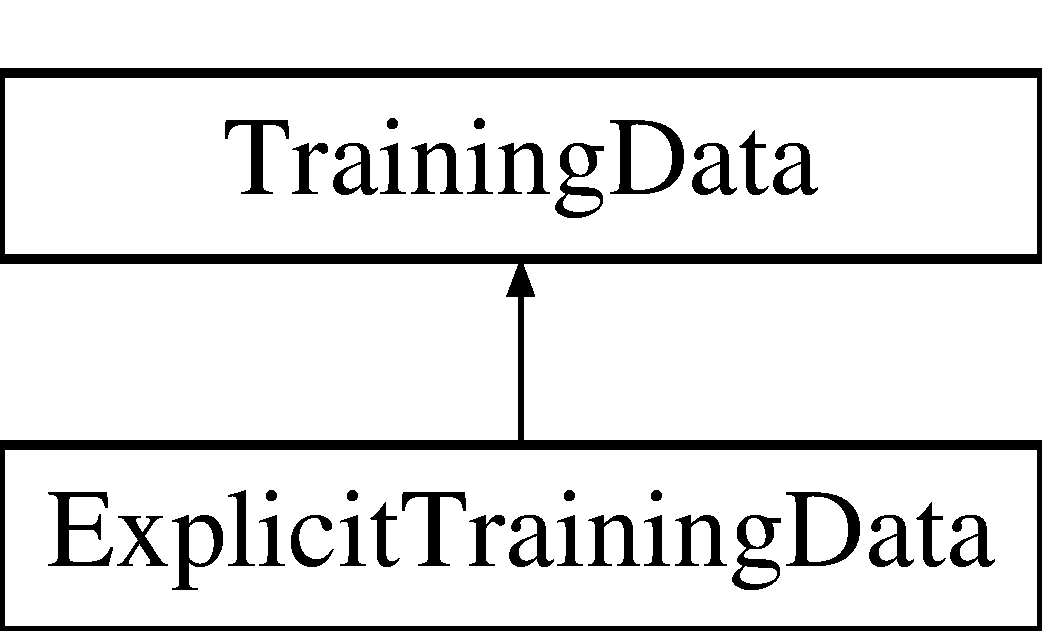
\includegraphics[height=2.000000cm]{structExplicitTrainingData}
\end{center}
\end{figure}
\subsection*{Public Member Functions}
\begin{DoxyCompactItemize}
\item 
\hyperlink{structExplicitTrainingData_a96eb847c22542ecc3f60201d36935e39}{Explicit\+Training\+Data} (Eigen\+::\+Array\+X\+Xd vx, Eigen\+::\+Array\+X\+Xd vy)\hypertarget{structExplicitTrainingData_a96eb847c22542ecc3f60201d36935e39}{}\label{structExplicitTrainingData_a96eb847c22542ecc3f60201d36935e39}

\begin{DoxyCompactList}\small\item\em Constructor. \end{DoxyCompactList}\item 
\hyperlink{structExplicitTrainingData}{Explicit\+Training\+Data} $\ast$ \hyperlink{structExplicitTrainingData_a7c60c1b5ea185580a5842c5cca18c7d0}{get\+\_\+item} (std\+::list$<$ int $>$ items)
\begin{DoxyCompactList}\small\item\em gets a new training data with certain rows \end{DoxyCompactList}\item 
int \hyperlink{structExplicitTrainingData_aa5a3da99babf2436bdb9b4652a217584}{size} ()
\begin{DoxyCompactList}\small\item\em gets the size of x \end{DoxyCompactList}\end{DoxyCompactItemize}
\subsection*{Public Attributes}
\begin{DoxyCompactItemize}
\item 
Eigen\+::\+Array\+X\+Xd \hyperlink{structExplicitTrainingData_aff442821da57c0cf21ab4f2a7396c7e8}{x}
\begin{DoxyCompactList}\small\item\em Eigen\+::\+Array\+X\+Xd x. \end{DoxyCompactList}\item 
Eigen\+::\+Array\+X\+Xd \hyperlink{structExplicitTrainingData_a0a1ca87e118aa4261a910b54cf29d0ee}{y}
\begin{DoxyCompactList}\small\item\em Eigen\+::\+Array\+X\+Xd y. \end{DoxyCompactList}\end{DoxyCompactItemize}


\subsection{Detailed Description}
This struct holds data for Explicit regression. 

\subsection{Member Function Documentation}
\index{Explicit\+Training\+Data@{Explicit\+Training\+Data}!get\+\_\+item@{get\+\_\+item}}
\index{get\+\_\+item@{get\+\_\+item}!Explicit\+Training\+Data@{Explicit\+Training\+Data}}
\subsubsection[{\texorpdfstring{get\+\_\+item(std\+::list$<$ int $>$ items)}{get_item(std::list< int > items)}}]{\setlength{\rightskip}{0pt plus 5cm}{\bf Explicit\+Training\+Data} $\ast$ Explicit\+Training\+Data\+::get\+\_\+item (
\begin{DoxyParamCaption}
\item[{std\+::list$<$ int $>$}]{items}
\end{DoxyParamCaption}
)\hspace{0.3cm}{\ttfamily [virtual]}}\hypertarget{structExplicitTrainingData_a7c60c1b5ea185580a5842c5cca18c7d0}{}\label{structExplicitTrainingData_a7c60c1b5ea185580a5842c5cca18c7d0}


gets a new training data with certain rows 


\begin{DoxyParams}[1]{Parameters}
\mbox{\tt in}  & {\em items} & The rows to retrieve. std\+::list$<$int$>$ \\
\hline
\end{DoxyParams}
\begin{DoxyReturn}{Returns}
Training\+Data$\ast$ with the selected data 
\end{DoxyReturn}


Implements \hyperlink{structTrainingData_a96ef790e9e78909f84ce83692c7faced}{Training\+Data}.

\index{Explicit\+Training\+Data@{Explicit\+Training\+Data}!size@{size}}
\index{size@{size}!Explicit\+Training\+Data@{Explicit\+Training\+Data}}
\subsubsection[{\texorpdfstring{size()}{size()}}]{\setlength{\rightskip}{0pt plus 5cm}int Explicit\+Training\+Data\+::size (
\begin{DoxyParamCaption}
{}
\end{DoxyParamCaption}
)\hspace{0.3cm}{\ttfamily [inline]}, {\ttfamily [virtual]}}\hypertarget{structExplicitTrainingData_aa5a3da99babf2436bdb9b4652a217584}{}\label{structExplicitTrainingData_aa5a3da99babf2436bdb9b4652a217584}


gets the size of x 

\begin{DoxyReturn}{Returns}
int the amount of rows in x 
\end{DoxyReturn}


Implements \hyperlink{structTrainingData_a9be21e878961cc347e6820eb34db0a1b}{Training\+Data}.



\subsection{Member Data Documentation}
\index{Explicit\+Training\+Data@{Explicit\+Training\+Data}!x@{x}}
\index{x@{x}!Explicit\+Training\+Data@{Explicit\+Training\+Data}}
\subsubsection[{\texorpdfstring{x}{x}}]{\setlength{\rightskip}{0pt plus 5cm}Eigen\+::\+Array\+X\+Xd Explicit\+Training\+Data\+::x}\hypertarget{structExplicitTrainingData_aff442821da57c0cf21ab4f2a7396c7e8}{}\label{structExplicitTrainingData_aff442821da57c0cf21ab4f2a7396c7e8}


Eigen\+::\+Array\+X\+Xd x. 

x variabes for Explicit\+Training \index{Explicit\+Training\+Data@{Explicit\+Training\+Data}!y@{y}}
\index{y@{y}!Explicit\+Training\+Data@{Explicit\+Training\+Data}}
\subsubsection[{\texorpdfstring{y}{y}}]{\setlength{\rightskip}{0pt plus 5cm}Eigen\+::\+Array\+X\+Xd Explicit\+Training\+Data\+::y}\hypertarget{structExplicitTrainingData_a0a1ca87e118aa4261a910b54cf29d0ee}{}\label{structExplicitTrainingData_a0a1ca87e118aa4261a910b54cf29d0ee}


Eigen\+::\+Array\+X\+Xd y. 

y variabes for Explicit\+Training 

The documentation for this struct was generated from the following files\+:\begin{DoxyCompactItemize}
\item 
/users0/gbomarit/\+Projects/\+Genetic\+\_\+\+Programming/bingo/bingocpp/include/\+Bingo\+Cpp/\hyperlink{training__data_8h}{training\+\_\+data.\+h}\item 
/users0/gbomarit/\+Projects/\+Genetic\+\_\+\+Programming/bingo/bingocpp/src/training\+\_\+data.\+cpp\end{DoxyCompactItemize}

\hypertarget{structFitnessMetric}{}\section{Fitness\+Metric Struct Reference}
\label{structFitnessMetric}\index{Fitness\+Metric@{Fitness\+Metric}}


{\ttfamily \#include $<$fitness\+\_\+metric.\+h$>$}

Inheritance diagram for Fitness\+Metric\+:\begin{figure}[H]
\begin{center}
\leavevmode
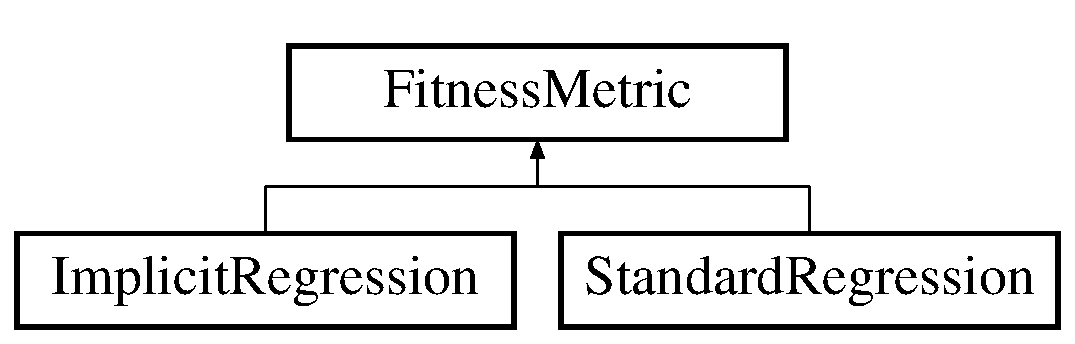
\includegraphics[height=2.000000cm]{structFitnessMetric}
\end{center}
\end{figure}
\subsection*{Public Member Functions}
\begin{DoxyCompactItemize}
\item 
virtual Eigen\+::\+Array\+X\+Xd \hyperlink{structFitnessMetric_a17bf921d3200dc93493e2af5c38552ad}{evaluate\+\_\+fitness\+\_\+vector} (\hyperlink{classAcyclicGraph}{Acyclic\+Graph} \&indv, \hyperlink{structTrainingData}{Training\+Data} \&train)=0
\begin{DoxyCompactList}\small\item\em f(x) -\/ y where f is defined by indv and x, y are in train \end{DoxyCompactList}\item 
double \hyperlink{structFitnessMetric_a8af896d7e25e1bf34412ce92b4851958}{evaluate\+\_\+fitness} (\hyperlink{classAcyclicGraph}{Acyclic\+Graph} \&indv, \hyperlink{structTrainingData}{Training\+Data} \&train)
\begin{DoxyCompactList}\small\item\em Finds the fitness metric. \end{DoxyCompactList}\item 
void \hyperlink{structFitnessMetric_ae4e27aefef6b54dddd6052bd80d37665}{optimize\+\_\+constants} (\hyperlink{classAcyclicGraph}{Acyclic\+Graph} \&indv, \hyperlink{structTrainingData}{Training\+Data} \&train)
\begin{DoxyCompactList}\small\item\em perform levenberg-\/marquardt optimization on embedded constants \end{DoxyCompactList}\end{DoxyCompactItemize}


\subsection{Detailed Description}
An abstract struct to evaluate metric based on type of regression

\begin{DoxyNote}{Note}
\hyperlink{structFitnessMetric}{Fitness\+Metric} includes \+: \hyperlink{structStandardRegression}{Standard\+Regression} 
\end{DoxyNote}


\subsection{Member Function Documentation}
\index{Fitness\+Metric@{Fitness\+Metric}!evaluate\+\_\+fitness@{evaluate\+\_\+fitness}}
\index{evaluate\+\_\+fitness@{evaluate\+\_\+fitness}!Fitness\+Metric@{Fitness\+Metric}}
\subsubsection[{\texorpdfstring{evaluate\+\_\+fitness(\+Acyclic\+Graph \&indv, Training\+Data \&train)}{evaluate_fitness(AcyclicGraph &indv, TrainingData &train)}}]{\setlength{\rightskip}{0pt plus 5cm}double Fitness\+Metric\+::evaluate\+\_\+fitness (
\begin{DoxyParamCaption}
\item[{{\bf Acyclic\+Graph} \&}]{indv, }
\item[{{\bf Training\+Data} \&}]{train}
\end{DoxyParamCaption}
)}\hypertarget{structFitnessMetric_a8af896d7e25e1bf34412ce92b4851958}{}\label{structFitnessMetric_a8af896d7e25e1bf34412ce92b4851958}


Finds the fitness metric. 


\begin{DoxyParams}[1]{Parameters}
\mbox{\tt in}  & {\em indv} & agcpp indv to be evaluated. \hyperlink{classAcyclicGraph}{Acyclic\+Graph} \\
\hline
\mbox{\tt in}  & {\em train} & The \hyperlink{structTrainingData}{Training\+Data} to evaluate the fitness. \hyperlink{structTrainingData}{Training\+Data} \\
\hline
\end{DoxyParams}
\begin{DoxyReturn}{Returns}
float the fitness metric 
\end{DoxyReturn}
\index{Fitness\+Metric@{Fitness\+Metric}!evaluate\+\_\+fitness\+\_\+vector@{evaluate\+\_\+fitness\+\_\+vector}}
\index{evaluate\+\_\+fitness\+\_\+vector@{evaluate\+\_\+fitness\+\_\+vector}!Fitness\+Metric@{Fitness\+Metric}}
\subsubsection[{\texorpdfstring{evaluate\+\_\+fitness\+\_\+vector(\+Acyclic\+Graph \&indv, Training\+Data \&train)=0}{evaluate_fitness_vector(AcyclicGraph &indv, TrainingData &train)=0}}]{\setlength{\rightskip}{0pt plus 5cm}virtual Eigen\+::\+Array\+X\+Xd Fitness\+Metric\+::evaluate\+\_\+fitness\+\_\+vector (
\begin{DoxyParamCaption}
\item[{{\bf Acyclic\+Graph} \&}]{indv, }
\item[{{\bf Training\+Data} \&}]{train}
\end{DoxyParamCaption}
)\hspace{0.3cm}{\ttfamily [pure virtual]}}\hypertarget{structFitnessMetric_a17bf921d3200dc93493e2af5c38552ad}{}\label{structFitnessMetric_a17bf921d3200dc93493e2af5c38552ad}


f(x) -\/ y where f is defined by indv and x, y are in train 

\begin{DoxyNote}{Note}
Each implementation will need to hard code casting \hyperlink{structTrainingData}{Training\+Data} to a specific type in this function.
\end{DoxyNote}

\begin{DoxyParams}[1]{Parameters}
\mbox{\tt in}  & {\em indv} & agcpp indv to be evaluated. \hyperlink{classAcyclicGraph}{Acyclic\+Graph} \\
\hline
\mbox{\tt in}  & {\em train} & The \hyperlink{structTrainingData}{Training\+Data} to evaluate the fitness. \hyperlink{structTrainingData}{Training\+Data} \\
\hline
\end{DoxyParams}
\begin{DoxyReturn}{Returns}
Eigen\+::\+Array\+X\+Xd the fitness vector 
\end{DoxyReturn}


Implemented in \hyperlink{structImplicitRegression_a8737c12d204ab5035347259f47018e5a}{Implicit\+Regression}, and \hyperlink{structStandardRegression_a0c35e5b8ce369988c8e1d6c3249b9581}{Standard\+Regression}.

\index{Fitness\+Metric@{Fitness\+Metric}!optimize\+\_\+constants@{optimize\+\_\+constants}}
\index{optimize\+\_\+constants@{optimize\+\_\+constants}!Fitness\+Metric@{Fitness\+Metric}}
\subsubsection[{\texorpdfstring{optimize\+\_\+constants(\+Acyclic\+Graph \&indv, Training\+Data \&train)}{optimize_constants(AcyclicGraph &indv, TrainingData &train)}}]{\setlength{\rightskip}{0pt plus 5cm}void Fitness\+Metric\+::optimize\+\_\+constants (
\begin{DoxyParamCaption}
\item[{{\bf Acyclic\+Graph} \&}]{indv, }
\item[{{\bf Training\+Data} \&}]{train}
\end{DoxyParamCaption}
)}\hypertarget{structFitnessMetric_ae4e27aefef6b54dddd6052bd80d37665}{}\label{structFitnessMetric_ae4e27aefef6b54dddd6052bd80d37665}


perform levenberg-\/marquardt optimization on embedded constants 


\begin{DoxyParams}[1]{Parameters}
\mbox{\tt in}  & {\em indv} & agcpp indv to be evaluated. \hyperlink{classAcyclicGraph}{Acyclic\+Graph} \\
\hline
\mbox{\tt in}  & {\em train} & The \hyperlink{structTrainingData}{Training\+Data} used by fitness metric. \hyperlink{structTrainingData}{Training\+Data} \\
\hline
\end{DoxyParams}


The documentation for this struct was generated from the following files\+:\begin{DoxyCompactItemize}
\item 
/users0/gbomarit/\+Projects/\+Genetic\+\_\+\+Programming/bingo/bingocpp/include/\+Bingo\+Cpp/\hyperlink{fitness__metric_8h}{fitness\+\_\+metric.\+h}\item 
/users0/gbomarit/\+Projects/\+Genetic\+\_\+\+Programming/bingo/bingocpp/src/fitness\+\_\+metric.\+cpp\end{DoxyCompactItemize}

\hypertarget{structImplicitRegression}{}\section{Implicit\+Regression Struct Reference}
\label{structImplicitRegression}\index{Implicit\+Regression@{Implicit\+Regression}}


Implicit Regression.  




{\ttfamily \#include $<$fitness\+\_\+metric.\+h$>$}

Inheritance diagram for Implicit\+Regression\+:\begin{figure}[H]
\begin{center}
\leavevmode
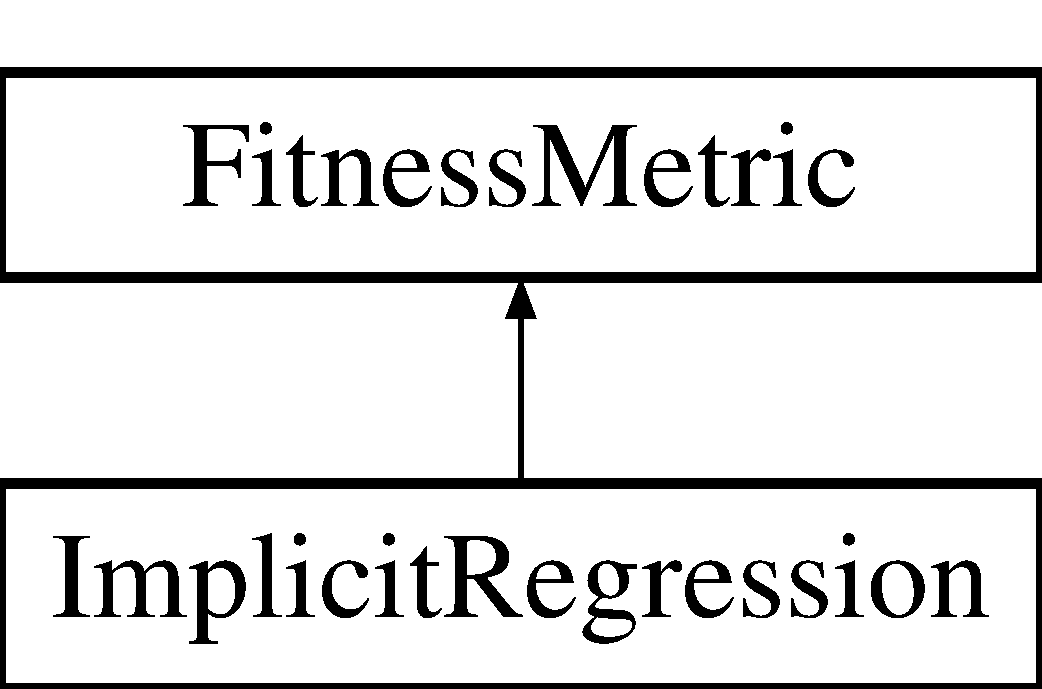
\includegraphics[height=2.000000cm]{structImplicitRegression}
\end{center}
\end{figure}
\subsection*{Public Member Functions}
\begin{DoxyCompactItemize}
\item 
{\bfseries Implicit\+Regression} (int \hyperlink{structImplicitRegression_a5f25461dae2b71ad79eaf7fb91c86696}{required\+\_\+params}=0, bool \hyperlink{structImplicitRegression_a8d31df5b4020c1d26dc130e694b69ee4}{normalize\+\_\+dot}=false, double acceptable\+\_\+nans=0.\+1)\hypertarget{structImplicitRegression_a5b70d19ebaa9e298a01a6eaf05b915f9}{}\label{structImplicitRegression_a5b70d19ebaa9e298a01a6eaf05b915f9}

\item 
Eigen\+::\+Array\+X\+Xd \hyperlink{structImplicitRegression_a8737c12d204ab5035347259f47018e5a}{evaluate\+\_\+fitness\+\_\+vector} (\hyperlink{classAcyclicGraph}{Acyclic\+Graph} \&indv, \hyperlink{structTrainingData}{Training\+Data} \&train)
\begin{DoxyCompactList}\small\item\em f(x) -\/ y where f is defined by indv and x, y are in train \end{DoxyCompactList}\end{DoxyCompactItemize}
\subsection*{Public Attributes}
\begin{DoxyCompactItemize}
\item 
int \hyperlink{structImplicitRegression_a5f25461dae2b71ad79eaf7fb91c86696}{required\+\_\+params}
\begin{DoxyCompactList}\small\item\em int required\+\_\+params \end{DoxyCompactList}\item 
bool \hyperlink{structImplicitRegression_a8d31df5b4020c1d26dc130e694b69ee4}{normalize\+\_\+dot}
\begin{DoxyCompactList}\small\item\em bool normalize\+\_\+dot \end{DoxyCompactList}\item 
double \hyperlink{structImplicitRegression_ae74f24de0d7a6a9fb3cab6e6a8b9e560}{acceptable\+\_\+finite\+\_\+fracion}
\begin{DoxyCompactList}\small\item\em double acceptable\+\_\+finite\+\_\+fracion \end{DoxyCompactList}\end{DoxyCompactItemize}


\subsection{Detailed Description}
Implicit Regression. 

\subsection{Member Function Documentation}
\index{Implicit\+Regression@{Implicit\+Regression}!evaluate\+\_\+fitness\+\_\+vector@{evaluate\+\_\+fitness\+\_\+vector}}
\index{evaluate\+\_\+fitness\+\_\+vector@{evaluate\+\_\+fitness\+\_\+vector}!Implicit\+Regression@{Implicit\+Regression}}
\subsubsection[{\texorpdfstring{evaluate\+\_\+fitness\+\_\+vector(\+Acyclic\+Graph \&indv, Training\+Data \&train)}{evaluate_fitness_vector(AcyclicGraph &indv, TrainingData &train)}}]{\setlength{\rightskip}{0pt plus 5cm}Eigen\+::\+Array\+X\+Xd Implicit\+Regression\+::evaluate\+\_\+fitness\+\_\+vector (
\begin{DoxyParamCaption}
\item[{{\bf Acyclic\+Graph} \&}]{indv, }
\item[{{\bf Training\+Data} \&}]{train}
\end{DoxyParamCaption}
)\hspace{0.3cm}{\ttfamily [virtual]}}\hypertarget{structImplicitRegression_a8737c12d204ab5035347259f47018e5a}{}\label{structImplicitRegression_a8737c12d204ab5035347259f47018e5a}


f(x) -\/ y where f is defined by indv and x, y are in train 

\begin{DoxyNote}{Note}
Each implementation will need to hard code casting \hyperlink{structTrainingData}{Training\+Data} to a specific type in this function.
\end{DoxyNote}

\begin{DoxyParams}[1]{Parameters}
\mbox{\tt in}  & {\em indv} & agcpp indv to be evaluated. \hyperlink{classAcyclicGraph}{Acyclic\+Graph} \\
\hline
\mbox{\tt in}  & {\em train} & The \hyperlink{structTrainingData}{Training\+Data} to evaluate the fitness. \hyperlink{structTrainingData}{Training\+Data} \\
\hline
\end{DoxyParams}
\begin{DoxyReturn}{Returns}
Eigen\+::\+Array\+X\+Xd the fitness vector 
\end{DoxyReturn}


Implements \hyperlink{structFitnessMetric_a17bf921d3200dc93493e2af5c38552ad}{Fitness\+Metric}.



\subsection{Member Data Documentation}
\index{Implicit\+Regression@{Implicit\+Regression}!acceptable\+\_\+finite\+\_\+fracion@{acceptable\+\_\+finite\+\_\+fracion}}
\index{acceptable\+\_\+finite\+\_\+fracion@{acceptable\+\_\+finite\+\_\+fracion}!Implicit\+Regression@{Implicit\+Regression}}
\subsubsection[{\texorpdfstring{acceptable\+\_\+finite\+\_\+fracion}{acceptable_finite_fracion}}]{\setlength{\rightskip}{0pt plus 5cm}double Implicit\+Regression\+::acceptable\+\_\+finite\+\_\+fracion}\hypertarget{structImplicitRegression_ae74f24de0d7a6a9fb3cab6e6a8b9e560}{}\label{structImplicitRegression_ae74f24de0d7a6a9fb3cab6e6a8b9e560}


double acceptable\+\_\+finite\+\_\+fracion 

yea \index{Implicit\+Regression@{Implicit\+Regression}!normalize\+\_\+dot@{normalize\+\_\+dot}}
\index{normalize\+\_\+dot@{normalize\+\_\+dot}!Implicit\+Regression@{Implicit\+Regression}}
\subsubsection[{\texorpdfstring{normalize\+\_\+dot}{normalize_dot}}]{\setlength{\rightskip}{0pt plus 5cm}bool Implicit\+Regression\+::normalize\+\_\+dot}\hypertarget{structImplicitRegression_a8d31df5b4020c1d26dc130e694b69ee4}{}\label{structImplicitRegression_a8d31df5b4020c1d26dc130e694b69ee4}


bool normalize\+\_\+dot 

normalize the terms in the dot product \index{Implicit\+Regression@{Implicit\+Regression}!required\+\_\+params@{required\+\_\+params}}
\index{required\+\_\+params@{required\+\_\+params}!Implicit\+Regression@{Implicit\+Regression}}
\subsubsection[{\texorpdfstring{required\+\_\+params}{required_params}}]{\setlength{\rightskip}{0pt plus 5cm}int Implicit\+Regression\+::required\+\_\+params}\hypertarget{structImplicitRegression_a5f25461dae2b71ad79eaf7fb91c86696}{}\label{structImplicitRegression_a5f25461dae2b71ad79eaf7fb91c86696}


int required\+\_\+params 

minimum number of non zero components of dot 

The documentation for this struct was generated from the following files\+:\begin{DoxyCompactItemize}
\item 
/users0/gbomarit/\+Projects/\+Genetic\+\_\+\+Programming/bingo/bingocpp/include/\+Bingo\+Cpp/\hyperlink{fitness__metric_8h}{fitness\+\_\+metric.\+h}\item 
/users0/gbomarit/\+Projects/\+Genetic\+\_\+\+Programming/bingo/bingocpp/src/fitness\+\_\+metric.\+cpp\end{DoxyCompactItemize}

\hypertarget{structImplicitTrainingData}{}\section{Implicit\+Training\+Data Struct Reference}
\label{structImplicitTrainingData}\index{Implicit\+Training\+Data@{Implicit\+Training\+Data}}


This struct holds data for Implicit regression.  




{\ttfamily \#include $<$training\+\_\+data.\+h$>$}

Inheritance diagram for Implicit\+Training\+Data\+:\begin{figure}[H]
\begin{center}
\leavevmode
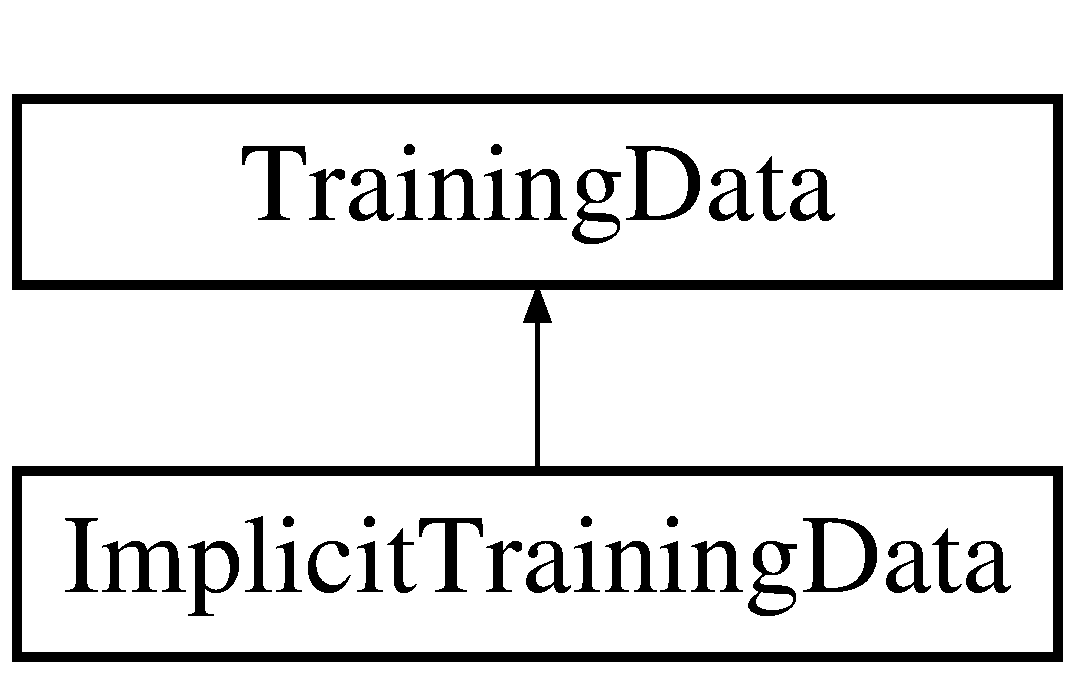
\includegraphics[height=2.000000cm]{structImplicitTrainingData}
\end{center}
\end{figure}
\subsection*{Public Member Functions}
\begin{DoxyCompactItemize}
\item 
\hyperlink{structImplicitTrainingData_a517aa36137750f3d4299491b030b7431}{Implicit\+Training\+Data} (Eigen\+::\+Array\+X\+Xd vx)\hypertarget{structImplicitTrainingData_a517aa36137750f3d4299491b030b7431}{}\label{structImplicitTrainingData_a517aa36137750f3d4299491b030b7431}

\begin{DoxyCompactList}\small\item\em Constructor. \end{DoxyCompactList}\item 
\hyperlink{structImplicitTrainingData_a5bea19d7ebed073cab7dbad3a0aeaeb2}{Implicit\+Training\+Data} (Eigen\+::\+Array\+X\+Xd vx, Eigen\+::\+Array\+X\+Xd vdx\+\_\+dt)\hypertarget{structImplicitTrainingData_a5bea19d7ebed073cab7dbad3a0aeaeb2}{}\label{structImplicitTrainingData_a5bea19d7ebed073cab7dbad3a0aeaeb2}

\begin{DoxyCompactList}\small\item\em Constructor. \end{DoxyCompactList}\item 
\hyperlink{structImplicitTrainingData}{Implicit\+Training\+Data} $\ast$ \hyperlink{structImplicitTrainingData_a91e92604cc19a693ac89eb7dbd9fab80}{get\+\_\+item} (std\+::list$<$ int $>$ items)
\begin{DoxyCompactList}\small\item\em gets a new training data with certain rows \end{DoxyCompactList}\item 
int \hyperlink{structImplicitTrainingData_aa3be8b04a160fb496668bba52507d3e4}{size} ()
\begin{DoxyCompactList}\small\item\em gets the size of x \end{DoxyCompactList}\end{DoxyCompactItemize}
\subsection*{Public Attributes}
\begin{DoxyCompactItemize}
\item 
Eigen\+::\+Array\+X\+Xd \hyperlink{structImplicitTrainingData_a7d797c666ce6c25d2f816e01ed4f3aed}{x}
\begin{DoxyCompactList}\small\item\em Eigen\+::\+Array\+X\+Xd x. \end{DoxyCompactList}\item 
Eigen\+::\+Array\+X\+Xd \hyperlink{structImplicitTrainingData_a46e7205b1b43da1e0b6b582b3d127a2e}{dx\+\_\+dt}
\begin{DoxyCompactList}\small\item\em Eigen\+::\+Array\+X\+Xd dx\+\_\+dt. \end{DoxyCompactList}\end{DoxyCompactItemize}


\subsection{Detailed Description}
This struct holds data for Implicit regression. 

\subsection{Member Function Documentation}
\index{Implicit\+Training\+Data@{Implicit\+Training\+Data}!get\+\_\+item@{get\+\_\+item}}
\index{get\+\_\+item@{get\+\_\+item}!Implicit\+Training\+Data@{Implicit\+Training\+Data}}
\subsubsection[{\texorpdfstring{get\+\_\+item(std\+::list$<$ int $>$ items)}{get_item(std::list< int > items)}}]{\setlength{\rightskip}{0pt plus 5cm}{\bf Implicit\+Training\+Data} $\ast$ Implicit\+Training\+Data\+::get\+\_\+item (
\begin{DoxyParamCaption}
\item[{std\+::list$<$ int $>$}]{items}
\end{DoxyParamCaption}
)\hspace{0.3cm}{\ttfamily [virtual]}}\hypertarget{structImplicitTrainingData_a91e92604cc19a693ac89eb7dbd9fab80}{}\label{structImplicitTrainingData_a91e92604cc19a693ac89eb7dbd9fab80}


gets a new training data with certain rows 


\begin{DoxyParams}[1]{Parameters}
\mbox{\tt in}  & {\em items} & The rows to retrieve. std\+::list$<$int$>$ \\
\hline
\end{DoxyParams}
\begin{DoxyReturn}{Returns}
Training\+Data$\ast$ with the selected data 
\end{DoxyReturn}


Implements \hyperlink{structTrainingData_a96ef790e9e78909f84ce83692c7faced}{Training\+Data}.

\index{Implicit\+Training\+Data@{Implicit\+Training\+Data}!size@{size}}
\index{size@{size}!Implicit\+Training\+Data@{Implicit\+Training\+Data}}
\subsubsection[{\texorpdfstring{size()}{size()}}]{\setlength{\rightskip}{0pt plus 5cm}int Implicit\+Training\+Data\+::size (
\begin{DoxyParamCaption}
{}
\end{DoxyParamCaption}
)\hspace{0.3cm}{\ttfamily [inline]}, {\ttfamily [virtual]}}\hypertarget{structImplicitTrainingData_aa3be8b04a160fb496668bba52507d3e4}{}\label{structImplicitTrainingData_aa3be8b04a160fb496668bba52507d3e4}


gets the size of x 

\begin{DoxyReturn}{Returns}
int the amount of rows in x 
\end{DoxyReturn}


Implements \hyperlink{structTrainingData_a9be21e878961cc347e6820eb34db0a1b}{Training\+Data}.



\subsection{Member Data Documentation}
\index{Implicit\+Training\+Data@{Implicit\+Training\+Data}!dx\+\_\+dt@{dx\+\_\+dt}}
\index{dx\+\_\+dt@{dx\+\_\+dt}!Implicit\+Training\+Data@{Implicit\+Training\+Data}}
\subsubsection[{\texorpdfstring{dx\+\_\+dt}{dx_dt}}]{\setlength{\rightskip}{0pt plus 5cm}Eigen\+::\+Array\+X\+Xd Implicit\+Training\+Data\+::dx\+\_\+dt}\hypertarget{structImplicitTrainingData_a46e7205b1b43da1e0b6b582b3d127a2e}{}\label{structImplicitTrainingData_a46e7205b1b43da1e0b6b582b3d127a2e}


Eigen\+::\+Array\+X\+Xd dx\+\_\+dt. 

dx\+\_\+dt variabes for Implicit\+Training \index{Implicit\+Training\+Data@{Implicit\+Training\+Data}!x@{x}}
\index{x@{x}!Implicit\+Training\+Data@{Implicit\+Training\+Data}}
\subsubsection[{\texorpdfstring{x}{x}}]{\setlength{\rightskip}{0pt plus 5cm}Eigen\+::\+Array\+X\+Xd Implicit\+Training\+Data\+::x}\hypertarget{structImplicitTrainingData_a7d797c666ce6c25d2f816e01ed4f3aed}{}\label{structImplicitTrainingData_a7d797c666ce6c25d2f816e01ed4f3aed}


Eigen\+::\+Array\+X\+Xd x. 

x variabes for Implicit\+Training 

The documentation for this struct was generated from the following files\+:\begin{DoxyCompactItemize}
\item 
/users0/gbomarit/\+Projects/\+Genetic\+\_\+\+Programming/bingo/bingocpp/include/\+Bingo\+Cpp/\hyperlink{training__data_8h}{training\+\_\+data.\+h}\item 
/users0/gbomarit/\+Projects/\+Genetic\+\_\+\+Programming/bingo/bingocpp/src/training\+\_\+data.\+cpp\end{DoxyCompactItemize}

\hypertarget{structLMFunctor}{}\section{L\+M\+Functor Struct Reference}
\label{structLMFunctor}\index{L\+M\+Functor@{L\+M\+Functor}}


{\ttfamily \#include $<$fitness\+\_\+metric.\+h$>$}

\subsection*{Public Member Functions}
\begin{DoxyCompactItemize}
\item 
int \hyperlink{structLMFunctor_ab9272cf916bc55507969dff595743dfe}{operator()} (const Eigen\+::\+Vector\+Xd \&x, Eigen\+::\+Vector\+Xd \&fvec)
\begin{DoxyCompactList}\small\item\em Compute \textquotesingle{}m\textquotesingle{} errors, one for each data point, for the given paramter values in \textquotesingle{}x\textquotesingle{}. \end{DoxyCompactList}\item 
int \hyperlink{structLMFunctor_a0f2edfe1662d360c601caec4332ab60a}{df} (const Eigen\+::\+Vector\+Xd \&x, Eigen\+::\+Matrix\+Xd \&fjac)
\begin{DoxyCompactList}\small\item\em Compute jacobian of the errors. \end{DoxyCompactList}\item 
int \hyperlink{structLMFunctor_a928ebbc0ae61ab4fe5e9ffa0111f38e7}{values} () const 
\begin{DoxyCompactList}\small\item\em gets the values \end{DoxyCompactList}\item 
int \hyperlink{structLMFunctor_af3216685479be9d9c3d7fc5066927d02}{inputs} () const 
\begin{DoxyCompactList}\small\item\em gets the inputs \end{DoxyCompactList}\end{DoxyCompactItemize}
\subsection*{Public Attributes}
\begin{DoxyCompactItemize}
\item 
int \hyperlink{structLMFunctor_a090d075bceebea8c93aa70a99e7620d5}{m}
\begin{DoxyCompactList}\small\item\em int m \end{DoxyCompactList}\item 
int \hyperlink{structLMFunctor_a97d53b5fcdf96c8ffe5ea70b7adc0de4}{n}
\begin{DoxyCompactList}\small\item\em int n \end{DoxyCompactList}\item 
\hyperlink{classAcyclicGraph}{Acyclic\+Graph} \hyperlink{structLMFunctor_aece2cab33ffd2f919fe9e6817e3a85ac}{agraph\+Indv}
\begin{DoxyCompactList}\small\item\em \hyperlink{classAcyclicGraph}{Acyclic\+Graph} indv. \end{DoxyCompactList}\item 
\hyperlink{structTrainingData}{Training\+Data} $\ast$ \hyperlink{structLMFunctor_a025c08d9282710fb0766dcee6dd8ff07}{train}
\begin{DoxyCompactList}\small\item\em Training\+Data$\ast$ train. \end{DoxyCompactList}\item 
\hyperlink{structFitnessMetric}{Fitness\+Metric} $\ast$ \hyperlink{structLMFunctor_a39d6ef99670d28134bd7a903993f5e23}{fit}
\begin{DoxyCompactList}\small\item\em Fitness\+Metric$\ast$ fit. \end{DoxyCompactList}\end{DoxyCompactItemize}


\subsection{Detailed Description}
Used for Levenberg-\/\+Marquardt Optimization 

\subsection{Member Function Documentation}
\index{L\+M\+Functor@{L\+M\+Functor}!df@{df}}
\index{df@{df}!L\+M\+Functor@{L\+M\+Functor}}
\subsubsection[{\texorpdfstring{df(const Eigen\+::\+Vector\+Xd \&x, Eigen\+::\+Matrix\+Xd \&fjac)}{df(const Eigen::VectorXd &x, Eigen::MatrixXd &fjac)}}]{\setlength{\rightskip}{0pt plus 5cm}int L\+M\+Functor\+::df (
\begin{DoxyParamCaption}
\item[{const Eigen\+::\+Vector\+Xd \&}]{x, }
\item[{Eigen\+::\+Matrix\+Xd \&}]{fjac}
\end{DoxyParamCaption}
)}\hypertarget{structLMFunctor_a0f2edfe1662d360c601caec4332ab60a}{}\label{structLMFunctor_a0f2edfe1662d360c601caec4332ab60a}


Compute jacobian of the errors. 


\begin{DoxyParams}[1]{Parameters}
\mbox{\tt in}  & {\em x} & contains current estimates for parameters. Eigen\+::\+Vector\+Xd (dimensions nx1) \\
\hline
\mbox{\tt in}  & {\em fjac} & contain jacobian of the errors, calculated numerically. Eigen\+::\+Matrix\+Xf (dimensions mxn) \\
\hline
\end{DoxyParams}
\begin{DoxyReturn}{Returns}
0 
\end{DoxyReturn}
\index{L\+M\+Functor@{L\+M\+Functor}!inputs@{inputs}}
\index{inputs@{inputs}!L\+M\+Functor@{L\+M\+Functor}}
\subsubsection[{\texorpdfstring{inputs() const }{inputs() const }}]{\setlength{\rightskip}{0pt plus 5cm}int L\+M\+Functor\+::inputs (
\begin{DoxyParamCaption}
{}
\end{DoxyParamCaption}
) const\hspace{0.3cm}{\ttfamily [inline]}}\hypertarget{structLMFunctor_af3216685479be9d9c3d7fc5066927d02}{}\label{structLMFunctor_af3216685479be9d9c3d7fc5066927d02}


gets the inputs 

\begin{DoxyReturn}{Returns}
n -\/ inputs 
\end{DoxyReturn}
\index{L\+M\+Functor@{L\+M\+Functor}!operator()@{operator()}}
\index{operator()@{operator()}!L\+M\+Functor@{L\+M\+Functor}}
\subsubsection[{\texorpdfstring{operator()(const Eigen\+::\+Vector\+Xd \&x, Eigen\+::\+Vector\+Xd \&fvec)}{operator()(const Eigen::VectorXd &x, Eigen::VectorXd &fvec)}}]{\setlength{\rightskip}{0pt plus 5cm}int L\+M\+Functor\+::operator() (
\begin{DoxyParamCaption}
\item[{const Eigen\+::\+Vector\+Xd \&}]{x, }
\item[{Eigen\+::\+Vector\+Xd \&}]{fvec}
\end{DoxyParamCaption}
)}\hypertarget{structLMFunctor_ab9272cf916bc55507969dff595743dfe}{}\label{structLMFunctor_ab9272cf916bc55507969dff595743dfe}


Compute \textquotesingle{}m\textquotesingle{} errors, one for each data point, for the given paramter values in \textquotesingle{}x\textquotesingle{}. 


\begin{DoxyParams}[1]{Parameters}
\mbox{\tt in}  & {\em x} & contains current estimates for parameters. Eigen\+::\+Vector\+Xd (dimensions nx1) \\
\hline
\mbox{\tt in}  & {\em fvec} & contain error for each data point. Eigen\+::\+Vector\+Xd (dimensions mx1) \\
\hline
\end{DoxyParams}
\begin{DoxyReturn}{Returns}
0 
\end{DoxyReturn}
\index{L\+M\+Functor@{L\+M\+Functor}!values@{values}}
\index{values@{values}!L\+M\+Functor@{L\+M\+Functor}}
\subsubsection[{\texorpdfstring{values() const }{values() const }}]{\setlength{\rightskip}{0pt plus 5cm}int L\+M\+Functor\+::values (
\begin{DoxyParamCaption}
{}
\end{DoxyParamCaption}
) const\hspace{0.3cm}{\ttfamily [inline]}}\hypertarget{structLMFunctor_a928ebbc0ae61ab4fe5e9ffa0111f38e7}{}\label{structLMFunctor_a928ebbc0ae61ab4fe5e9ffa0111f38e7}


gets the values 

\begin{DoxyReturn}{Returns}
m -\/ values 
\end{DoxyReturn}


\subsection{Member Data Documentation}
\index{L\+M\+Functor@{L\+M\+Functor}!agraph\+Indv@{agraph\+Indv}}
\index{agraph\+Indv@{agraph\+Indv}!L\+M\+Functor@{L\+M\+Functor}}
\subsubsection[{\texorpdfstring{agraph\+Indv}{agraphIndv}}]{\setlength{\rightskip}{0pt plus 5cm}{\bf Acyclic\+Graph} L\+M\+Functor\+::agraph\+Indv}\hypertarget{structLMFunctor_aece2cab33ffd2f919fe9e6817e3a85ac}{}\label{structLMFunctor_aece2cab33ffd2f919fe9e6817e3a85ac}


\hyperlink{classAcyclicGraph}{Acyclic\+Graph} indv. 

The Agraph individual \index{L\+M\+Functor@{L\+M\+Functor}!fit@{fit}}
\index{fit@{fit}!L\+M\+Functor@{L\+M\+Functor}}
\subsubsection[{\texorpdfstring{fit}{fit}}]{\setlength{\rightskip}{0pt plus 5cm}{\bf Fitness\+Metric}$\ast$ L\+M\+Functor\+::fit}\hypertarget{structLMFunctor_a39d6ef99670d28134bd7a903993f5e23}{}\label{structLMFunctor_a39d6ef99670d28134bd7a903993f5e23}


Fitness\+Metric$\ast$ fit. 

object that holds fitness metric \index{L\+M\+Functor@{L\+M\+Functor}!m@{m}}
\index{m@{m}!L\+M\+Functor@{L\+M\+Functor}}
\subsubsection[{\texorpdfstring{m}{m}}]{\setlength{\rightskip}{0pt plus 5cm}int L\+M\+Functor\+::m}\hypertarget{structLMFunctor_a090d075bceebea8c93aa70a99e7620d5}{}\label{structLMFunctor_a090d075bceebea8c93aa70a99e7620d5}


int m 

Number of data points, i.\+e. values \index{L\+M\+Functor@{L\+M\+Functor}!n@{n}}
\index{n@{n}!L\+M\+Functor@{L\+M\+Functor}}
\subsubsection[{\texorpdfstring{n}{n}}]{\setlength{\rightskip}{0pt plus 5cm}int L\+M\+Functor\+::n}\hypertarget{structLMFunctor_a97d53b5fcdf96c8ffe5ea70b7adc0de4}{}\label{structLMFunctor_a97d53b5fcdf96c8ffe5ea70b7adc0de4}


int n 

Number of parameters, i.\+e. inputs \index{L\+M\+Functor@{L\+M\+Functor}!train@{train}}
\index{train@{train}!L\+M\+Functor@{L\+M\+Functor}}
\subsubsection[{\texorpdfstring{train}{train}}]{\setlength{\rightskip}{0pt plus 5cm}{\bf Training\+Data}$\ast$ L\+M\+Functor\+::train}\hypertarget{structLMFunctor_a025c08d9282710fb0766dcee6dd8ff07}{}\label{structLMFunctor_a025c08d9282710fb0766dcee6dd8ff07}


Training\+Data$\ast$ train. 

object that holds data needed 

The documentation for this struct was generated from the following files\+:\begin{DoxyCompactItemize}
\item 
/users0/gbomarit/\+Projects/\+Genetic\+\_\+\+Programming/bingo/bingocpp/include/\+Bingo\+Cpp/\hyperlink{fitness__metric_8h}{fitness\+\_\+metric.\+h}\item 
/users0/gbomarit/\+Projects/\+Genetic\+\_\+\+Programming/bingo/bingocpp/src/fitness\+\_\+metric.\+cpp\end{DoxyCompactItemize}

\hypertarget{classLog}{}\section{Log Class Reference}
\label{classLog}\index{Log@{Log}}


This class performs a safe log.  




{\ttfamily \#include $<$acyclic\+\_\+graph\+\_\+nodes.\+h$>$}

Inheritance diagram for Log\+:\begin{figure}[H]
\begin{center}
\leavevmode
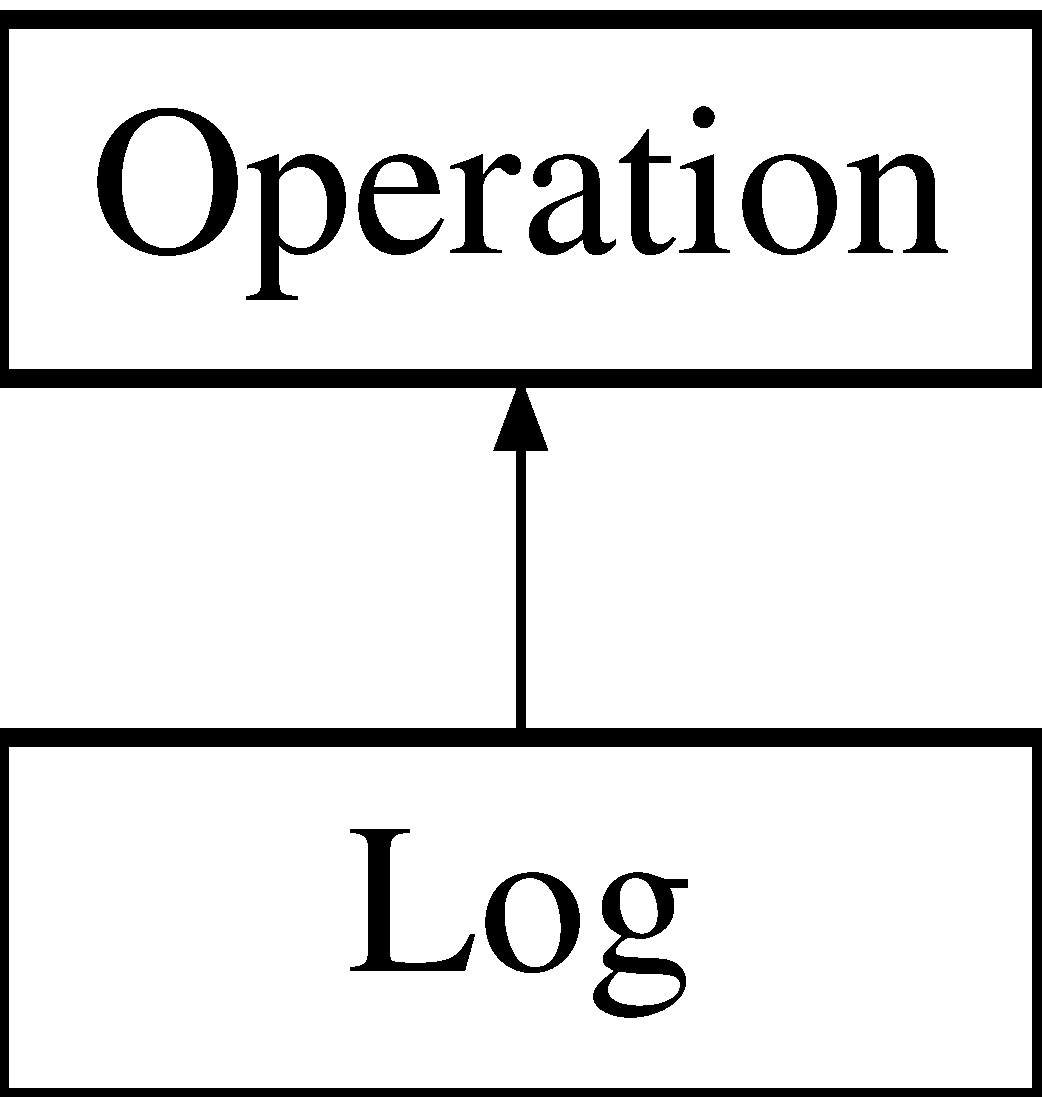
\includegraphics[height=2.000000cm]{classLog}
\end{center}
\end{figure}
\subsection*{Public Member Functions}
\begin{DoxyCompactItemize}
\item 
int \hyperlink{classLog_a42d5513e8506369af7372aaba01c58b3}{get\+\_\+arity} ()\hypertarget{classLog_a42d5513e8506369af7372aaba01c58b3}{}\label{classLog_a42d5513e8506369af7372aaba01c58b3}

\begin{DoxyCompactList}\small\item\em Returns how many parameters the operation requires. \end{DoxyCompactList}\item 
std\+::string \hyperlink{classLog_a218147ad7dbad6c9385810b5c79453b9}{get\+\_\+print} ()\hypertarget{classLog_a218147ad7dbad6c9385810b5c79453b9}{}\label{classLog_a218147ad7dbad6c9385810b5c79453b9}

\begin{DoxyCompactList}\small\item\em Returns the string representation of the operator. \end{DoxyCompactList}\item 
virtual void \hyperlink{classLog_af5402c400512ee9dfe17698929683bbc}{evaluate} (const Eigen\+::\+Array\+X3i \&stack, const Eigen\+::\+Array\+X\+Xd \&x, const Eigen\+::\+Vector\+Xd \&constants, std\+::vector$<$ Eigen\+::\+Array\+X\+Xd $>$ \&buffer, std\+::size\+\_\+t result\+\_\+location)
\begin{DoxyCompactList}\small\item\em evaluates a single command at the location passed in \end{DoxyCompactList}\item 
virtual void \hyperlink{classLog_a6f52d16f62171275092117364faa9b04}{deriv\+\_\+evaluate} (const Eigen\+::\+Array\+X3i \&stack, const int command\+\_\+index, const std\+::vector$<$ Eigen\+::\+Array\+X\+Xd $>$ \&forward\+\_\+buffer, std\+::vector$<$ Eigen\+::\+Array\+X\+Xd $>$ \&reverse\+\_\+buffer, int dependency)
\begin{DoxyCompactList}\small\item\em Computes reverse autodiff partial of a command stack. \end{DoxyCompactList}\end{DoxyCompactItemize}


\subsection{Detailed Description}
This class performs a safe log. 

\subsection{Member Function Documentation}
\index{Log@{Log}!deriv\+\_\+evaluate@{deriv\+\_\+evaluate}}
\index{deriv\+\_\+evaluate@{deriv\+\_\+evaluate}!Log@{Log}}
\subsubsection[{\texorpdfstring{deriv\+\_\+evaluate(const Eigen\+::\+Array\+X3i \&stack, const int command\+\_\+index, const std\+::vector$<$ Eigen\+::\+Array\+X\+Xd $>$ \&forward\+\_\+buffer, std\+::vector$<$ Eigen\+::\+Array\+X\+Xd $>$ \&reverse\+\_\+buffer, int dependency)}{deriv_evaluate(const Eigen::ArrayX3i &stack, const int command_index, const std::vector< Eigen::ArrayXXd > &forward_buffer, std::vector< Eigen::ArrayXXd > &reverse_buffer, int dependency)}}]{\setlength{\rightskip}{0pt plus 5cm}void Log\+::deriv\+\_\+evaluate (
\begin{DoxyParamCaption}
\item[{const Eigen\+::\+Array\+X3i \&}]{stack, }
\item[{const int}]{command\+\_\+index, }
\item[{const std\+::vector$<$ Eigen\+::\+Array\+X\+Xd $>$ \&}]{forward\+\_\+buffer, }
\item[{std\+::vector$<$ Eigen\+::\+Array\+X\+Xd $>$ \&}]{reverse\+\_\+buffer, }
\item[{int}]{dependency}
\end{DoxyParamCaption}
)\hspace{0.3cm}{\ttfamily [virtual]}}\hypertarget{classLog_a6f52d16f62171275092117364faa9b04}{}\label{classLog_a6f52d16f62171275092117364faa9b04}


Computes reverse autodiff partial of a command stack. 


\begin{DoxyParams}[1]{Parameters}
\mbox{\tt in}  & {\em stack} & The stack that contains each command. Eigen\+::\+Array\+X3i \\
\hline
\mbox{\tt in}  & {\em command\+\_\+index} & Index of command in the command; also the location of the result to be placed in the reverse buffer. \\
\hline
\mbox{\tt in}  & {\em forward\+\_\+buffer} & Vector of Eigen arrays for the forward buffer. \\
\hline
 & {\em } & \\
\hline
\end{DoxyParams}


Implements \hyperlink{classOperation_a42b611d08c6b00568c5d1b08688ebcce}{Operation}.

\index{Log@{Log}!evaluate@{evaluate}}
\index{evaluate@{evaluate}!Log@{Log}}
\subsubsection[{\texorpdfstring{evaluate(const Eigen\+::\+Array\+X3i \&stack, const Eigen\+::\+Array\+X\+Xd \&x, const Eigen\+::\+Vector\+Xd \&constants, std\+::vector$<$ Eigen\+::\+Array\+X\+Xd $>$ \&buffer, std\+::size\+\_\+t result\+\_\+location)}{evaluate(const Eigen::ArrayX3i &stack, const Eigen::ArrayXXd &x, const Eigen::VectorXd &constants, std::vector< Eigen::ArrayXXd > &buffer, std::size_t result_location)}}]{\setlength{\rightskip}{0pt plus 5cm}void Log\+::evaluate (
\begin{DoxyParamCaption}
\item[{const Eigen\+::\+Array\+X3i \&}]{stack, }
\item[{const Eigen\+::\+Array\+X\+Xd \&}]{x, }
\item[{const Eigen\+::\+Vector\+Xd \&}]{constants, }
\item[{std\+::vector$<$ Eigen\+::\+Array\+X\+Xd $>$ \&}]{buffer, }
\item[{std\+::size\+\_\+t}]{result\+\_\+location}
\end{DoxyParamCaption}
)\hspace{0.3cm}{\ttfamily [virtual]}}\hypertarget{classLog_af5402c400512ee9dfe17698929683bbc}{}\label{classLog_af5402c400512ee9dfe17698929683bbc}


evaluates a single command at the location passed in 


\begin{DoxyParams}[1]{Parameters}
\mbox{\tt in}  & {\em stack} & The stack that contains each command. Eigen\+::\+Array\+X3i \\
\hline
\mbox{\tt in}  & {\em x} & Input variables to the acyclic graph. Eigen\+::\+Array\+X\+Xd \\
\hline
\mbox{\tt in}  & {\em constants} & Constants used in the command. Eigen\+::\+Vector\+Xd \\
\hline
 & {\em } & \\
\hline
\end{DoxyParams}


Implements \hyperlink{classOperation_a89093eb53f975dd98b6a36d85fa17276}{Operation}.



The documentation for this class was generated from the following files\+:\begin{DoxyCompactItemize}
\item 
/users0/gbomarit/\+Projects/\+Genetic\+\_\+\+Programming/bingo/bingocpp/include/\+Bingo\+Cpp/acyclic\+\_\+graph\+\_\+nodes.\+h\item 
/users0/gbomarit/\+Projects/\+Genetic\+\_\+\+Programming/bingo/bingocpp/src/acyclic\+\_\+graph\+\_\+nodes.\+cpp\end{DoxyCompactItemize}

\hypertarget{classMultiplication}{}\section{Multiplication Class Reference}
\label{classMultiplication}\index{Multiplication@{Multiplication}}


This class performs multiplication.  




{\ttfamily \#include $<$acyclic\+\_\+graph\+\_\+nodes.\+h$>$}

Inheritance diagram for Multiplication\+:\begin{figure}[H]
\begin{center}
\leavevmode
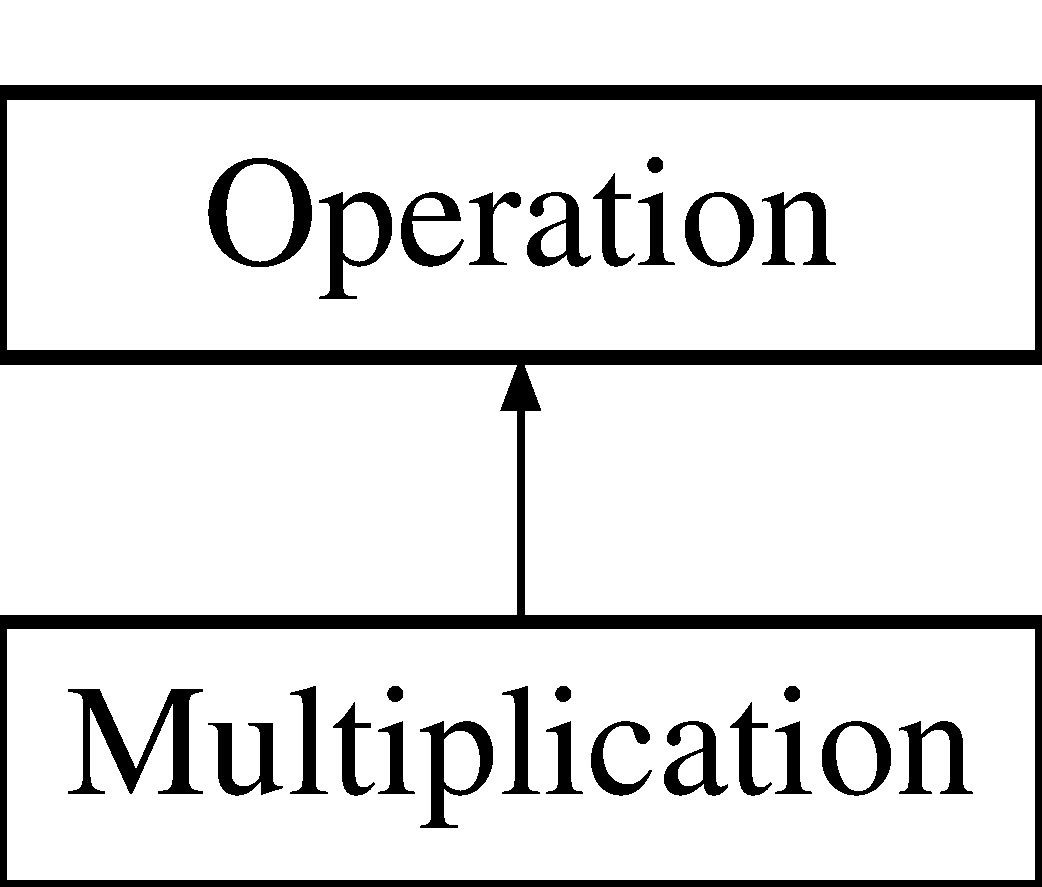
\includegraphics[height=2.000000cm]{classMultiplication}
\end{center}
\end{figure}
\subsection*{Public Member Functions}
\begin{DoxyCompactItemize}
\item 
int \hyperlink{classMultiplication_a696c850947f8fb31ad471dde80e8d2d2}{get\+\_\+arity} ()\hypertarget{classMultiplication_a696c850947f8fb31ad471dde80e8d2d2}{}\label{classMultiplication_a696c850947f8fb31ad471dde80e8d2d2}

\begin{DoxyCompactList}\small\item\em Returns how many parameters the operation requires. \end{DoxyCompactList}\item 
std\+::string \hyperlink{classMultiplication_aaa0b55c91c439c1d471fa5357b6b83a8}{get\+\_\+print} ()\hypertarget{classMultiplication_aaa0b55c91c439c1d471fa5357b6b83a8}{}\label{classMultiplication_aaa0b55c91c439c1d471fa5357b6b83a8}

\begin{DoxyCompactList}\small\item\em Returns the string representation of the operator. \end{DoxyCompactList}\item 
virtual void \hyperlink{classMultiplication_a19044777a8cc6ba3bc662d1fbadb7b28}{evaluate} (const Eigen\+::\+Array\+X3i \&stack, const Eigen\+::\+Array\+X\+Xd \&x, const Eigen\+::\+Vector\+Xd \&constants, std\+::vector$<$ Eigen\+::\+Array\+X\+Xd $>$ \&buffer, std\+::size\+\_\+t result\+\_\+location)
\begin{DoxyCompactList}\small\item\em evaluates a single command at the location passed in \end{DoxyCompactList}\item 
virtual void \hyperlink{classMultiplication_add5b53fbcd0f2e16c3be398c53d0fbe6}{deriv\+\_\+evaluate} (const Eigen\+::\+Array\+X3i \&stack, const int command\+\_\+index, const std\+::vector$<$ Eigen\+::\+Array\+X\+Xd $>$ \&forward\+\_\+buffer, std\+::vector$<$ Eigen\+::\+Array\+X\+Xd $>$ \&reverse\+\_\+buffer, int dependency)
\begin{DoxyCompactList}\small\item\em Computes reverse autodiff partial of a command stack. \end{DoxyCompactList}\end{DoxyCompactItemize}


\subsection{Detailed Description}
This class performs multiplication. 

\subsection{Member Function Documentation}
\index{Multiplication@{Multiplication}!deriv\+\_\+evaluate@{deriv\+\_\+evaluate}}
\index{deriv\+\_\+evaluate@{deriv\+\_\+evaluate}!Multiplication@{Multiplication}}
\subsubsection[{\texorpdfstring{deriv\+\_\+evaluate(const Eigen\+::\+Array\+X3i \&stack, const int command\+\_\+index, const std\+::vector$<$ Eigen\+::\+Array\+X\+Xd $>$ \&forward\+\_\+buffer, std\+::vector$<$ Eigen\+::\+Array\+X\+Xd $>$ \&reverse\+\_\+buffer, int dependency)}{deriv_evaluate(const Eigen::ArrayX3i &stack, const int command_index, const std::vector< Eigen::ArrayXXd > &forward_buffer, std::vector< Eigen::ArrayXXd > &reverse_buffer, int dependency)}}]{\setlength{\rightskip}{0pt plus 5cm}void Multiplication\+::deriv\+\_\+evaluate (
\begin{DoxyParamCaption}
\item[{const Eigen\+::\+Array\+X3i \&}]{stack, }
\item[{const int}]{command\+\_\+index, }
\item[{const std\+::vector$<$ Eigen\+::\+Array\+X\+Xd $>$ \&}]{forward\+\_\+buffer, }
\item[{std\+::vector$<$ Eigen\+::\+Array\+X\+Xd $>$ \&}]{reverse\+\_\+buffer, }
\item[{int}]{dependency}
\end{DoxyParamCaption}
)\hspace{0.3cm}{\ttfamily [virtual]}}\hypertarget{classMultiplication_add5b53fbcd0f2e16c3be398c53d0fbe6}{}\label{classMultiplication_add5b53fbcd0f2e16c3be398c53d0fbe6}


Computes reverse autodiff partial of a command stack. 


\begin{DoxyParams}[1]{Parameters}
\mbox{\tt in}  & {\em stack} & The stack that contains each command. Eigen\+::\+Array\+X3i \\
\hline
\mbox{\tt in}  & {\em command\+\_\+index} & Index of command in the command; also the location of the result to be placed in the reverse buffer. \\
\hline
\mbox{\tt in}  & {\em forward\+\_\+buffer} & Vector of Eigen arrays for the forward buffer. \\
\hline
 & {\em } & \\
\hline
\end{DoxyParams}


Implements \hyperlink{classOperation_a42b611d08c6b00568c5d1b08688ebcce}{Operation}.

\index{Multiplication@{Multiplication}!evaluate@{evaluate}}
\index{evaluate@{evaluate}!Multiplication@{Multiplication}}
\subsubsection[{\texorpdfstring{evaluate(const Eigen\+::\+Array\+X3i \&stack, const Eigen\+::\+Array\+X\+Xd \&x, const Eigen\+::\+Vector\+Xd \&constants, std\+::vector$<$ Eigen\+::\+Array\+X\+Xd $>$ \&buffer, std\+::size\+\_\+t result\+\_\+location)}{evaluate(const Eigen::ArrayX3i &stack, const Eigen::ArrayXXd &x, const Eigen::VectorXd &constants, std::vector< Eigen::ArrayXXd > &buffer, std::size_t result_location)}}]{\setlength{\rightskip}{0pt plus 5cm}void Multiplication\+::evaluate (
\begin{DoxyParamCaption}
\item[{const Eigen\+::\+Array\+X3i \&}]{stack, }
\item[{const Eigen\+::\+Array\+X\+Xd \&}]{x, }
\item[{const Eigen\+::\+Vector\+Xd \&}]{constants, }
\item[{std\+::vector$<$ Eigen\+::\+Array\+X\+Xd $>$ \&}]{buffer, }
\item[{std\+::size\+\_\+t}]{result\+\_\+location}
\end{DoxyParamCaption}
)\hspace{0.3cm}{\ttfamily [virtual]}}\hypertarget{classMultiplication_a19044777a8cc6ba3bc662d1fbadb7b28}{}\label{classMultiplication_a19044777a8cc6ba3bc662d1fbadb7b28}


evaluates a single command at the location passed in 


\begin{DoxyParams}[1]{Parameters}
\mbox{\tt in}  & {\em stack} & The stack that contains each command. Eigen\+::\+Array\+X3i \\
\hline
\mbox{\tt in}  & {\em x} & Input variables to the acyclic graph. Eigen\+::\+Array\+X\+Xd \\
\hline
\mbox{\tt in}  & {\em constants} & Constants used in the command. Eigen\+::\+Vector\+Xd \\
\hline
 & {\em } & \\
\hline
\end{DoxyParams}


Implements \hyperlink{classOperation_a89093eb53f975dd98b6a36d85fa17276}{Operation}.



The documentation for this class was generated from the following files\+:\begin{DoxyCompactItemize}
\item 
/users0/gbomarit/\+Projects/\+Genetic\+\_\+\+Programming/bingo/bingocpp/include/\+Bingo\+Cpp/acyclic\+\_\+graph\+\_\+nodes.\+h\item 
/users0/gbomarit/\+Projects/\+Genetic\+\_\+\+Programming/bingo/bingocpp/src/acyclic\+\_\+graph\+\_\+nodes.\+cpp\end{DoxyCompactItemize}

\hypertarget{classOperation}{}\section{Operation Class Reference}
\label{classOperation}\index{Operation@{Operation}}


Abstract class for an operation.  




{\ttfamily \#include $<$acyclic\+\_\+graph\+\_\+nodes.\+h$>$}

Inheritance diagram for Operation\+:\begin{figure}[H]
\begin{center}
\leavevmode
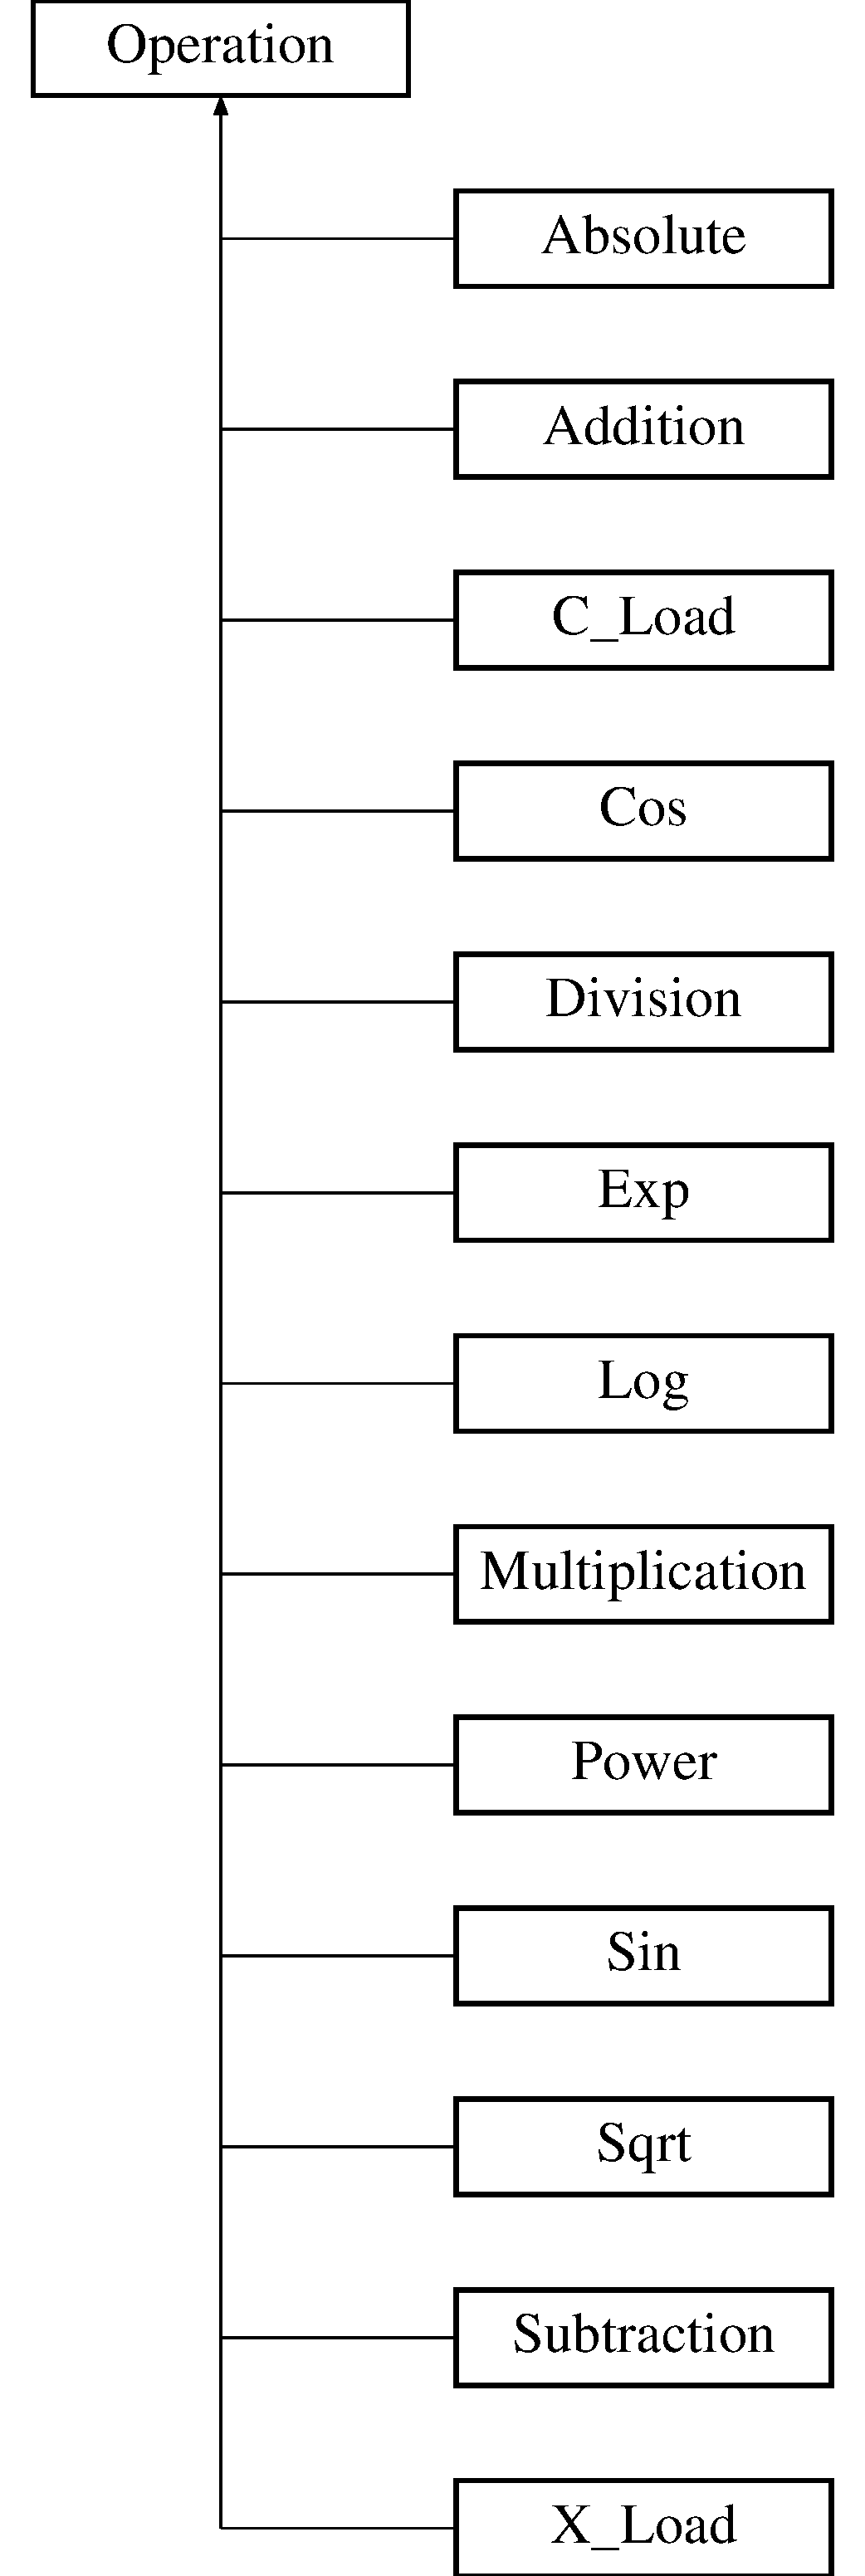
\includegraphics[height=12.000000cm]{classOperation}
\end{center}
\end{figure}
\subsection*{Public Member Functions}
\begin{DoxyCompactItemize}
\item 
virtual int \hyperlink{classOperation_ae6af21e893ca28e13471e2f7879afd3e}{get\+\_\+arity} ()=0\hypertarget{classOperation_ae6af21e893ca28e13471e2f7879afd3e}{}\label{classOperation_ae6af21e893ca28e13471e2f7879afd3e}

\begin{DoxyCompactList}\small\item\em Returns how many parameters the operation requires. \end{DoxyCompactList}\item 
virtual std\+::string \hyperlink{classOperation_aa905714b34d5cc518fa9b248682f4ee7}{get\+\_\+print} ()=0\hypertarget{classOperation_aa905714b34d5cc518fa9b248682f4ee7}{}\label{classOperation_aa905714b34d5cc518fa9b248682f4ee7}

\begin{DoxyCompactList}\small\item\em Returns the string representation of the operator. \end{DoxyCompactList}\item 
virtual void \hyperlink{classOperation_a89093eb53f975dd98b6a36d85fa17276}{evaluate} (const Eigen\+::\+Array\+X3i \&stack, const Eigen\+::\+Array\+X\+Xd \&x, const Eigen\+::\+Vector\+Xd \&constants, std\+::vector$<$ Eigen\+::\+Array\+X\+Xd $>$ \&buffer, std\+::size\+\_\+t result\+\_\+location)=0
\begin{DoxyCompactList}\small\item\em evaluates a single command at the location passed in \end{DoxyCompactList}\item 
virtual void \hyperlink{classOperation_a42b611d08c6b00568c5d1b08688ebcce}{deriv\+\_\+evaluate} (const Eigen\+::\+Array\+X3i \&stack, const int command\+\_\+index, const std\+::vector$<$ Eigen\+::\+Array\+X\+Xd $>$ \&forward\+\_\+buffer, std\+::vector$<$ Eigen\+::\+Array\+X\+Xd $>$ \&reverse\+\_\+buffer, int dependency)=0
\begin{DoxyCompactList}\small\item\em Computes reverse autodiff partial of a command stack. \end{DoxyCompactList}\end{DoxyCompactItemize}


\subsection{Detailed Description}
Abstract class for an operation. 

This is the abstract class for the \hyperlink{classOperation}{Operation} being performed.

\begin{DoxyNote}{Note}
Operators include \+: \hyperlink{classX__Load}{X\+\_\+\+Load}, \hyperlink{classC__Load}{C\+\_\+\+Load}, \hyperlink{classAddition}{Addition}, \hyperlink{classSubtraction}{Subtraction}, \hyperlink{classMultiplication}{Multiplication}, \hyperlink{classDivision}{Division}, sin, cos, exp, log, pow, abs, sqrt 
\end{DoxyNote}


\subsection{Member Function Documentation}
\index{Operation@{Operation}!deriv\+\_\+evaluate@{deriv\+\_\+evaluate}}
\index{deriv\+\_\+evaluate@{deriv\+\_\+evaluate}!Operation@{Operation}}
\subsubsection[{\texorpdfstring{deriv\+\_\+evaluate(const Eigen\+::\+Array\+X3i \&stack, const int command\+\_\+index, const std\+::vector$<$ Eigen\+::\+Array\+X\+Xd $>$ \&forward\+\_\+buffer, std\+::vector$<$ Eigen\+::\+Array\+X\+Xd $>$ \&reverse\+\_\+buffer, int dependency)=0}{deriv_evaluate(const Eigen::ArrayX3i &stack, const int command_index, const std::vector< Eigen::ArrayXXd > &forward_buffer, std::vector< Eigen::ArrayXXd > &reverse_buffer, int dependency)=0}}]{\setlength{\rightskip}{0pt plus 5cm}virtual void Operation\+::deriv\+\_\+evaluate (
\begin{DoxyParamCaption}
\item[{const Eigen\+::\+Array\+X3i \&}]{stack, }
\item[{const int}]{command\+\_\+index, }
\item[{const std\+::vector$<$ Eigen\+::\+Array\+X\+Xd $>$ \&}]{forward\+\_\+buffer, }
\item[{std\+::vector$<$ Eigen\+::\+Array\+X\+Xd $>$ \&}]{reverse\+\_\+buffer, }
\item[{int}]{dependency}
\end{DoxyParamCaption}
)\hspace{0.3cm}{\ttfamily [pure virtual]}}\hypertarget{classOperation_a42b611d08c6b00568c5d1b08688ebcce}{}\label{classOperation_a42b611d08c6b00568c5d1b08688ebcce}


Computes reverse autodiff partial of a command stack. 


\begin{DoxyParams}[1]{Parameters}
\mbox{\tt in}  & {\em stack} & The stack that contains each command. Eigen\+::\+Array\+X3i \\
\hline
\mbox{\tt in}  & {\em command\+\_\+index} & Index of command in the command; also the location of the result to be placed in the reverse buffer. \\
\hline
\mbox{\tt in}  & {\em forward\+\_\+buffer} & Vector of Eigen arrays for the forward buffer. \\
\hline
 & {\em } & \\
\hline
\end{DoxyParams}


Implemented in \hyperlink{classSqrt_aa85791e8fd1f7239b34aed9f21a9f3a6}{Sqrt}, \hyperlink{classAbsolute_a8c75e9e1efcfd1fc50ee2af13ed9d6d1}{Absolute}, \hyperlink{classPower_aacb7fa5a44485f39df757f5a8b134d28}{Power}, \hyperlink{classLog_a6f52d16f62171275092117364faa9b04}{Log}, \hyperlink{classExp_aaf9e4870dcd8eda83174f003d9bd4a8a}{Exp}, \hyperlink{classCos_a4ca2ae643db43a16772f9fdbb86c06a6}{Cos}, \hyperlink{classSin_a7ee9713a0e86b56b7cb4f23f81b1a502}{Sin}, \hyperlink{classDivision_af0f88f306718e3a490315e4be78885f3}{Division}, \hyperlink{classMultiplication_add5b53fbcd0f2e16c3be398c53d0fbe6}{Multiplication}, \hyperlink{classSubtraction_aabe4bc428dcc778adb63940a3e91327d}{Subtraction}, \hyperlink{classAddition_a30c3e7495cbe3bdc010f2d3f8570bcc8}{Addition}, \hyperlink{classC__Load_abfe90cef11f940a216284970f6db7b0d}{C\+\_\+\+Load}, and \hyperlink{classX__Load_a5ee414b0a344871b8e52d5c9c6c2f51b}{X\+\_\+\+Load}.

\index{Operation@{Operation}!evaluate@{evaluate}}
\index{evaluate@{evaluate}!Operation@{Operation}}
\subsubsection[{\texorpdfstring{evaluate(const Eigen\+::\+Array\+X3i \&stack, const Eigen\+::\+Array\+X\+Xd \&x, const Eigen\+::\+Vector\+Xd \&constants, std\+::vector$<$ Eigen\+::\+Array\+X\+Xd $>$ \&buffer, std\+::size\+\_\+t result\+\_\+location)=0}{evaluate(const Eigen::ArrayX3i &stack, const Eigen::ArrayXXd &x, const Eigen::VectorXd &constants, std::vector< Eigen::ArrayXXd > &buffer, std::size_t result_location)=0}}]{\setlength{\rightskip}{0pt plus 5cm}virtual void Operation\+::evaluate (
\begin{DoxyParamCaption}
\item[{const Eigen\+::\+Array\+X3i \&}]{stack, }
\item[{const Eigen\+::\+Array\+X\+Xd \&}]{x, }
\item[{const Eigen\+::\+Vector\+Xd \&}]{constants, }
\item[{std\+::vector$<$ Eigen\+::\+Array\+X\+Xd $>$ \&}]{buffer, }
\item[{std\+::size\+\_\+t}]{result\+\_\+location}
\end{DoxyParamCaption}
)\hspace{0.3cm}{\ttfamily [pure virtual]}}\hypertarget{classOperation_a89093eb53f975dd98b6a36d85fa17276}{}\label{classOperation_a89093eb53f975dd98b6a36d85fa17276}


evaluates a single command at the location passed in 


\begin{DoxyParams}[1]{Parameters}
\mbox{\tt in}  & {\em stack} & The stack that contains each command. Eigen\+::\+Array\+X3i \\
\hline
\mbox{\tt in}  & {\em x} & Input variables to the acyclic graph. Eigen\+::\+Array\+X\+Xd \\
\hline
\mbox{\tt in}  & {\em constants} & Constants used in the command. Eigen\+::\+Vector\+Xd \\
\hline
 & {\em } & \\
\hline
\end{DoxyParams}


Implemented in \hyperlink{classSqrt_aa0f673292c8980fe03061c5f0f85339d}{Sqrt}, \hyperlink{classAbsolute_a841ddbf6d5c0e8ad3950208946f9ad75}{Absolute}, \hyperlink{classPower_a3e672a4654976e92496e05c5c1d78ccd}{Power}, \hyperlink{classLog_af5402c400512ee9dfe17698929683bbc}{Log}, \hyperlink{classExp_a12142e937f2fa11002ebe3d574626aa5}{Exp}, \hyperlink{classCos_a580742a5758d0e31ecfc98c9e49fa597}{Cos}, \hyperlink{classSin_a1eee9fe523f2facfb47360eff481277b}{Sin}, \hyperlink{classDivision_a09bcc06557768b3a3abc31667ab03103}{Division}, \hyperlink{classMultiplication_a19044777a8cc6ba3bc662d1fbadb7b28}{Multiplication}, \hyperlink{classSubtraction_af0628604da8b47a69ab666a507b7b58d}{Subtraction}, \hyperlink{classAddition_a2fe0b74f5aaf992389f39db8e47c671f}{Addition}, \hyperlink{classC__Load_a82be394b7e177cc378def30ff9972941}{C\+\_\+\+Load}, and \hyperlink{classX__Load_ab2725c1a3843f12e4f0730aefbcaedd9}{X\+\_\+\+Load}.



The documentation for this class was generated from the following file\+:\begin{DoxyCompactItemize}
\item 
/users0/gbomarit/\+Projects/\+Genetic\+\_\+\+Programming/bingo/bingocpp/include/\+Bingo\+Cpp/acyclic\+\_\+graph\+\_\+nodes.\+h\end{DoxyCompactItemize}

\hypertarget{classOperatorInterface}{}\section{Operator\+Interface Class Reference}
\label{classOperatorInterface}\index{Operator\+Interface@{Operator\+Interface}}


Populate and hold the map of operations.  




{\ttfamily \#include $<$acyclic\+\_\+graph\+\_\+nodes.\+h$>$}

\subsection*{Static Public Member Functions}
\begin{DoxyCompactItemize}
\item 
static std\+::map$<$ int, \hyperlink{classOperation}{Operation} $\ast$ $>$ {\bfseries create\+\_\+op\+\_\+map} ()\hypertarget{classOperatorInterface_ab9027be9ca1976893ed083b05c067d13}{}\label{classOperatorInterface_ab9027be9ca1976893ed083b05c067d13}

\end{DoxyCompactItemize}
\subsection*{Static Public Attributes}
\begin{DoxyCompactItemize}
\item 
static std\+::map$<$ int, \hyperlink{classOperation}{Operation} $\ast$ $>$ {\bfseries operator\+\_\+map}
\end{DoxyCompactItemize}


\subsection{Detailed Description}
Populate and hold the map of operations. 

\subsection{Member Data Documentation}
\index{Operator\+Interface@{Operator\+Interface}!operator\+\_\+map@{operator\+\_\+map}}
\index{operator\+\_\+map@{operator\+\_\+map}!Operator\+Interface@{Operator\+Interface}}
\subsubsection[{\texorpdfstring{operator\+\_\+map}{operator_map}}]{\setlength{\rightskip}{0pt plus 5cm}std\+::map$<$ int, {\bf Operation} $\ast$ $>$ Operator\+Interface\+::operator\+\_\+map\hspace{0.3cm}{\ttfamily [static]}}\hypertarget{classOperatorInterface_a90337c660b5c440182b4d7bcd2b49e61}{}\label{classOperatorInterface_a90337c660b5c440182b4d7bcd2b49e61}
{\bfseries Initial value\+:}
\begin{DoxyCode}
=
  OperatorInterface::create\_op\_map()
\end{DoxyCode}


The documentation for this class was generated from the following files\+:\begin{DoxyCompactItemize}
\item 
/users0/gbomarit/\+Projects/\+Genetic\+\_\+\+Programming/bingo/bingocpp/include/\+Bingo\+Cpp/acyclic\+\_\+graph\+\_\+nodes.\+h\item 
/users0/gbomarit/\+Projects/\+Genetic\+\_\+\+Programming/bingo/bingocpp/src/acyclic\+\_\+graph\+\_\+nodes.\+cpp\end{DoxyCompactItemize}

\hypertarget{classPower}{}\section{Power Class Reference}
\label{classPower}\index{Power@{Power}}


This class performs power.  




{\ttfamily \#include $<$acyclic\+\_\+graph\+\_\+nodes.\+h$>$}

Inheritance diagram for Power\+:\begin{figure}[H]
\begin{center}
\leavevmode
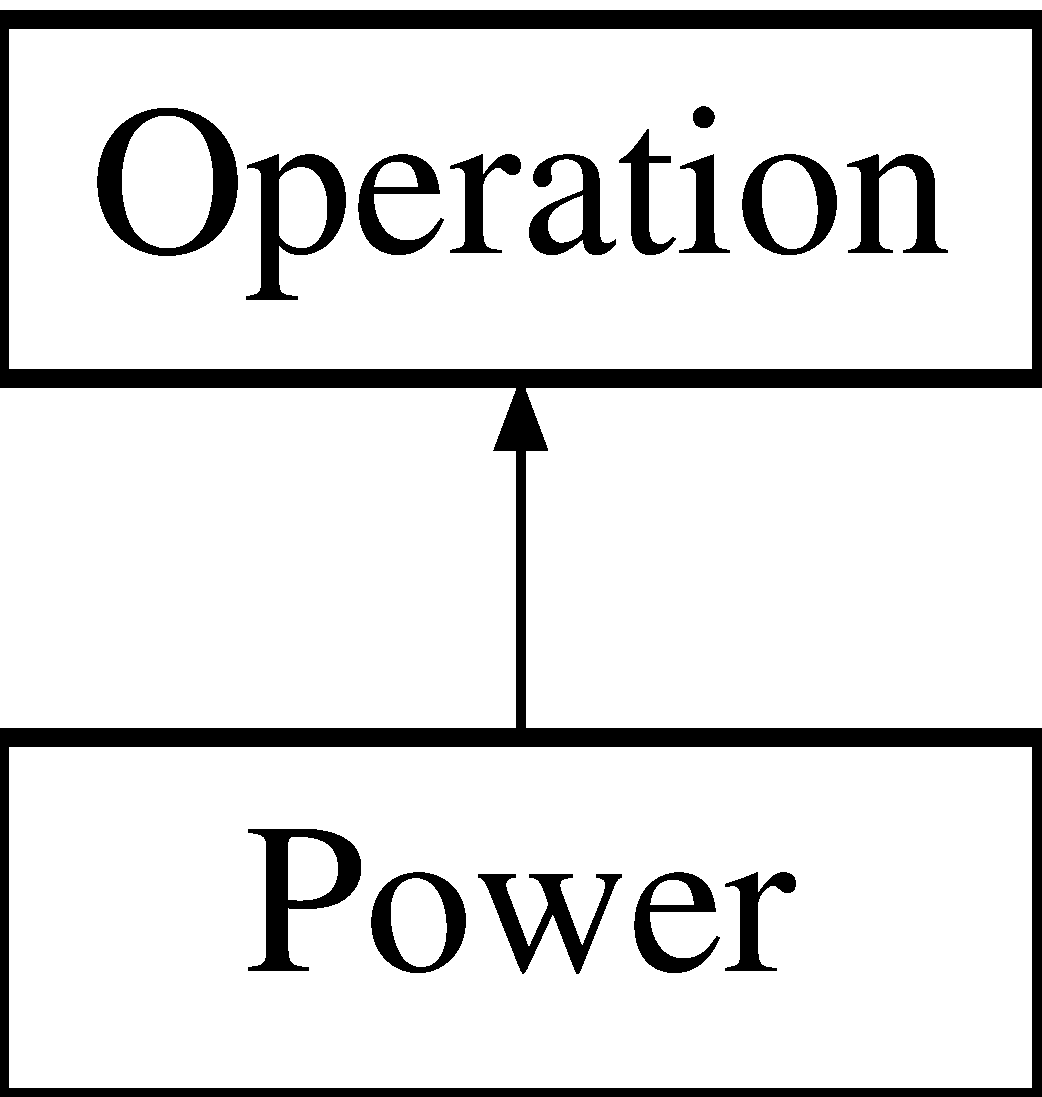
\includegraphics[height=2.000000cm]{classPower}
\end{center}
\end{figure}
\subsection*{Public Member Functions}
\begin{DoxyCompactItemize}
\item 
int \hyperlink{classPower_a07b02c15e12345a186bc2f5904df87d7}{get\+\_\+arity} ()\hypertarget{classPower_a07b02c15e12345a186bc2f5904df87d7}{}\label{classPower_a07b02c15e12345a186bc2f5904df87d7}

\begin{DoxyCompactList}\small\item\em Returns how many parameters the operation requires. \end{DoxyCompactList}\item 
std\+::string \hyperlink{classPower_a89b7b5eb5f1073ac4a20ee9eff9ea232}{get\+\_\+print} ()\hypertarget{classPower_a89b7b5eb5f1073ac4a20ee9eff9ea232}{}\label{classPower_a89b7b5eb5f1073ac4a20ee9eff9ea232}

\begin{DoxyCompactList}\small\item\em Returns the string representation of the operator. \end{DoxyCompactList}\item 
virtual void \hyperlink{classPower_a3e672a4654976e92496e05c5c1d78ccd}{evaluate} (const Eigen\+::\+Array\+X3i \&stack, const Eigen\+::\+Array\+X\+Xd \&x, const Eigen\+::\+Vector\+Xd \&constants, std\+::vector$<$ Eigen\+::\+Array\+X\+Xd $>$ \&buffer, std\+::size\+\_\+t result\+\_\+location)
\begin{DoxyCompactList}\small\item\em evaluates a single command at the location passed in \end{DoxyCompactList}\item 
virtual void \hyperlink{classPower_aacb7fa5a44485f39df757f5a8b134d28}{deriv\+\_\+evaluate} (const Eigen\+::\+Array\+X3i \&stack, const int command\+\_\+index, const std\+::vector$<$ Eigen\+::\+Array\+X\+Xd $>$ \&forward\+\_\+buffer, std\+::vector$<$ Eigen\+::\+Array\+X\+Xd $>$ \&reverse\+\_\+buffer, int dependency)
\begin{DoxyCompactList}\small\item\em Computes reverse autodiff partial of a command stack. \end{DoxyCompactList}\end{DoxyCompactItemize}


\subsection{Detailed Description}
This class performs power. 

\subsection{Member Function Documentation}
\index{Power@{Power}!deriv\+\_\+evaluate@{deriv\+\_\+evaluate}}
\index{deriv\+\_\+evaluate@{deriv\+\_\+evaluate}!Power@{Power}}
\subsubsection[{\texorpdfstring{deriv\+\_\+evaluate(const Eigen\+::\+Array\+X3i \&stack, const int command\+\_\+index, const std\+::vector$<$ Eigen\+::\+Array\+X\+Xd $>$ \&forward\+\_\+buffer, std\+::vector$<$ Eigen\+::\+Array\+X\+Xd $>$ \&reverse\+\_\+buffer, int dependency)}{deriv_evaluate(const Eigen::ArrayX3i &stack, const int command_index, const std::vector< Eigen::ArrayXXd > &forward_buffer, std::vector< Eigen::ArrayXXd > &reverse_buffer, int dependency)}}]{\setlength{\rightskip}{0pt plus 5cm}void Power\+::deriv\+\_\+evaluate (
\begin{DoxyParamCaption}
\item[{const Eigen\+::\+Array\+X3i \&}]{stack, }
\item[{const int}]{command\+\_\+index, }
\item[{const std\+::vector$<$ Eigen\+::\+Array\+X\+Xd $>$ \&}]{forward\+\_\+buffer, }
\item[{std\+::vector$<$ Eigen\+::\+Array\+X\+Xd $>$ \&}]{reverse\+\_\+buffer, }
\item[{int}]{dependency}
\end{DoxyParamCaption}
)\hspace{0.3cm}{\ttfamily [virtual]}}\hypertarget{classPower_aacb7fa5a44485f39df757f5a8b134d28}{}\label{classPower_aacb7fa5a44485f39df757f5a8b134d28}


Computes reverse autodiff partial of a command stack. 


\begin{DoxyParams}[1]{Parameters}
\mbox{\tt in}  & {\em stack} & The stack that contains each command. Eigen\+::\+Array\+X3i \\
\hline
\mbox{\tt in}  & {\em command\+\_\+index} & Index of command in the command; also the location of the result to be placed in the reverse buffer. \\
\hline
\mbox{\tt in}  & {\em forward\+\_\+buffer} & Vector of Eigen arrays for the forward buffer. \\
\hline
 & {\em } & \\
\hline
\end{DoxyParams}


Implements \hyperlink{classOperation_a42b611d08c6b00568c5d1b08688ebcce}{Operation}.

\index{Power@{Power}!evaluate@{evaluate}}
\index{evaluate@{evaluate}!Power@{Power}}
\subsubsection[{\texorpdfstring{evaluate(const Eigen\+::\+Array\+X3i \&stack, const Eigen\+::\+Array\+X\+Xd \&x, const Eigen\+::\+Vector\+Xd \&constants, std\+::vector$<$ Eigen\+::\+Array\+X\+Xd $>$ \&buffer, std\+::size\+\_\+t result\+\_\+location)}{evaluate(const Eigen::ArrayX3i &stack, const Eigen::ArrayXXd &x, const Eigen::VectorXd &constants, std::vector< Eigen::ArrayXXd > &buffer, std::size_t result_location)}}]{\setlength{\rightskip}{0pt plus 5cm}void Power\+::evaluate (
\begin{DoxyParamCaption}
\item[{const Eigen\+::\+Array\+X3i \&}]{stack, }
\item[{const Eigen\+::\+Array\+X\+Xd \&}]{x, }
\item[{const Eigen\+::\+Vector\+Xd \&}]{constants, }
\item[{std\+::vector$<$ Eigen\+::\+Array\+X\+Xd $>$ \&}]{buffer, }
\item[{std\+::size\+\_\+t}]{result\+\_\+location}
\end{DoxyParamCaption}
)\hspace{0.3cm}{\ttfamily [virtual]}}\hypertarget{classPower_a3e672a4654976e92496e05c5c1d78ccd}{}\label{classPower_a3e672a4654976e92496e05c5c1d78ccd}


evaluates a single command at the location passed in 


\begin{DoxyParams}[1]{Parameters}
\mbox{\tt in}  & {\em stack} & The stack that contains each command. Eigen\+::\+Array\+X3i \\
\hline
\mbox{\tt in}  & {\em x} & Input variables to the acyclic graph. Eigen\+::\+Array\+X\+Xd \\
\hline
\mbox{\tt in}  & {\em constants} & Constants used in the command. Eigen\+::\+Vector\+Xd \\
\hline
 & {\em } & \\
\hline
\end{DoxyParams}


Implements \hyperlink{classOperation_a89093eb53f975dd98b6a36d85fa17276}{Operation}.



The documentation for this class was generated from the following files\+:\begin{DoxyCompactItemize}
\item 
/users0/gbomarit/\+Projects/\+Genetic\+\_\+\+Programming/bingo/bingocpp/include/\+Bingo\+Cpp/acyclic\+\_\+graph\+\_\+nodes.\+h\item 
/users0/gbomarit/\+Projects/\+Genetic\+\_\+\+Programming/bingo/bingocpp/src/acyclic\+\_\+graph\+\_\+nodes.\+cpp\end{DoxyCompactItemize}

\hypertarget{classSin}{}\section{Sin Class Reference}
\label{classSin}\index{Sin@{Sin}}


This class performs sine.  




{\ttfamily \#include $<$acyclic\+\_\+graph\+\_\+nodes.\+h$>$}

Inheritance diagram for Sin\+:\begin{figure}[H]
\begin{center}
\leavevmode
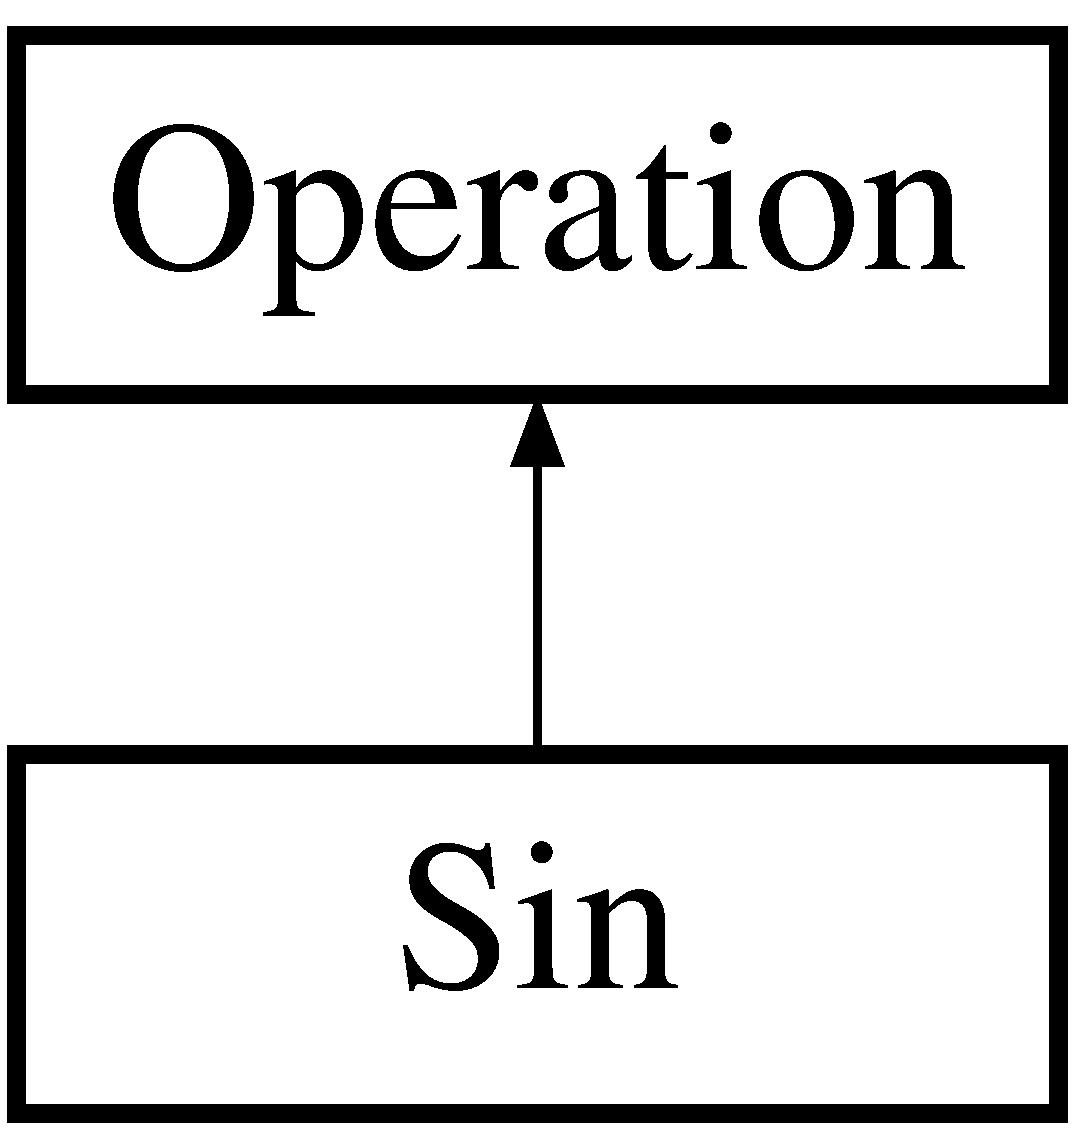
\includegraphics[height=2.000000cm]{classSin}
\end{center}
\end{figure}
\subsection*{Public Member Functions}
\begin{DoxyCompactItemize}
\item 
int \hyperlink{classSin_af9defcb92f8a2ddd5785b631f3b7296d}{get\+\_\+arity} ()\hypertarget{classSin_af9defcb92f8a2ddd5785b631f3b7296d}{}\label{classSin_af9defcb92f8a2ddd5785b631f3b7296d}

\begin{DoxyCompactList}\small\item\em Returns how many parameters the operation requires. \end{DoxyCompactList}\item 
std\+::string \hyperlink{classSin_a126a29e052db561151e42cf9d778bd8b}{get\+\_\+print} ()\hypertarget{classSin_a126a29e052db561151e42cf9d778bd8b}{}\label{classSin_a126a29e052db561151e42cf9d778bd8b}

\begin{DoxyCompactList}\small\item\em Returns the string representation of the operator. \end{DoxyCompactList}\item 
virtual void \hyperlink{classSin_a1eee9fe523f2facfb47360eff481277b}{evaluate} (const Eigen\+::\+Array\+X3i \&stack, const Eigen\+::\+Array\+X\+Xd \&x, const Eigen\+::\+Vector\+Xd \&constants, std\+::vector$<$ Eigen\+::\+Array\+X\+Xd $>$ \&buffer, std\+::size\+\_\+t result\+\_\+location)
\begin{DoxyCompactList}\small\item\em evaluates a single command at the location passed in \end{DoxyCompactList}\item 
virtual void \hyperlink{classSin_a7ee9713a0e86b56b7cb4f23f81b1a502}{deriv\+\_\+evaluate} (const Eigen\+::\+Array\+X3i \&stack, const int command\+\_\+index, const std\+::vector$<$ Eigen\+::\+Array\+X\+Xd $>$ \&forward\+\_\+buffer, std\+::vector$<$ Eigen\+::\+Array\+X\+Xd $>$ \&reverse\+\_\+buffer, int dependency)
\begin{DoxyCompactList}\small\item\em Computes reverse autodiff partial of a command stack. \end{DoxyCompactList}\end{DoxyCompactItemize}


\subsection{Detailed Description}
This class performs sine. 

\subsection{Member Function Documentation}
\index{Sin@{Sin}!deriv\+\_\+evaluate@{deriv\+\_\+evaluate}}
\index{deriv\+\_\+evaluate@{deriv\+\_\+evaluate}!Sin@{Sin}}
\subsubsection[{\texorpdfstring{deriv\+\_\+evaluate(const Eigen\+::\+Array\+X3i \&stack, const int command\+\_\+index, const std\+::vector$<$ Eigen\+::\+Array\+X\+Xd $>$ \&forward\+\_\+buffer, std\+::vector$<$ Eigen\+::\+Array\+X\+Xd $>$ \&reverse\+\_\+buffer, int dependency)}{deriv_evaluate(const Eigen::ArrayX3i &stack, const int command_index, const std::vector< Eigen::ArrayXXd > &forward_buffer, std::vector< Eigen::ArrayXXd > &reverse_buffer, int dependency)}}]{\setlength{\rightskip}{0pt plus 5cm}void Sin\+::deriv\+\_\+evaluate (
\begin{DoxyParamCaption}
\item[{const Eigen\+::\+Array\+X3i \&}]{stack, }
\item[{const int}]{command\+\_\+index, }
\item[{const std\+::vector$<$ Eigen\+::\+Array\+X\+Xd $>$ \&}]{forward\+\_\+buffer, }
\item[{std\+::vector$<$ Eigen\+::\+Array\+X\+Xd $>$ \&}]{reverse\+\_\+buffer, }
\item[{int}]{dependency}
\end{DoxyParamCaption}
)\hspace{0.3cm}{\ttfamily [virtual]}}\hypertarget{classSin_a7ee9713a0e86b56b7cb4f23f81b1a502}{}\label{classSin_a7ee9713a0e86b56b7cb4f23f81b1a502}


Computes reverse autodiff partial of a command stack. 


\begin{DoxyParams}[1]{Parameters}
\mbox{\tt in}  & {\em stack} & The stack that contains each command. Eigen\+::\+Array\+X3i \\
\hline
\mbox{\tt in}  & {\em command\+\_\+index} & Index of command in the command; also the location of the result to be placed in the reverse buffer. \\
\hline
\mbox{\tt in}  & {\em forward\+\_\+buffer} & Vector of Eigen arrays for the forward buffer. \\
\hline
 & {\em } & \\
\hline
\end{DoxyParams}


Implements \hyperlink{classOperation_a42b611d08c6b00568c5d1b08688ebcce}{Operation}.

\index{Sin@{Sin}!evaluate@{evaluate}}
\index{evaluate@{evaluate}!Sin@{Sin}}
\subsubsection[{\texorpdfstring{evaluate(const Eigen\+::\+Array\+X3i \&stack, const Eigen\+::\+Array\+X\+Xd \&x, const Eigen\+::\+Vector\+Xd \&constants, std\+::vector$<$ Eigen\+::\+Array\+X\+Xd $>$ \&buffer, std\+::size\+\_\+t result\+\_\+location)}{evaluate(const Eigen::ArrayX3i &stack, const Eigen::ArrayXXd &x, const Eigen::VectorXd &constants, std::vector< Eigen::ArrayXXd > &buffer, std::size_t result_location)}}]{\setlength{\rightskip}{0pt plus 5cm}void Sin\+::evaluate (
\begin{DoxyParamCaption}
\item[{const Eigen\+::\+Array\+X3i \&}]{stack, }
\item[{const Eigen\+::\+Array\+X\+Xd \&}]{x, }
\item[{const Eigen\+::\+Vector\+Xd \&}]{constants, }
\item[{std\+::vector$<$ Eigen\+::\+Array\+X\+Xd $>$ \&}]{buffer, }
\item[{std\+::size\+\_\+t}]{result\+\_\+location}
\end{DoxyParamCaption}
)\hspace{0.3cm}{\ttfamily [virtual]}}\hypertarget{classSin_a1eee9fe523f2facfb47360eff481277b}{}\label{classSin_a1eee9fe523f2facfb47360eff481277b}


evaluates a single command at the location passed in 


\begin{DoxyParams}[1]{Parameters}
\mbox{\tt in}  & {\em stack} & The stack that contains each command. Eigen\+::\+Array\+X3i \\
\hline
\mbox{\tt in}  & {\em x} & Input variables to the acyclic graph. Eigen\+::\+Array\+X\+Xd \\
\hline
\mbox{\tt in}  & {\em constants} & Constants used in the command. Eigen\+::\+Vector\+Xd \\
\hline
 & {\em } & \\
\hline
\end{DoxyParams}


Implements \hyperlink{classOperation_a89093eb53f975dd98b6a36d85fa17276}{Operation}.



The documentation for this class was generated from the following files\+:\begin{DoxyCompactItemize}
\item 
/users0/gbomarit/\+Projects/\+Genetic\+\_\+\+Programming/bingo/bingocpp/include/\+Bingo\+Cpp/acyclic\+\_\+graph\+\_\+nodes.\+h\item 
/users0/gbomarit/\+Projects/\+Genetic\+\_\+\+Programming/bingo/bingocpp/src/acyclic\+\_\+graph\+\_\+nodes.\+cpp\end{DoxyCompactItemize}

\hypertarget{classSqrt}{}\section{Sqrt Class Reference}
\label{classSqrt}\index{Sqrt@{Sqrt}}


This class performs square root.  




{\ttfamily \#include $<$acyclic\+\_\+graph\+\_\+nodes.\+h$>$}

Inheritance diagram for Sqrt\+:\begin{figure}[H]
\begin{center}
\leavevmode
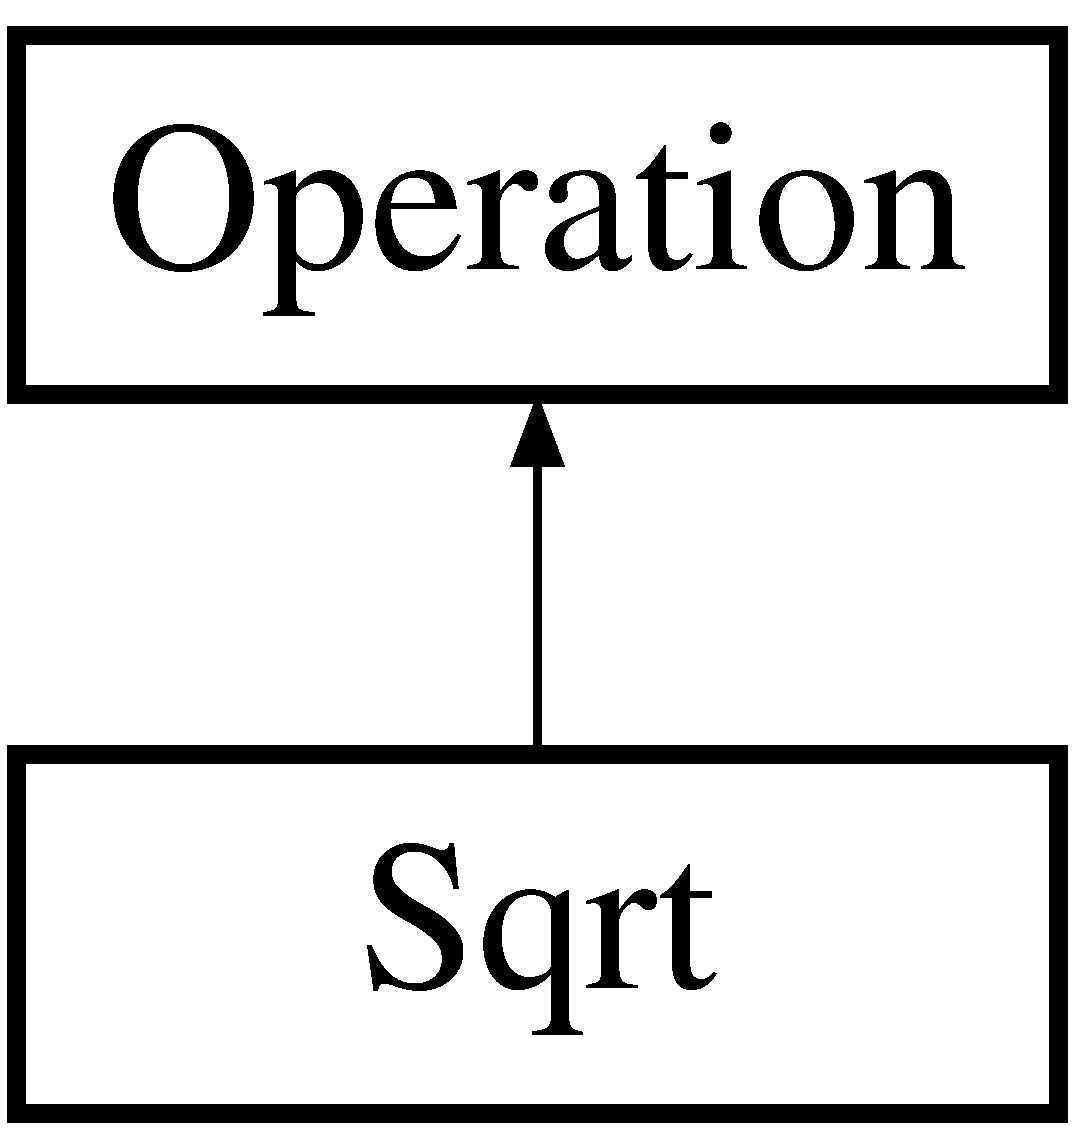
\includegraphics[height=2.000000cm]{classSqrt}
\end{center}
\end{figure}
\subsection*{Public Member Functions}
\begin{DoxyCompactItemize}
\item 
int \hyperlink{classSqrt_af9e7bd53427b5d56bf70a9958c793964}{get\+\_\+arity} ()\hypertarget{classSqrt_af9e7bd53427b5d56bf70a9958c793964}{}\label{classSqrt_af9e7bd53427b5d56bf70a9958c793964}

\begin{DoxyCompactList}\small\item\em Returns how many parameters the operation requires. \end{DoxyCompactList}\item 
std\+::string \hyperlink{classSqrt_ad219db03b8559e643e48c859e741ab1a}{get\+\_\+print} ()\hypertarget{classSqrt_ad219db03b8559e643e48c859e741ab1a}{}\label{classSqrt_ad219db03b8559e643e48c859e741ab1a}

\begin{DoxyCompactList}\small\item\em Returns the string representation of the operator. \end{DoxyCompactList}\item 
virtual void \hyperlink{classSqrt_aa0f673292c8980fe03061c5f0f85339d}{evaluate} (const Eigen\+::\+Array\+X3i \&stack, const Eigen\+::\+Array\+X\+Xd \&x, const Eigen\+::\+Vector\+Xd \&constants, std\+::vector$<$ Eigen\+::\+Array\+X\+Xd $>$ \&buffer, std\+::size\+\_\+t result\+\_\+location)
\begin{DoxyCompactList}\small\item\em evaluates a single command at the location passed in \end{DoxyCompactList}\item 
virtual void \hyperlink{classSqrt_aa85791e8fd1f7239b34aed9f21a9f3a6}{deriv\+\_\+evaluate} (const Eigen\+::\+Array\+X3i \&stack, const int command\+\_\+index, const std\+::vector$<$ Eigen\+::\+Array\+X\+Xd $>$ \&forward\+\_\+buffer, std\+::vector$<$ Eigen\+::\+Array\+X\+Xd $>$ \&reverse\+\_\+buffer, int dependency)
\begin{DoxyCompactList}\small\item\em Computes reverse autodiff partial of a command stack. \end{DoxyCompactList}\end{DoxyCompactItemize}


\subsection{Detailed Description}
This class performs square root. 

\subsection{Member Function Documentation}
\index{Sqrt@{Sqrt}!deriv\+\_\+evaluate@{deriv\+\_\+evaluate}}
\index{deriv\+\_\+evaluate@{deriv\+\_\+evaluate}!Sqrt@{Sqrt}}
\subsubsection[{\texorpdfstring{deriv\+\_\+evaluate(const Eigen\+::\+Array\+X3i \&stack, const int command\+\_\+index, const std\+::vector$<$ Eigen\+::\+Array\+X\+Xd $>$ \&forward\+\_\+buffer, std\+::vector$<$ Eigen\+::\+Array\+X\+Xd $>$ \&reverse\+\_\+buffer, int dependency)}{deriv_evaluate(const Eigen::ArrayX3i &stack, const int command_index, const std::vector< Eigen::ArrayXXd > &forward_buffer, std::vector< Eigen::ArrayXXd > &reverse_buffer, int dependency)}}]{\setlength{\rightskip}{0pt plus 5cm}void Sqrt\+::deriv\+\_\+evaluate (
\begin{DoxyParamCaption}
\item[{const Eigen\+::\+Array\+X3i \&}]{stack, }
\item[{const int}]{command\+\_\+index, }
\item[{const std\+::vector$<$ Eigen\+::\+Array\+X\+Xd $>$ \&}]{forward\+\_\+buffer, }
\item[{std\+::vector$<$ Eigen\+::\+Array\+X\+Xd $>$ \&}]{reverse\+\_\+buffer, }
\item[{int}]{dependency}
\end{DoxyParamCaption}
)\hspace{0.3cm}{\ttfamily [virtual]}}\hypertarget{classSqrt_aa85791e8fd1f7239b34aed9f21a9f3a6}{}\label{classSqrt_aa85791e8fd1f7239b34aed9f21a9f3a6}


Computes reverse autodiff partial of a command stack. 


\begin{DoxyParams}[1]{Parameters}
\mbox{\tt in}  & {\em stack} & The stack that contains each command. Eigen\+::\+Array\+X3i \\
\hline
\mbox{\tt in}  & {\em command\+\_\+index} & Index of command in the command; also the location of the result to be placed in the reverse buffer. \\
\hline
\mbox{\tt in}  & {\em forward\+\_\+buffer} & Vector of Eigen arrays for the forward buffer. \\
\hline
 & {\em } & \\
\hline
\end{DoxyParams}


Implements \hyperlink{classOperation_a42b611d08c6b00568c5d1b08688ebcce}{Operation}.

\index{Sqrt@{Sqrt}!evaluate@{evaluate}}
\index{evaluate@{evaluate}!Sqrt@{Sqrt}}
\subsubsection[{\texorpdfstring{evaluate(const Eigen\+::\+Array\+X3i \&stack, const Eigen\+::\+Array\+X\+Xd \&x, const Eigen\+::\+Vector\+Xd \&constants, std\+::vector$<$ Eigen\+::\+Array\+X\+Xd $>$ \&buffer, std\+::size\+\_\+t result\+\_\+location)}{evaluate(const Eigen::ArrayX3i &stack, const Eigen::ArrayXXd &x, const Eigen::VectorXd &constants, std::vector< Eigen::ArrayXXd > &buffer, std::size_t result_location)}}]{\setlength{\rightskip}{0pt plus 5cm}void Sqrt\+::evaluate (
\begin{DoxyParamCaption}
\item[{const Eigen\+::\+Array\+X3i \&}]{stack, }
\item[{const Eigen\+::\+Array\+X\+Xd \&}]{x, }
\item[{const Eigen\+::\+Vector\+Xd \&}]{constants, }
\item[{std\+::vector$<$ Eigen\+::\+Array\+X\+Xd $>$ \&}]{buffer, }
\item[{std\+::size\+\_\+t}]{result\+\_\+location}
\end{DoxyParamCaption}
)\hspace{0.3cm}{\ttfamily [virtual]}}\hypertarget{classSqrt_aa0f673292c8980fe03061c5f0f85339d}{}\label{classSqrt_aa0f673292c8980fe03061c5f0f85339d}


evaluates a single command at the location passed in 


\begin{DoxyParams}[1]{Parameters}
\mbox{\tt in}  & {\em stack} & The stack that contains each command. Eigen\+::\+Array\+X3i \\
\hline
\mbox{\tt in}  & {\em x} & Input variables to the acyclic graph. Eigen\+::\+Array\+X\+Xd \\
\hline
\mbox{\tt in}  & {\em constants} & Constants used in the command. Eigen\+::\+Vector\+Xd \\
\hline
 & {\em } & \\
\hline
\end{DoxyParams}


Implements \hyperlink{classOperation_a89093eb53f975dd98b6a36d85fa17276}{Operation}.



The documentation for this class was generated from the following files\+:\begin{DoxyCompactItemize}
\item 
/users0/gbomarit/\+Projects/\+Genetic\+\_\+\+Programming/bingo/bingocpp/include/\+Bingo\+Cpp/acyclic\+\_\+graph\+\_\+nodes.\+h\item 
/users0/gbomarit/\+Projects/\+Genetic\+\_\+\+Programming/bingo/bingocpp/src/acyclic\+\_\+graph\+\_\+nodes.\+cpp\end{DoxyCompactItemize}

\hypertarget{structStandardRegression}{}\section{Standard\+Regression Struct Reference}
\label{structStandardRegression}\index{Standard\+Regression@{Standard\+Regression}}


Traditional fitness evaluation.  




{\ttfamily \#include $<$fitness\+\_\+metric.\+h$>$}

Inheritance diagram for Standard\+Regression\+:\begin{figure}[H]
\begin{center}
\leavevmode
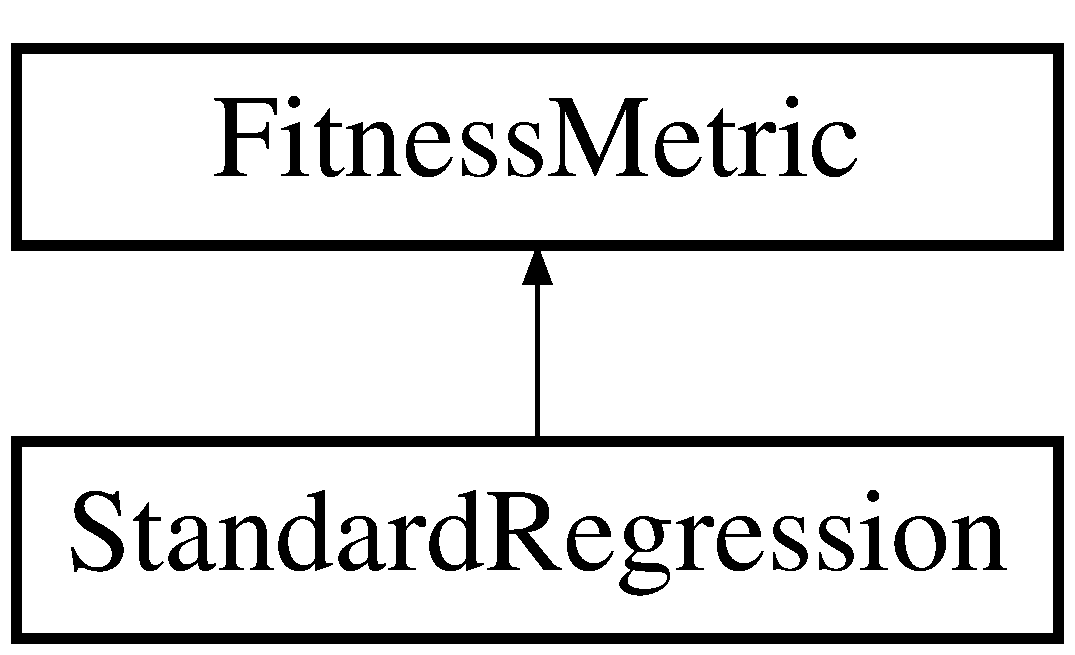
\includegraphics[height=2.000000cm]{structStandardRegression}
\end{center}
\end{figure}
\subsection*{Public Member Functions}
\begin{DoxyCompactItemize}
\item 
Eigen\+::\+Array\+X\+Xd \hyperlink{structStandardRegression_a0c35e5b8ce369988c8e1d6c3249b9581}{evaluate\+\_\+fitness\+\_\+vector} (\hyperlink{classAcyclicGraph}{Acyclic\+Graph} \&indv, \hyperlink{structTrainingData}{Training\+Data} \&train)
\begin{DoxyCompactList}\small\item\em f(x) -\/ y where f is defined by indv and x, y are in train \end{DoxyCompactList}\end{DoxyCompactItemize}


\subsection{Detailed Description}
Traditional fitness evaluation. 

\subsection{Member Function Documentation}
\index{Standard\+Regression@{Standard\+Regression}!evaluate\+\_\+fitness\+\_\+vector@{evaluate\+\_\+fitness\+\_\+vector}}
\index{evaluate\+\_\+fitness\+\_\+vector@{evaluate\+\_\+fitness\+\_\+vector}!Standard\+Regression@{Standard\+Regression}}
\subsubsection[{\texorpdfstring{evaluate\+\_\+fitness\+\_\+vector(\+Acyclic\+Graph \&indv, Training\+Data \&train)}{evaluate_fitness_vector(AcyclicGraph &indv, TrainingData &train)}}]{\setlength{\rightskip}{0pt plus 5cm}Eigen\+::\+Array\+X\+Xd Standard\+Regression\+::evaluate\+\_\+fitness\+\_\+vector (
\begin{DoxyParamCaption}
\item[{{\bf Acyclic\+Graph} \&}]{indv, }
\item[{{\bf Training\+Data} \&}]{train}
\end{DoxyParamCaption}
)\hspace{0.3cm}{\ttfamily [virtual]}}\hypertarget{structStandardRegression_a0c35e5b8ce369988c8e1d6c3249b9581}{}\label{structStandardRegression_a0c35e5b8ce369988c8e1d6c3249b9581}


f(x) -\/ y where f is defined by indv and x, y are in train 

\begin{DoxyNote}{Note}
Each implementation will need to hard code casting \hyperlink{structTrainingData}{Training\+Data} to a specific type in this function.
\end{DoxyNote}

\begin{DoxyParams}[1]{Parameters}
\mbox{\tt in}  & {\em indv} & agcpp indv to be evaluated. \hyperlink{classAcyclicGraph}{Acyclic\+Graph} \\
\hline
\mbox{\tt in}  & {\em train} & The \hyperlink{structTrainingData}{Training\+Data} to evaluate the fitness. \hyperlink{structTrainingData}{Training\+Data} \\
\hline
\end{DoxyParams}
\begin{DoxyReturn}{Returns}
Eigen\+::\+Array\+X\+Xd the fitness vector 
\end{DoxyReturn}


Implements \hyperlink{structFitnessMetric_a17bf921d3200dc93493e2af5c38552ad}{Fitness\+Metric}.



The documentation for this struct was generated from the following files\+:\begin{DoxyCompactItemize}
\item 
/users0/gbomarit/\+Projects/\+Genetic\+\_\+\+Programming/bingo/bingocpp/include/\+Bingo\+Cpp/\hyperlink{fitness__metric_8h}{fitness\+\_\+metric.\+h}\item 
/users0/gbomarit/\+Projects/\+Genetic\+\_\+\+Programming/bingo/bingocpp/src/fitness\+\_\+metric.\+cpp\end{DoxyCompactItemize}

\hypertarget{classSubtraction}{}\section{Subtraction Class Reference}
\label{classSubtraction}\index{Subtraction@{Subtraction}}


This class performs subtraction.  




{\ttfamily \#include $<$acyclic\+\_\+graph\+\_\+nodes.\+h$>$}

Inheritance diagram for Subtraction\+:\begin{figure}[H]
\begin{center}
\leavevmode
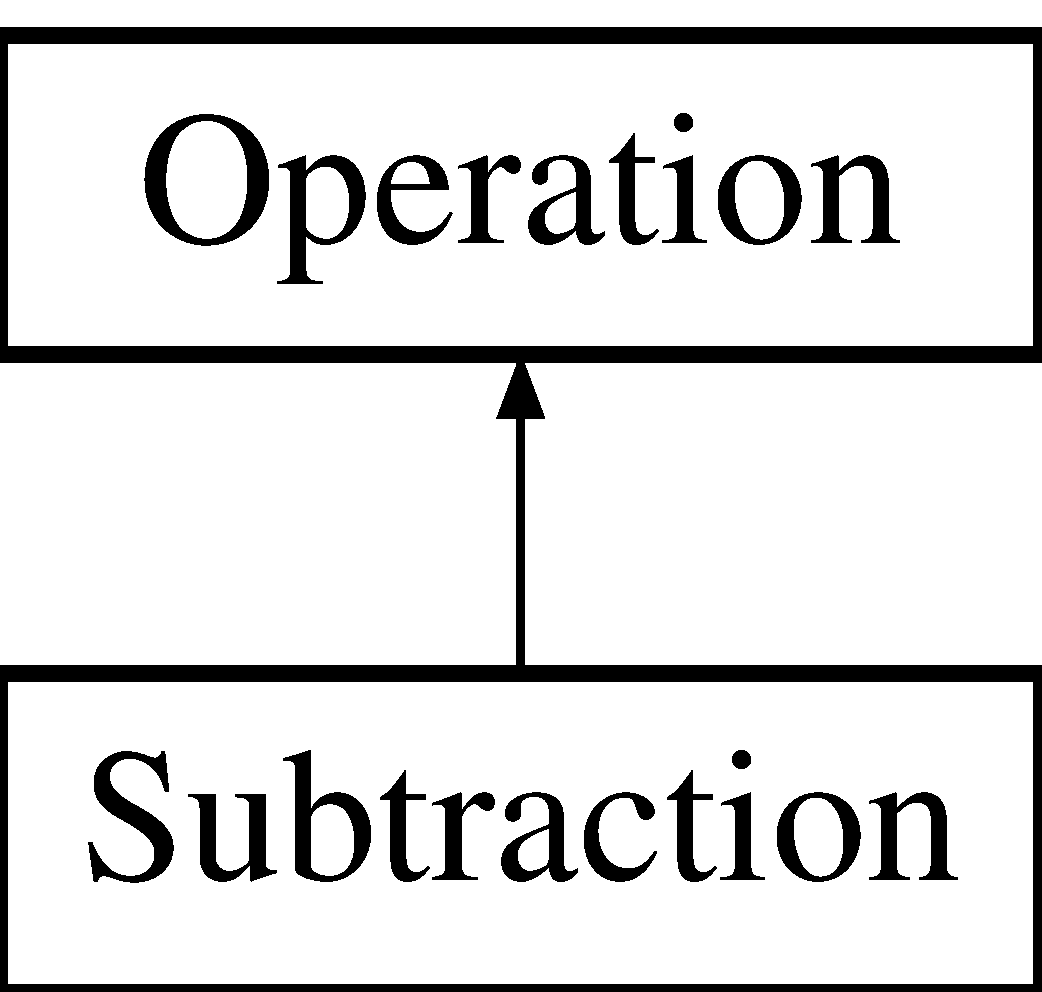
\includegraphics[height=2.000000cm]{classSubtraction}
\end{center}
\end{figure}
\subsection*{Public Member Functions}
\begin{DoxyCompactItemize}
\item 
int \hyperlink{classSubtraction_a0ecd0c6d95631fea8c73d166a30831e8}{get\+\_\+arity} ()\hypertarget{classSubtraction_a0ecd0c6d95631fea8c73d166a30831e8}{}\label{classSubtraction_a0ecd0c6d95631fea8c73d166a30831e8}

\begin{DoxyCompactList}\small\item\em Returns how many parameters the operation requires. \end{DoxyCompactList}\item 
std\+::string \hyperlink{classSubtraction_a9de7e0f8e324423dcfb7691d41545e21}{get\+\_\+print} ()\hypertarget{classSubtraction_a9de7e0f8e324423dcfb7691d41545e21}{}\label{classSubtraction_a9de7e0f8e324423dcfb7691d41545e21}

\begin{DoxyCompactList}\small\item\em Returns the string representation of the operator. \end{DoxyCompactList}\item 
virtual void \hyperlink{classSubtraction_af0628604da8b47a69ab666a507b7b58d}{evaluate} (const Eigen\+::\+Array\+X3i \&stack, const Eigen\+::\+Array\+X\+Xd \&x, const Eigen\+::\+Vector\+Xd \&constants, std\+::vector$<$ Eigen\+::\+Array\+X\+Xd $>$ \&buffer, std\+::size\+\_\+t result\+\_\+location)
\begin{DoxyCompactList}\small\item\em evaluates a single command at the location passed in \end{DoxyCompactList}\item 
virtual void \hyperlink{classSubtraction_aabe4bc428dcc778adb63940a3e91327d}{deriv\+\_\+evaluate} (const Eigen\+::\+Array\+X3i \&stack, const int command\+\_\+index, const std\+::vector$<$ Eigen\+::\+Array\+X\+Xd $>$ \&forward\+\_\+buffer, std\+::vector$<$ Eigen\+::\+Array\+X\+Xd $>$ \&reverse\+\_\+buffer, int dependency)
\begin{DoxyCompactList}\small\item\em Computes reverse autodiff partial of a command stack. \end{DoxyCompactList}\end{DoxyCompactItemize}


\subsection{Detailed Description}
This class performs subtraction. 

\subsection{Member Function Documentation}
\index{Subtraction@{Subtraction}!deriv\+\_\+evaluate@{deriv\+\_\+evaluate}}
\index{deriv\+\_\+evaluate@{deriv\+\_\+evaluate}!Subtraction@{Subtraction}}
\subsubsection[{\texorpdfstring{deriv\+\_\+evaluate(const Eigen\+::\+Array\+X3i \&stack, const int command\+\_\+index, const std\+::vector$<$ Eigen\+::\+Array\+X\+Xd $>$ \&forward\+\_\+buffer, std\+::vector$<$ Eigen\+::\+Array\+X\+Xd $>$ \&reverse\+\_\+buffer, int dependency)}{deriv_evaluate(const Eigen::ArrayX3i &stack, const int command_index, const std::vector< Eigen::ArrayXXd > &forward_buffer, std::vector< Eigen::ArrayXXd > &reverse_buffer, int dependency)}}]{\setlength{\rightskip}{0pt plus 5cm}void Subtraction\+::deriv\+\_\+evaluate (
\begin{DoxyParamCaption}
\item[{const Eigen\+::\+Array\+X3i \&}]{stack, }
\item[{const int}]{command\+\_\+index, }
\item[{const std\+::vector$<$ Eigen\+::\+Array\+X\+Xd $>$ \&}]{forward\+\_\+buffer, }
\item[{std\+::vector$<$ Eigen\+::\+Array\+X\+Xd $>$ \&}]{reverse\+\_\+buffer, }
\item[{int}]{dependency}
\end{DoxyParamCaption}
)\hspace{0.3cm}{\ttfamily [virtual]}}\hypertarget{classSubtraction_aabe4bc428dcc778adb63940a3e91327d}{}\label{classSubtraction_aabe4bc428dcc778adb63940a3e91327d}


Computes reverse autodiff partial of a command stack. 


\begin{DoxyParams}[1]{Parameters}
\mbox{\tt in}  & {\em stack} & The stack that contains each command. Eigen\+::\+Array\+X3i \\
\hline
\mbox{\tt in}  & {\em command\+\_\+index} & Index of command in the command; also the location of the result to be placed in the reverse buffer. \\
\hline
\mbox{\tt in}  & {\em forward\+\_\+buffer} & Vector of Eigen arrays for the forward buffer. \\
\hline
 & {\em } & \\
\hline
\end{DoxyParams}


Implements \hyperlink{classOperation_a42b611d08c6b00568c5d1b08688ebcce}{Operation}.

\index{Subtraction@{Subtraction}!evaluate@{evaluate}}
\index{evaluate@{evaluate}!Subtraction@{Subtraction}}
\subsubsection[{\texorpdfstring{evaluate(const Eigen\+::\+Array\+X3i \&stack, const Eigen\+::\+Array\+X\+Xd \&x, const Eigen\+::\+Vector\+Xd \&constants, std\+::vector$<$ Eigen\+::\+Array\+X\+Xd $>$ \&buffer, std\+::size\+\_\+t result\+\_\+location)}{evaluate(const Eigen::ArrayX3i &stack, const Eigen::ArrayXXd &x, const Eigen::VectorXd &constants, std::vector< Eigen::ArrayXXd > &buffer, std::size_t result_location)}}]{\setlength{\rightskip}{0pt plus 5cm}void Subtraction\+::evaluate (
\begin{DoxyParamCaption}
\item[{const Eigen\+::\+Array\+X3i \&}]{stack, }
\item[{const Eigen\+::\+Array\+X\+Xd \&}]{x, }
\item[{const Eigen\+::\+Vector\+Xd \&}]{constants, }
\item[{std\+::vector$<$ Eigen\+::\+Array\+X\+Xd $>$ \&}]{buffer, }
\item[{std\+::size\+\_\+t}]{result\+\_\+location}
\end{DoxyParamCaption}
)\hspace{0.3cm}{\ttfamily [virtual]}}\hypertarget{classSubtraction_af0628604da8b47a69ab666a507b7b58d}{}\label{classSubtraction_af0628604da8b47a69ab666a507b7b58d}


evaluates a single command at the location passed in 


\begin{DoxyParams}[1]{Parameters}
\mbox{\tt in}  & {\em stack} & The stack that contains each command. Eigen\+::\+Array\+X3i \\
\hline
\mbox{\tt in}  & {\em x} & Input variables to the acyclic graph. Eigen\+::\+Array\+X\+Xd \\
\hline
\mbox{\tt in}  & {\em constants} & Constants used in the command. Eigen\+::\+Vector\+Xd \\
\hline
 & {\em } & \\
\hline
\end{DoxyParams}


Implements \hyperlink{classOperation_a89093eb53f975dd98b6a36d85fa17276}{Operation}.



The documentation for this class was generated from the following files\+:\begin{DoxyCompactItemize}
\item 
/users0/gbomarit/\+Projects/\+Genetic\+\_\+\+Programming/bingo/bingocpp/include/\+Bingo\+Cpp/acyclic\+\_\+graph\+\_\+nodes.\+h\item 
/users0/gbomarit/\+Projects/\+Genetic\+\_\+\+Programming/bingo/bingocpp/src/acyclic\+\_\+graph\+\_\+nodes.\+cpp\end{DoxyCompactItemize}

\hypertarget{structTrainingData}{}\section{Training\+Data Struct Reference}
\label{structTrainingData}\index{Training\+Data@{Training\+Data}}


{\ttfamily \#include $<$training\+\_\+data.\+h$>$}

Inheritance diagram for Training\+Data\+:\begin{figure}[H]
\begin{center}
\leavevmode
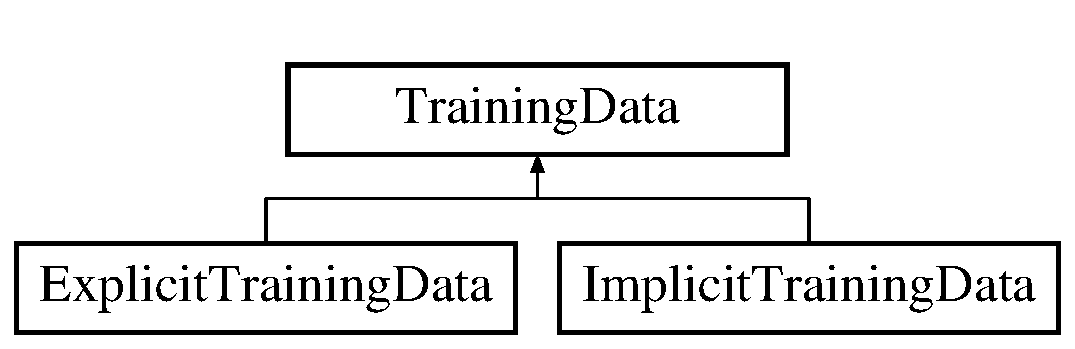
\includegraphics[height=2.000000cm]{structTrainingData}
\end{center}
\end{figure}
\subsection*{Public Member Functions}
\begin{DoxyCompactItemize}
\item 
virtual \hyperlink{structTrainingData}{Training\+Data} $\ast$ \hyperlink{structTrainingData_a96ef790e9e78909f84ce83692c7faced}{get\+\_\+item} (std\+::list$<$ int $>$ items)=0
\begin{DoxyCompactList}\small\item\em gets a new training data with certain rows \end{DoxyCompactList}\item 
virtual int \hyperlink{structTrainingData_a9be21e878961cc347e6820eb34db0a1b}{size} ()=0
\begin{DoxyCompactList}\small\item\em gets the size of x \end{DoxyCompactList}\end{DoxyCompactItemize}


\subsection{Detailed Description}
An abstract struct to hold the data for fitness calculations

\begin{DoxyNote}{Note}
\hyperlink{structTrainingData}{Training\+Data} includes \+: Implicit and Explicit data 
\end{DoxyNote}


\subsection{Member Function Documentation}
\index{Training\+Data@{Training\+Data}!get\+\_\+item@{get\+\_\+item}}
\index{get\+\_\+item@{get\+\_\+item}!Training\+Data@{Training\+Data}}
\subsubsection[{\texorpdfstring{get\+\_\+item(std\+::list$<$ int $>$ items)=0}{get_item(std::list< int > items)=0}}]{\setlength{\rightskip}{0pt plus 5cm}virtual {\bf Training\+Data}$\ast$ Training\+Data\+::get\+\_\+item (
\begin{DoxyParamCaption}
\item[{std\+::list$<$ int $>$}]{items}
\end{DoxyParamCaption}
)\hspace{0.3cm}{\ttfamily [pure virtual]}}\hypertarget{structTrainingData_a96ef790e9e78909f84ce83692c7faced}{}\label{structTrainingData_a96ef790e9e78909f84ce83692c7faced}


gets a new training data with certain rows 


\begin{DoxyParams}[1]{Parameters}
\mbox{\tt in}  & {\em items} & The rows to retrieve. std\+::list$<$int$>$ \\
\hline
\end{DoxyParams}
\begin{DoxyReturn}{Returns}
Training\+Data$\ast$ with the selected data 
\end{DoxyReturn}


Implemented in \hyperlink{structImplicitTrainingData_a91e92604cc19a693ac89eb7dbd9fab80}{Implicit\+Training\+Data}, and \hyperlink{structExplicitTrainingData_a7c60c1b5ea185580a5842c5cca18c7d0}{Explicit\+Training\+Data}.

\index{Training\+Data@{Training\+Data}!size@{size}}
\index{size@{size}!Training\+Data@{Training\+Data}}
\subsubsection[{\texorpdfstring{size()=0}{size()=0}}]{\setlength{\rightskip}{0pt plus 5cm}virtual int Training\+Data\+::size (
\begin{DoxyParamCaption}
{}
\end{DoxyParamCaption}
)\hspace{0.3cm}{\ttfamily [pure virtual]}}\hypertarget{structTrainingData_a9be21e878961cc347e6820eb34db0a1b}{}\label{structTrainingData_a9be21e878961cc347e6820eb34db0a1b}


gets the size of x 

\begin{DoxyReturn}{Returns}
int the amount of rows in x 
\end{DoxyReturn}


Implemented in \hyperlink{structImplicitTrainingData_aa3be8b04a160fb496668bba52507d3e4}{Implicit\+Training\+Data}, and \hyperlink{structExplicitTrainingData_aa5a3da99babf2436bdb9b4652a217584}{Explicit\+Training\+Data}.



The documentation for this struct was generated from the following file\+:\begin{DoxyCompactItemize}
\item 
/users0/gbomarit/\+Projects/\+Genetic\+\_\+\+Programming/bingo/bingocpp/include/\+Bingo\+Cpp/\hyperlink{training__data_8h}{training\+\_\+data.\+h}\end{DoxyCompactItemize}

\hypertarget{classX__Load}{}\section{X\+\_\+\+Load Class Reference}
\label{classX__Load}\index{X\+\_\+\+Load@{X\+\_\+\+Load}}


This class loads the X.  




{\ttfamily \#include $<$acyclic\+\_\+graph\+\_\+nodes.\+h$>$}

Inheritance diagram for X\+\_\+\+Load\+:\begin{figure}[H]
\begin{center}
\leavevmode
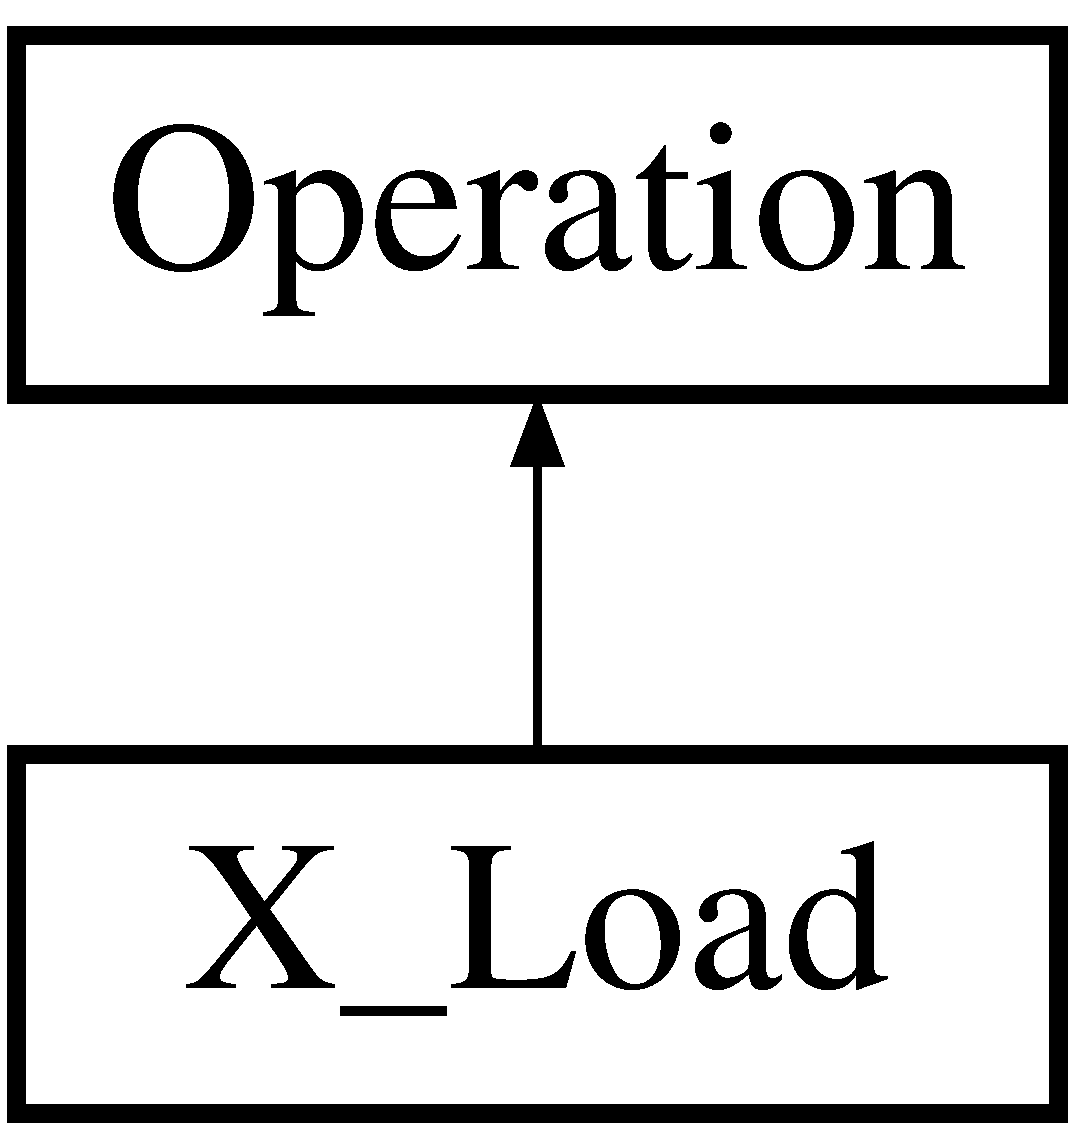
\includegraphics[height=2.000000cm]{classX__Load}
\end{center}
\end{figure}
\subsection*{Public Member Functions}
\begin{DoxyCompactItemize}
\item 
int \hyperlink{classX__Load_a04ac1ceb5aba1a29dcc77234136de802}{get\+\_\+arity} ()\hypertarget{classX__Load_a04ac1ceb5aba1a29dcc77234136de802}{}\label{classX__Load_a04ac1ceb5aba1a29dcc77234136de802}

\begin{DoxyCompactList}\small\item\em Returns how many parameters the operation requires. \end{DoxyCompactList}\item 
std\+::string \hyperlink{classX__Load_af38090c6c8ebcde7f221f6dd15f80bdb}{get\+\_\+print} ()\hypertarget{classX__Load_af38090c6c8ebcde7f221f6dd15f80bdb}{}\label{classX__Load_af38090c6c8ebcde7f221f6dd15f80bdb}

\begin{DoxyCompactList}\small\item\em Returns the string representation of the operator. \end{DoxyCompactList}\item 
virtual void \hyperlink{classX__Load_ab2725c1a3843f12e4f0730aefbcaedd9}{evaluate} (const Eigen\+::\+Array\+X3i \&stack, const Eigen\+::\+Array\+X\+Xd \&x, const Eigen\+::\+Vector\+Xd \&constants, std\+::vector$<$ Eigen\+::\+Array\+X\+Xd $>$ \&buffer, std\+::size\+\_\+t result\+\_\+location)
\begin{DoxyCompactList}\small\item\em evaluates a single command at the location passed in \end{DoxyCompactList}\item 
virtual void \hyperlink{classX__Load_a5ee414b0a344871b8e52d5c9c6c2f51b}{deriv\+\_\+evaluate} (const Eigen\+::\+Array\+X3i \&stack, const int command\+\_\+index, const std\+::vector$<$ Eigen\+::\+Array\+X\+Xd $>$ \&forward\+\_\+buffer, std\+::vector$<$ Eigen\+::\+Array\+X\+Xd $>$ \&reverse\+\_\+buffer, int dependency)
\begin{DoxyCompactList}\small\item\em Computes reverse autodiff partial of a command stack. \end{DoxyCompactList}\end{DoxyCompactItemize}


\subsection{Detailed Description}
This class loads the X. 

\subsection{Member Function Documentation}
\index{X\+\_\+\+Load@{X\+\_\+\+Load}!deriv\+\_\+evaluate@{deriv\+\_\+evaluate}}
\index{deriv\+\_\+evaluate@{deriv\+\_\+evaluate}!X\+\_\+\+Load@{X\+\_\+\+Load}}
\subsubsection[{\texorpdfstring{deriv\+\_\+evaluate(const Eigen\+::\+Array\+X3i \&stack, const int command\+\_\+index, const std\+::vector$<$ Eigen\+::\+Array\+X\+Xd $>$ \&forward\+\_\+buffer, std\+::vector$<$ Eigen\+::\+Array\+X\+Xd $>$ \&reverse\+\_\+buffer, int dependency)}{deriv_evaluate(const Eigen::ArrayX3i &stack, const int command_index, const std::vector< Eigen::ArrayXXd > &forward_buffer, std::vector< Eigen::ArrayXXd > &reverse_buffer, int dependency)}}]{\setlength{\rightskip}{0pt plus 5cm}void X\+\_\+\+Load\+::deriv\+\_\+evaluate (
\begin{DoxyParamCaption}
\item[{const Eigen\+::\+Array\+X3i \&}]{stack, }
\item[{const int}]{command\+\_\+index, }
\item[{const std\+::vector$<$ Eigen\+::\+Array\+X\+Xd $>$ \&}]{forward\+\_\+buffer, }
\item[{std\+::vector$<$ Eigen\+::\+Array\+X\+Xd $>$ \&}]{reverse\+\_\+buffer, }
\item[{int}]{dependency}
\end{DoxyParamCaption}
)\hspace{0.3cm}{\ttfamily [virtual]}}\hypertarget{classX__Load_a5ee414b0a344871b8e52d5c9c6c2f51b}{}\label{classX__Load_a5ee414b0a344871b8e52d5c9c6c2f51b}


Computes reverse autodiff partial of a command stack. 


\begin{DoxyParams}[1]{Parameters}
\mbox{\tt in}  & {\em stack} & The stack that contains each command. Eigen\+::\+Array\+X3i \\
\hline
\mbox{\tt in}  & {\em command\+\_\+index} & Index of command in the command; also the location of the result to be placed in the reverse buffer. \\
\hline
\mbox{\tt in}  & {\em forward\+\_\+buffer} & Vector of Eigen arrays for the forward buffer. \\
\hline
 & {\em } & \\
\hline
\end{DoxyParams}


Implements \hyperlink{classOperation_a42b611d08c6b00568c5d1b08688ebcce}{Operation}.

\index{X\+\_\+\+Load@{X\+\_\+\+Load}!evaluate@{evaluate}}
\index{evaluate@{evaluate}!X\+\_\+\+Load@{X\+\_\+\+Load}}
\subsubsection[{\texorpdfstring{evaluate(const Eigen\+::\+Array\+X3i \&stack, const Eigen\+::\+Array\+X\+Xd \&x, const Eigen\+::\+Vector\+Xd \&constants, std\+::vector$<$ Eigen\+::\+Array\+X\+Xd $>$ \&buffer, std\+::size\+\_\+t result\+\_\+location)}{evaluate(const Eigen::ArrayX3i &stack, const Eigen::ArrayXXd &x, const Eigen::VectorXd &constants, std::vector< Eigen::ArrayXXd > &buffer, std::size_t result_location)}}]{\setlength{\rightskip}{0pt plus 5cm}void X\+\_\+\+Load\+::evaluate (
\begin{DoxyParamCaption}
\item[{const Eigen\+::\+Array\+X3i \&}]{stack, }
\item[{const Eigen\+::\+Array\+X\+Xd \&}]{x, }
\item[{const Eigen\+::\+Vector\+Xd \&}]{constants, }
\item[{std\+::vector$<$ Eigen\+::\+Array\+X\+Xd $>$ \&}]{buffer, }
\item[{std\+::size\+\_\+t}]{result\+\_\+location}
\end{DoxyParamCaption}
)\hspace{0.3cm}{\ttfamily [virtual]}}\hypertarget{classX__Load_ab2725c1a3843f12e4f0730aefbcaedd9}{}\label{classX__Load_ab2725c1a3843f12e4f0730aefbcaedd9}


evaluates a single command at the location passed in 


\begin{DoxyParams}[1]{Parameters}
\mbox{\tt in}  & {\em stack} & The stack that contains each command. Eigen\+::\+Array\+X3i \\
\hline
\mbox{\tt in}  & {\em x} & Input variables to the acyclic graph. Eigen\+::\+Array\+X\+Xd \\
\hline
\mbox{\tt in}  & {\em constants} & Constants used in the command. Eigen\+::\+Vector\+Xd \\
\hline
 & {\em } & \\
\hline
\end{DoxyParams}


Implements \hyperlink{classOperation_a89093eb53f975dd98b6a36d85fa17276}{Operation}.



The documentation for this class was generated from the following files\+:\begin{DoxyCompactItemize}
\item 
/users0/gbomarit/\+Projects/\+Genetic\+\_\+\+Programming/bingo/bingocpp/include/\+Bingo\+Cpp/acyclic\+\_\+graph\+\_\+nodes.\+h\item 
/users0/gbomarit/\+Projects/\+Genetic\+\_\+\+Programming/bingo/bingocpp/src/acyclic\+\_\+graph\+\_\+nodes.\+cpp\end{DoxyCompactItemize}

\chapter{File Documentation}
\hypertarget{fitness__metric_8h}{}\section{/users0/gbomarit/\+Projects/\+Genetic\+\_\+\+Programming/bingo/bingocpp/include/\+Bingo\+Cpp/fitness\+\_\+metric.h File Reference}
\label{fitness__metric_8h}\index{/users0/gbomarit/\+Projects/\+Genetic\+\_\+\+Programming/bingo/bingocpp/include/\+Bingo\+Cpp/fitness\+\_\+metric.\+h@{/users0/gbomarit/\+Projects/\+Genetic\+\_\+\+Programming/bingo/bingocpp/include/\+Bingo\+Cpp/fitness\+\_\+metric.\+h}}
{\ttfamily \#include \char`\"{}Bingo\+Cpp/graph\+\_\+manip.\+h\char`\"{}}\\*
{\ttfamily \#include \char`\"{}Bingo\+Cpp/training\+\_\+data.\+h\char`\"{}}\\*
{\ttfamily \#include $<$Eigen/\+Dense$>$}\\*
{\ttfamily \#include $<$Eigen/\+Core$>$}\\*
\subsection*{Classes}
\begin{DoxyCompactItemize}
\item 
struct \hyperlink{structLMFunctor}{L\+M\+Functor}
\item 
struct \hyperlink{structFitnessMetric}{Fitness\+Metric}
\item 
struct \hyperlink{structStandardRegression}{Standard\+Regression}
\begin{DoxyCompactList}\small\item\em Traditional fitness evaluation. \end{DoxyCompactList}\item 
struct \hyperlink{structImplicitRegression}{Implicit\+Regression}
\begin{DoxyCompactList}\small\item\em Implicit Regression. \end{DoxyCompactList}\end{DoxyCompactItemize}


\subsection{Detailed Description}
\begin{DoxyAuthor}{Author}
Ethan Adams 
\end{DoxyAuthor}
\begin{DoxyDate}{Date}

\end{DoxyDate}
This file contains the cpp version of Fitness\+Metric.\+py 
\hypertarget{graph__manip_8h}{}\section{/users0/gbomarit/\+Projects/\+Genetic\+\_\+\+Programming/bingo/bingocpp/include/\+Bingo\+Cpp/graph\+\_\+manip.h File Reference}
\label{graph__manip_8h}\index{/users0/gbomarit/\+Projects/\+Genetic\+\_\+\+Programming/bingo/bingocpp/include/\+Bingo\+Cpp/graph\+\_\+manip.\+h@{/users0/gbomarit/\+Projects/\+Genetic\+\_\+\+Programming/bingo/bingocpp/include/\+Bingo\+Cpp/graph\+\_\+manip.\+h}}
{\ttfamily \#include $<$Eigen/\+Dense$>$}\\*
{\ttfamily \#include $<$Eigen/\+Core$>$}\\*
{\ttfamily \#include $<$set$>$}\\*
{\ttfamily \#include $<$map$>$}\\*
{\ttfamily \#include $<$utility$>$}\\*
{\ttfamily \#include $<$vector$>$}\\*
{\ttfamily \#include $<$string$>$}\\*
{\ttfamily \#include $<$sstream$>$}\\*
{\ttfamily \#include $<$stdlib.\+h$>$}\\*
{\ttfamily \#include $<$iomanip$>$}\\*
{\ttfamily \#include $<$time.\+h$>$}\\*
{\ttfamily \#include \char`\"{}Bingo\+Cpp/acyclic\+\_\+graph\+\_\+nodes.\+h\char`\"{}}\\*
\subsection*{Classes}
\begin{DoxyCompactItemize}
\item 
class \hyperlink{classAcyclicGraph}{Acyclic\+Graph}
\item 
class \hyperlink{classAcyclicGraphManipulator}{Acyclic\+Graph\+Manipulator}
\end{DoxyCompactItemize}


\subsection{Detailed Description}
\begin{DoxyAuthor}{Author}
Ethan Adams 
\end{DoxyAuthor}
\begin{DoxyDate}{Date}
2/26/2018
\end{DoxyDate}
This file contains the cpp version of A\+Graph\+Cpp.\+py 
\hypertarget{training__data_8h}{}\section{/users0/gbomarit/\+Projects/\+Genetic\+\_\+\+Programming/bingo/bingocpp/include/\+Bingo\+Cpp/training\+\_\+data.h File Reference}
\label{training__data_8h}\index{/users0/gbomarit/\+Projects/\+Genetic\+\_\+\+Programming/bingo/bingocpp/include/\+Bingo\+Cpp/training\+\_\+data.\+h@{/users0/gbomarit/\+Projects/\+Genetic\+\_\+\+Programming/bingo/bingocpp/include/\+Bingo\+Cpp/training\+\_\+data.\+h}}
{\ttfamily \#include $<$Eigen/\+Dense$>$}\\*
{\ttfamily \#include $<$Eigen/\+Core$>$}\\*
{\ttfamily \#include $<$vector$>$}\\*
{\ttfamily \#include $<$list$>$}\\*
\subsection*{Classes}
\begin{DoxyCompactItemize}
\item 
struct \hyperlink{structTrainingData}{Training\+Data}
\item 
struct \hyperlink{structExplicitTrainingData}{Explicit\+Training\+Data}
\begin{DoxyCompactList}\small\item\em This struct holds data for Explicit regression. \end{DoxyCompactList}\item 
struct \hyperlink{structImplicitTrainingData}{Implicit\+Training\+Data}
\begin{DoxyCompactList}\small\item\em This struct holds data for Implicit regression. \end{DoxyCompactList}\end{DoxyCompactItemize}


\subsection{Detailed Description}
\begin{DoxyAuthor}{Author}
Ethan Adams 
\end{DoxyAuthor}
\begin{DoxyDate}{Date}

\end{DoxyDate}
This file contains the cpp version of training\+\_\+data.\+py 
\hypertarget{utils_8h}{}\section{/users0/gbomarit/\+Projects/\+Genetic\+\_\+\+Programming/bingo/bingocpp/include/\+Bingo\+Cpp/utils.h File Reference}
\label{utils_8h}\index{/users0/gbomarit/\+Projects/\+Genetic\+\_\+\+Programming/bingo/bingocpp/include/\+Bingo\+Cpp/utils.\+h@{/users0/gbomarit/\+Projects/\+Genetic\+\_\+\+Programming/bingo/bingocpp/include/\+Bingo\+Cpp/utils.\+h}}
{\ttfamily \#include $<$iostream$>$}\\*
{\ttfamily \#include $<$stdlib.\+h$>$}\\*
{\ttfamily \#include $<$Eigen/\+Dense$>$}\\*
{\ttfamily \#include $<$Eigen/\+Core$>$}\\*
\subsection*{Functions}
\begin{DoxyCompactItemize}
\item 
std\+::vector$<$ Eigen\+::\+Array\+X\+Xd $>$ \hyperlink{utils_8h_a5836ec6058e585f69258a177ae67a000}{calculate\+\_\+partials} (Eigen\+::\+Array\+X\+Xd x)
\begin{DoxyCompactList}\small\item\em Calculate derivatves with respect to time (first dimension) \end{DoxyCompactList}\item 
double \hyperlink{utils_8h_a8883803c41dd3a1f8d4ff8d654d92979}{Gen\+Fact} (double a, double b)
\begin{DoxyCompactList}\small\item\em Generalized factorial. \end{DoxyCompactList}\item 
double \hyperlink{utils_8h_ac78013378e297fd448de0283399913c5}{Gram\+Poly} (double gp\+\_\+i, double gp\+\_\+m, double gp\+\_\+k, double gp\+\_\+s)
\begin{DoxyCompactList}\small\item\em Calculates the Gram Polynomial (gp\+\_\+s=0) or its gp\+\_\+s\textquotesingle{}th derivative evaluated at gp\+\_\+i, order gp\+\_\+k, over 2gp\+\_\+m+1 points. \end{DoxyCompactList}\item 
double \hyperlink{utils_8h_ad6be665a715d2863859c7571484e7cbd}{Gram\+Weight} (double gw\+\_\+i, double gw\+\_\+t, double gw\+\_\+m, double gw\+\_\+n, double gw\+\_\+s)
\begin{DoxyCompactList}\small\item\em Calculates the weight of the gw\+\_\+i\textquotesingle{}th data point for the gw\+\_\+t\textquotesingle{}th Least-\/\+Square point of the gw\+\_\+s\textquotesingle{}th derivative over 2gw\+\_\+m+1 points, order gw\+\_\+n. \end{DoxyCompactList}\item 
Eigen\+::\+Array\+X\+Xd \hyperlink{utils_8h_a477f6a4d628d505fd6b0551cf2832850}{savitzky\+\_\+golay} (Eigen\+::\+Array\+X\+Xd y, int window\+\_\+size, int order, int deriv=0)
\begin{DoxyCompactList}\small\item\em Smooth (and optionally differentiate) data with a Savitzky-\/\+Golay filter The Savitzky-\/\+Golay filter removes high frequency noise from data. It has the advantage of preserving the original shape and features of the signal better than other types of filtering approaches, such as moving averages techniques. \end{DoxyCompactList}\end{DoxyCompactItemize}


\subsection{Detailed Description}
\begin{DoxyAuthor}{Author}
Ethan Adams 
\end{DoxyAuthor}
\begin{DoxyDate}{Date}

\end{DoxyDate}
This file contains utility functions for doing and testing sybolic regression problems in the bingo package 

\subsection{Function Documentation}
\index{utils.\+h@{utils.\+h}!calculate\+\_\+partials@{calculate\+\_\+partials}}
\index{calculate\+\_\+partials@{calculate\+\_\+partials}!utils.\+h@{utils.\+h}}
\subsubsection[{\texorpdfstring{calculate\+\_\+partials(\+Eigen\+::\+Array\+X\+Xd x)}{calculate_partials(Eigen::ArrayXXd x)}}]{\setlength{\rightskip}{0pt plus 5cm}std\+::vector$<$Eigen\+::\+Array\+X\+Xd$>$ calculate\+\_\+partials (
\begin{DoxyParamCaption}
\item[{Eigen\+::\+Array\+X\+Xd}]{x}
\end{DoxyParamCaption}
)}\hypertarget{utils_8h_a5836ec6058e585f69258a177ae67a000}{}\label{utils_8h_a5836ec6058e585f69258a177ae67a000}


Calculate derivatves with respect to time (first dimension) 


\begin{DoxyParams}[1]{Parameters}
\mbox{\tt in}  & {\em x} & array in which derivatives will be calculated in the first dimension. Distinct trajectories can be specified by separating the datasets within x by rows of nan Eigen\+::\+Array\+X\+Xd \\
\hline
\end{DoxyParams}
\begin{DoxyReturn}{Returns}
std\+::vector$<$\+Eigen\+::\+Array\+X\+Xd$>$ with x array and corresponding time derivatives 
\end{DoxyReturn}
\index{utils.\+h@{utils.\+h}!Gen\+Fact@{Gen\+Fact}}
\index{Gen\+Fact@{Gen\+Fact}!utils.\+h@{utils.\+h}}
\subsubsection[{\texorpdfstring{Gen\+Fact(double a, double b)}{GenFact(double a, double b)}}]{\setlength{\rightskip}{0pt plus 5cm}double Gen\+Fact (
\begin{DoxyParamCaption}
\item[{double}]{a, }
\item[{double}]{b}
\end{DoxyParamCaption}
)}\hypertarget{utils_8h_a8883803c41dd3a1f8d4ff8d654d92979}{}\label{utils_8h_a8883803c41dd3a1f8d4ff8d654d92979}


Generalized factorial. 


\begin{DoxyParams}[1]{Parameters}
\mbox{\tt in}  & {\em a} & double \\
\hline
\mbox{\tt in}  & {\em b} & double \\
\hline
\end{DoxyParams}
\begin{DoxyReturn}{Returns}
double factorial 
\end{DoxyReturn}
\index{utils.\+h@{utils.\+h}!Gram\+Poly@{Gram\+Poly}}
\index{Gram\+Poly@{Gram\+Poly}!utils.\+h@{utils.\+h}}
\subsubsection[{\texorpdfstring{Gram\+Poly(double gp\+\_\+i, double gp\+\_\+m, double gp\+\_\+k, double gp\+\_\+s)}{GramPoly(double gp_i, double gp_m, double gp_k, double gp_s)}}]{\setlength{\rightskip}{0pt plus 5cm}double Gram\+Poly (
\begin{DoxyParamCaption}
\item[{double}]{gp\+\_\+i, }
\item[{double}]{gp\+\_\+m, }
\item[{double}]{gp\+\_\+k, }
\item[{double}]{gp\+\_\+s}
\end{DoxyParamCaption}
)}\hypertarget{utils_8h_ac78013378e297fd448de0283399913c5}{}\label{utils_8h_ac78013378e297fd448de0283399913c5}


Calculates the Gram Polynomial (gp\+\_\+s=0) or its gp\+\_\+s\textquotesingle{}th derivative evaluated at gp\+\_\+i, order gp\+\_\+k, over 2gp\+\_\+m+1 points. 


\begin{DoxyParams}[1]{Parameters}
\mbox{\tt in}  & {\em gp\+\_\+i} & double \\
\hline
\mbox{\tt in}  & {\em gp\+\_\+m} & double \\
\hline
\mbox{\tt in}  & {\em gp\+\_\+k} & double \\
\hline
\mbox{\tt in}  & {\em gp\+\_\+s} & double \\
\hline
\end{DoxyParams}
\begin{DoxyReturn}{Returns}
double polynomial 
\end{DoxyReturn}
\index{utils.\+h@{utils.\+h}!Gram\+Weight@{Gram\+Weight}}
\index{Gram\+Weight@{Gram\+Weight}!utils.\+h@{utils.\+h}}
\subsubsection[{\texorpdfstring{Gram\+Weight(double gw\+\_\+i, double gw\+\_\+t, double gw\+\_\+m, double gw\+\_\+n, double gw\+\_\+s)}{GramWeight(double gw_i, double gw_t, double gw_m, double gw_n, double gw_s)}}]{\setlength{\rightskip}{0pt plus 5cm}double Gram\+Weight (
\begin{DoxyParamCaption}
\item[{double}]{gw\+\_\+i, }
\item[{double}]{gw\+\_\+t, }
\item[{double}]{gw\+\_\+m, }
\item[{double}]{gw\+\_\+n, }
\item[{double}]{gw\+\_\+s}
\end{DoxyParamCaption}
)}\hypertarget{utils_8h_ad6be665a715d2863859c7571484e7cbd}{}\label{utils_8h_ad6be665a715d2863859c7571484e7cbd}


Calculates the weight of the gw\+\_\+i\textquotesingle{}th data point for the gw\+\_\+t\textquotesingle{}th Least-\/\+Square point of the gw\+\_\+s\textquotesingle{}th derivative over 2gw\+\_\+m+1 points, order gw\+\_\+n. 


\begin{DoxyParams}[1]{Parameters}
\mbox{\tt in}  & {\em gw\+\_\+i} & double \\
\hline
\mbox{\tt in}  & {\em gw\+\_\+t} & double \\
\hline
\mbox{\tt in}  & {\em gw\+\_\+m} & double \\
\hline
\mbox{\tt in}  & {\em gw\+\_\+n} & double \\
\hline
\mbox{\tt in}  & {\em gw\+\_\+s} & double \\
\hline
\end{DoxyParams}
\begin{DoxyReturn}{Returns}
double weight 
\end{DoxyReturn}
\index{utils.\+h@{utils.\+h}!savitzky\+\_\+golay@{savitzky\+\_\+golay}}
\index{savitzky\+\_\+golay@{savitzky\+\_\+golay}!utils.\+h@{utils.\+h}}
\subsubsection[{\texorpdfstring{savitzky\+\_\+golay(\+Eigen\+::\+Array\+X\+Xd y, int window\+\_\+size, int order, int deriv=0)}{savitzky_golay(Eigen::ArrayXXd y, int window_size, int order, int deriv=0)}}]{\setlength{\rightskip}{0pt plus 5cm}Eigen\+::\+Array\+X\+Xd savitzky\+\_\+golay (
\begin{DoxyParamCaption}
\item[{Eigen\+::\+Array\+X\+Xd}]{y, }
\item[{int}]{window\+\_\+size, }
\item[{int}]{order, }
\item[{int}]{deriv = {\ttfamily 0}}
\end{DoxyParamCaption}
)}\hypertarget{utils_8h_a477f6a4d628d505fd6b0551cf2832850}{}\label{utils_8h_a477f6a4d628d505fd6b0551cf2832850}


Smooth (and optionally differentiate) data with a Savitzky-\/\+Golay filter The Savitzky-\/\+Golay filter removes high frequency noise from data. It has the advantage of preserving the original shape and features of the signal better than other types of filtering approaches, such as moving averages techniques. 

The Savitzky-\/\+Golay is a type of low-\/pass filter, particularly suited for smoothing noisy data. The main idea behind this approach is to make for each point a least-\/square fit with a polynomial of high order over a odd-\/sized window centered at the point.

.. \mbox{[}1\mbox{]} A. Savitzky, M. J. E. Golay, Smoothing and Differentiation of Data by Simplified Least Squares Procedures. Analytical Chemistry, 1964, 36 (8), pp 1627-\/1639. .. \mbox{[}2\mbox{]} Numerical Recipes 3rd Edition\+: The Art of Scientific Computing W.\+H. Press, S.\+A. Teukolsky, W.\+T. Vetterling, B.\+P. Flannery Cambridge University Press I\+S\+B\+N-\/13\+: 9780521880688


\begin{DoxyParams}[1]{Parameters}
\mbox{\tt in}  & {\em y} & array\+\_\+like, shape (N,) the values of the time history of the signal. Eigen\+::\+Array\+X\+Xd \\
\hline
\mbox{\tt in}  & {\em window\+\_\+size} & the length of the window. Must be an odd integer number. int \\
\hline
\mbox{\tt in}  & {\em order} & the order of the polynomial used in the filtering. Must be less than window\+\_\+size -\/ 1. int \\
\hline
\mbox{\tt in}  & {\em deriv} & the order of the derivative to compute (default = 0 means only smoothing). int \\
\hline
\end{DoxyParams}
\begin{DoxyReturn}{Returns}
Eiggen\+::\+Array\+X\+Xd the smoothed signal (or it\textquotesingle{}s n-\/th derivative). 
\end{DoxyReturn}

%--- End generated contents ---

% Index
\backmatter
\newpage
\phantomsection
\clearemptydoublepage
\addcontentsline{toc}{chapter}{Index}
\printindex

\end{document}
